%%
%% Dibbler - a portable DHCPv6
%%
%% authors: Tomasz Mrugalski <thomson@klub.com.pl>
%%          Marek Senderski <msend@o2.pl>
%%
%% released under GNU GPL v2 only licence
%%
%% $Id: dibbler-user.tex,v 1.20 2008-08-29 00:07:38 thomson Exp $
%%

\documentclass[11pt]{article}
\usepackage[latin2]{inputenc}
\usepackage[dvips]{graphicx}
\usepackage{float}
\usepackage{makeidx}
\usepackage{fancyhdr}
\usepackage{indentfirst}
\usepackage{tabularx}
\usepackage{longtable}
\usepackage{url}
\usepackage[usenames]{color}
\usepackage[colorlinks=true,citecolor=darkblue,linkcolor=darkblue,urlcolor=darkred]{hyperref}

%\setlength{\topmargin}{-1.0cm}
\usepackage[twoside=true,
	    left={2cm},
	    right={2cm},
	    top={2cm},
	    bottom={2cm},
	    footskip={1cm},
	    headheight={1cm},
%%            twosideshift={0.5cm},
	    headsep={0.5cm}]{geometry}

%%%%%% \dzis macro by Lupan %%%%%%
\newcommand{\dzis}{
\the\year-%
\ifnum\month<10{}0\fi
\the\month-%
\ifnum\day<10{}0\fi
\the\day
}

\author{Tomasz Mrugalski\\ \small{\href{mailto:thomson(at)klub.com.pl}{thomson(at)klub.com.pl}}}
\date{\dzis}
\title{Dibbler -- a portable DHCPv6\\User's guide}

\definecolor{myBgColor}{rgb}{1.0,1.0,1.0}
\definecolor{darkred}{rgb}{0.7,0.2, 0.4} %% URL (external links)
\definecolor{darkblue}{rgb}{0.0,0.0,0.7} %% internal links, toc
\definecolor{myBgTableColor}{rgb}{0.9, 0.9, 0.9}
\pagecolor{myBgColor}

%% include auto-generated version number
\newcommand{\version}{1.0.0}


\pagestyle{fancy}
\fancyhf{}
\fancyhead[L]{\small\bfseries Dibbler \version}
\fancyhead[C]{\small\bfseries User's Guide}
\fancyhead[R]{\small\bfseries\thepage}
%%\fancyhead[C]{\small\bfseries\leftmark}
\renewcommand{\headrulewidth}{0.5pt}
\renewcommand{\footrulewidth}{0pt}
\addtolength{\headheight}{0.5pt}
\fancypagestyle{plain}{%
\fancyhead{} %
\renewcommand{\headrulewidth}{0pt} %
}

%%\newenvironment{Cfg}{ \Verbatim }{ \endVerbatim }

\makeindex

\newcommand{\Q}{ \vspace{0.5cm} \textbf{Q:} }
\newcommand{\A}{ \vspace{0.25cm} \textbf{A:} }
\newcommand{\Note}{ \textbf{Note:} }

\newcommand{\msg}[1]{\emph{#1}}
\newcommand{\opt}[1]{\emph{#1}}
\newcommand{\IA}{ \textbf{\emph{IA}} }
\newcommand{\duid} { DUID }
\newcommand{\code}[1]{\textbf{#1}}
\newcommand{\subsubsubsection}[1]{\subsubsection{#1}}
\newcommand{\CfgBegin}{\begin{lstlisting}}
\newcommand{\CfgEnd}{\end{lstlisting}}

%% this does not work... yet
\newenvironment{Cfg}{\begin{lstlisting}}{\end{lstlisting}}

%% for Verbatim environment
%%\RecustomVerbatimEnvironment{Verbatim}{Verbatim}{frame=single,framesep=3mm}

%%\renewcommand{\FancyVerbFormatLine}[1]{\colorbox{red}{#1}}
\usepackage{listings}
\lstset{basicstyle=\ttfamily, columns=flexible, backgroundcolor=\color{myBgTableColor},frame=lines}
%or columns=fullflexible

%% message names should be printed this way: \msg{SOLICIT}
%% options should be printed this way:       \opt{Option Request}

\begin{document}

\vspace{-4cm}
\maketitle
\vspace{-1cm}

\begin{center}
\version
\end{center}

\newpage
\tableofcontents

\newpage

%% INTRO, OVERVIEW
%%
%% Dibbler - a portable DHCPv6
%%
%% authors: Tomasz Mrugalski <thomson@klub.com.pl>
%%
%% released under GNU GPL v2 licence
%%
%%

\section{Intro}
First of all, as an author I would like to thank you for your interest
in this DHCPv6 implementation. If this documentation doesn't answer
your questions or you have any suggestions, feel free to contact
me as explained in \hyperlink{contact}{Contact} section. Also be sure
to check out Dibbler website: \url{http://klub.com.pl/dhcpv6/}.

\begin{flushright}
\emph{Tomasz Mrugalski}
\end{flushright}

\subsection{Overview}

\emph{Dynamic Host Configuration Protocol for IPv6}, often abbreviated
as DHCPv6, is a protocol, which is used to automatically configure IPv6
capable computers and other equipment located in a local network. This
protocol defines \emph{clients} (i.e. nodes, which want to be configured),
\emph{servers} (i.e. nodes, which provide configuration to clients) and
\emph{relays} (i.e. nodes, which are connected to more than one network and
are able to forward traffic between local clients and remote
servers). Also, special type of DHCPv6 entity called \emph{requestor}
has been defined. It is used by network administrator to query servers
about their status and assigned parameters.

Dibbler is a portable DHCPv6 solution, which features server, client and
relay. Currently there are ports available for many Windows platforms
ranging from NT4 to Windows 8, Linux 2.4 or later systems and Mac OS
(experimental). See Section \ref{requirements} for details. It supports both stateful
(i.e. IPv6 address granting) and stateless (i.e. options granting)
autoconfiguration. Besides basic
functionality (specified in basic DHCPv6 spec, RFC3315 \cite{rfc3315}),
it also offers serveral enhancements, e.g. DNS servers and domain names
configuration.

Dibbler is an open source software, distributed under
\href{http://www.gnu.org/copyleft/gpl.html}{GNU GPL} v2 licence. It means
that it is freely available, free of charge and can be used by anyone
(including commercial users). Source code is also provided, so anyone
skilled enough can fix bugs, add new features and distribute his/her
own version.

\emph{Requestor} support has been added in version 0.7.0RC1. Requestor
is a separate entity, which sends queries to the server regarding
leases to specific clients. It is possible to ask a server, who has
specific address or what addresses are assigned to a specific client.
This feature is part of the lease query mechanism defined in
\cite{rfc5007} and is considered advanced topic. If you don't know
what lease query is, you definetely don't need it.

\begin{figure}[ht]
\begin{center}
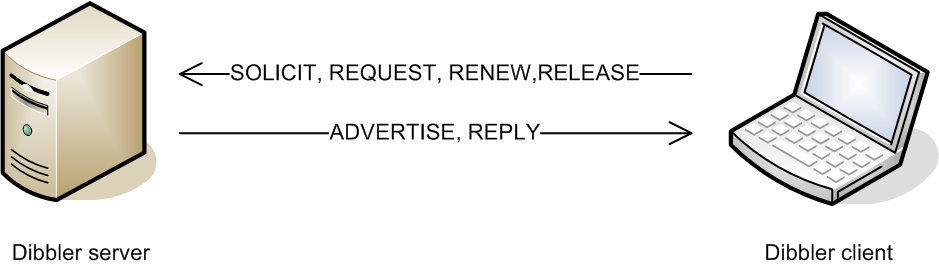
\includegraphics[width=0.7\textwidth]{dibbler-srv-cli}
\caption{\emph{General DHCPv6 operation}}
\end{center}
\end{figure}

Dibbler 1.0.0RC1 supports all features specified in RFC3315. In
particular the following features are supported:
\begin{itemize}
\item Basic server discovery and address assignment (\msg{SOLICIT},
      \msg{ADVERTISE}, \msg{REQUEST} and \msg{REPLY} messages) -- This
      is a most common case: client discovers servers available in the
      local network, then asks for an address (and possibly additional
      options like DNS configuration), which is granted by a~server.

\begin{figure}[ht]
\begin{center}
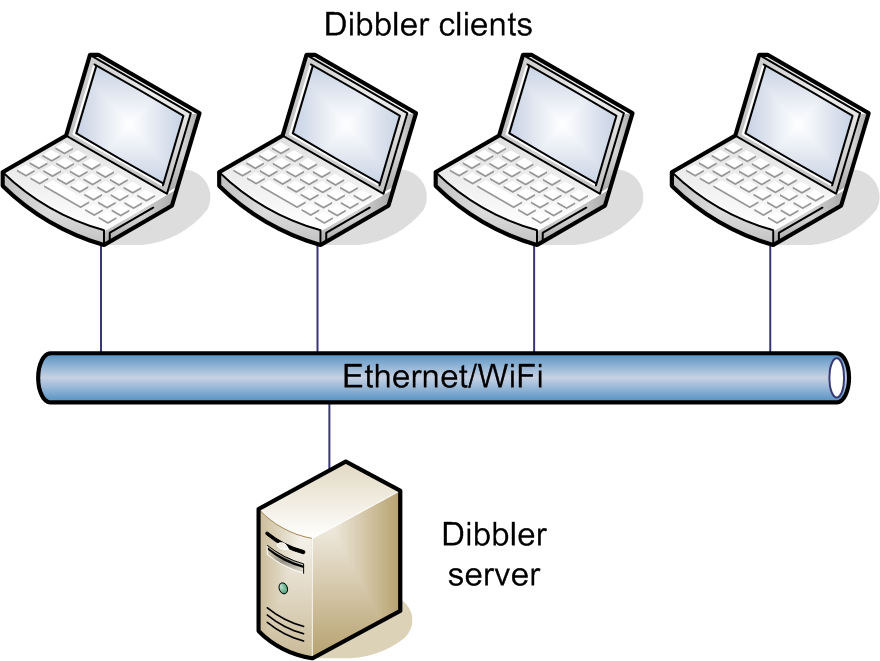
\includegraphics[width=0.6\textwidth]{dibbler-multiple-cli}
\caption{\emph{Several clients supported by one server}}
\end{center}
\end{figure}

\item Server redundancy/Best server discovery -- when client detects
      more than one server available (by receiving more than one
      \msg{ADVERTISE} message), it chooses the best one and remembers
      remaining ones as a backup.

\begin{figure}[ht]
\begin{center}
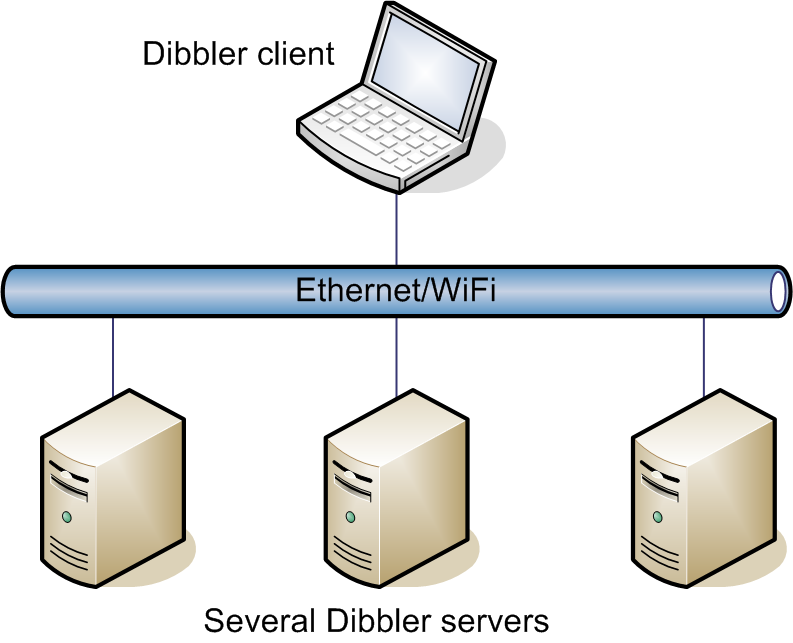
\includegraphics[width=0.6\textwidth]{dibbler-multiple-srv}
\caption{\emph{Redundancy: several servers}}
\end{center}
\end{figure}

\item Multiple servers support -- Client is capable of discovering and
  maintaning communication with several servers. For example, client
  would like to have 5 addresses configured. Prefered server can only
  lease 3, so client send request for remaining 2 addresses to one of
  the remaining servers.
\item Relay support -- In a larger network, which contains several
  Ethernet segments and/or wireless areas, sometimes centrally located
  DHCPv6 server might not be directly reachable. In such cace,
  additional proxies, so called relays, might be deployed to relay
  communication between clients and a remote server. Dibbler server
  supports indirect communication with clients via
  relays. Stand-alone, lightweight relay implementation is also
  available. Clients are capable of talking to the server directly or
  via relays.
\item Address renewal -- After receiving address from a server, client
  might be instructed to renew its address at regular
  intervals. Client periodically sends \msg{RENEW} messege to a
  server, which granted its address. In case of communication failure,
  client is also able to attempt emergency address renewal (i.e. it
  sends \msg{REBIND} message to any server).
\item Unicast communication -- if specific conditions are met, client
  could send messages directly to a server's unicast address, so
  additional servers does not need to process those messages. It also
  improves effciency, as all nodes present in LAN segment receive
  multicast packets.\footnote{Nodes, which do not belong to specific
    multicast group, drop those packets silently. However, determining
    if host belongs or not to a group must be performed on each
    node. Also using multicast communication increases the network
    load.}
\item Duplicate address detection -- Client is able to detect and
  properly handle faulty situation, when server grants an address
  which is illegaly used by some other host. It will inform server of
  such circumstances (using \msg{DECLINE} message), and request
  another address. Server will mark this address as used by unknown
  host, and will assign another address to a client.
\item Power failure/crash support -- After client recovers from a
  crash or a power failure, it still can have valid addresses
  assigned. In such circumstances, client uses \msg{CONFIRM} message,
  to config if those addresses are still valid.
\item Link change detection -- Client can be instructed to monitor its
      link state. Once it detects
\item Normal and temporary addresses -- Depending on its purpose,
      client can be configured to ask for normal (\opt{IA\_NA} option)
      or temporary (\opt{IA\_TA} option). Although use of temporary
      addresses is rather uncommon, both dibbler server and client
      support it.
\item Hint system -- Client can be configured to send various parameters
      and addresses in the \msg{REQUEST} message. It will be treated as
      a hint by the server. If such hint is valid, it will be granted
      for this client.
\item Server caching -- Server can cache granted addresses, so the same
      client will receive the same address each time it asks. Size of
      this cache can be configured.
\item Stateless mode -- Client can be configured to not ask for any
      addresses, but the configuration options only. In such case, when
      no addresses are granted, such configuration is called stateless
      (\msg{INFORMATION-REQUEST} message is used instead of normal
      \msg{REQUEST}).
\item Rapid Commit -- Sometimes it is desirable to quicken configuration
      process. If both client and server are configured to use rapid
      commit, address assignment procedure can be shortened to 2
      messages, instead of usual 4. Major advantage is lesser network
      usage and quicker client startup time.
\item M,O bits from Router Advertisement -- the client can be told to
  observe M(managed) and O(OtherConf) bits from RA and act according
  to them
\item Reconfigure -- server can inform clients that the configuration
  has changed and clients can initiate Reconfigure
\item Authentication: Reconfigure-key -- the server can generate HMAC-MD5
  reconfigure keys on the fly to later authenticate reconfigure
  messages. Clients are able to receive, store and later validate
  against that received key.
\item Authentication: Delayed authorization -- server and client can
  protect their communication against tampering by using
  preprovisioned keys.
\end{itemize}

\subsection{Supported parameters}
Except RFC3315-specified behavior \cite{rfc3315}, Dibbler also supports
several enhancements:

\begin{itemize}
\item DNS Servers -- During normal operation, almost all hosts require
      constant use of the DNS servers. It is necessary for event basic
      operations, like web surfing. DHCPv6 client can ask for
      information about DNS servers and DHCPv6 server will provide
      necessary information. \cite{rfc3646}
\item Domain Name -- Client might be interested in obtaining information
      about its domain. Properly configured domain allow reference to a
      different hosts in the same domain using hostname only, not the
      full domain name, e.g. alice.example.com with properly configured
      domain can refer to another host in the same domain by using 'bob'
      only, instead of full name bob.example.com. \cite{rfc3646}
\item NTP Servers -- To prevent clock misconfiguration and drift, NTP
      protocol \cite{rfc2030} can be used to synchronize clocks. However, to
      successful use it, location of near NTP servers must be
      known. Dibbler is able to configure this information. \cite{rfc4075}
\item Time Zone -- To avoid time-related ambiguation, each host should
      have timezone set properly. Dibbler is able to pass this parameter
      to all clients, who request it. \cite{draft-timezone}
\item SIP Servers -- Session Initiation Protocol (SIP) \cite{rfc3263} is
      commonly used in VoIP solutions. One of the necessary information
      is SIP server addresses. This information can be passed to
      the clients. \cite{rfc3319}
\item SIP Domain Name -- SIP domain name is another important parameter
      of the VoIP capable nodes. This parameter can be passed to all
      clients, who ask for it. \cite{rfc3319}
\item NIS, NIS+ Server -- Network Information Service is a protocol for
      sharing authentication parameters between multiple Unix or Linux
      nodes. Both NIS and NIS+ server adresses can be passed to the
      clients. \cite{rfc3898}
\item NIS, NIS+ Domain Name -- NIS or NIS+ domain name is another necessary
      parameter for NIS or NIS+. It can be obtained from the DHCPv6
      server to all clients, who require it. \cite{rfc3898}
\item Option Renewal Mechanism (Lifetime option)-- All of the options
      mentioned on this list can be refreshed periodically. This might
      be handy if one of those parameters change. \cite{rfc4242}
\item Dynamic DNS Updates -- Server can assign a fully qualified
      domain name for a client. To make such name useful, DNS servers
      must be informed that such name is bound to a specific IPv6
      address. This procedure is called DNS Update. There are two kinds
      of the DNS Updates: forward and reverse. First is used to
      translate domain name to an address. The second one is used to
      obtain full domain name of a known address. See section
      \ref{feature-dns-update} for details. \cite{rfc4704}
\item Prefix Delegation -- Server can be configured to manage a prefix
      pool, i.e. clients will be assigned whole pools instead on
      single addresses. This is very useful, when clients are not
      simple end users (e.g. desktop computers or laptops), but rather
      are routers (e.g. cable modems). This functionality is often
      used for remote configuration of IPv6 routers. \cite{rfc3633}
\end{itemize}

\subsection{Not supported features}
Although list of the supported features increases with each release,
there are certain limitations. Below is a list of such
features:

\begin{itemize}
\item DNS Updates are done over IPv6 only. Adding IPv4 support is
   not planned. Do not bother to develop patches -- Dibbler is a
   IPv6-focused software and IPv4-related patches will be rejected.
\item Conflict resolution in DNS Updates is not supported.
\end{itemize}

\subsection{Operating System Requirements}
\label{requirements}
Dibbler can be run on Linux systems with kernels from 2.4 or later
series. IPv6 (compiled into kernel or as module) support is necessary
to run dibbler. DHCPv6 uses UDP ports below 1024, so root privileges
are required. They're also required to add, modify and delete various
system parameters, e.g. IPv6 addresses.

Dibbler also runs on any Windows systems from Windows XP (Service Pack
1 or later) to Windows 8. Support for Windows 8 has been added in
0.8.3. To install various Dibbler parts (server, client or relay) as
services, administrator privileges might be required. Support for
Windows NT4 and 2000 is limited and considered experimental. Due to
lack of support and any kind of informations from Microsoft, this will
not change. In fact, support for NT4 and 2000 is expected to be
dropped soon. Please post to Dibbler mailing list if you need them.

There is working Mac OS X port available.

Support for FreeBSD, NetBSD and OpenBSD was added in 0.8.1RC1, but
those versions are not very well tested. Support for Solaris 11 has
been added in 0.8.3, but it is still highly experimental. Sources are
confirmed to compile and be able to start operation. Author was not
able to test them thoroughly, so reports regarding confirming their
stability or any discovered issues are welcome. Please report them on
the mailing list. See section \ref{mailing-list}.

See RELEASE-NOTES for details about version-specific upgrades, fixes
and features.

\subsection{Supported platforms}
Although Dibbler was developed on the i386 architecture, there are
ports available for other architectures: IA64, AMD64, PowerPC, HPPA,
Sparc, MIPS, S/390, Alpha and ARMv5. They are available in the PLD,
Gentoo and Debian Linux distributions. Other platforms are likely to
be supported. Keep in mind that author has not tested those ports
himself and need to rely on users' reports, so there might be some
unknown issues present. If this is the case, be sure to notify package
maintainers and possibly the author.

If your system is not on the list, don't despair. Dibbler is fully
portable. Core logic is system independent and coded in C++
language. There are also several low-level functions, which are system
specific. They're used for adding addresses, retrieving information about
interfaces, setting DNS servers and so on. Porting Dibbler to other
systems (and even other architectures) would require implementic only
those serveral system-specific functions. See Developer's Guide for
details.


%% INSTALLATION and USAGE
%%
%% Dibbler - a portable DHCPv6
%%
%% authors: Tomasz Mrugalski <thomson@klub.com.pl>
%%
%% released under GNU GPL v2 licence

\newpage
\section{Installation and usage}
\label{install}
Client, server and relay are installed in the same way. Installation
method is different in Windows and Linux systems, so each system
installation is described separately. To simplify installation, it
assumes that binary versions are used\footnote{Compilation is not
required, usually binary version can be used. Compilation should be
performed by advanced users only, see Section \ref{compile} for
details.}.

\subsection{Linux installation}
Starting with 0.4.0, Dibbler consists of 3 different elements: client,
server and relay. During writing this documentation, Dibbler is already
part of many Linux distributions. In particular:
\begin{description}
 \item[\href{http://debian.org}{Debian
 GNU/Linux}, \href{http://ubuntu.com}{Ubuntu}] and derived -- use
 standard tools (apt-get, aptitude and similar) to install
 dibbler-client, dibbler-server, dibbler-relay or dibbler-doc packages.
\item[\href{http://opensuse.org}{OpenSUSE}] -- use standard
 installation mechanism.
\item[\href{http://www.pld-linux.org}{PLD GNU/Linux}]
 -- use standard PLD's poldek tool to install dibbler
 package.  \item[\href{http://www.gentoo.org}{Gentoo Linux}] -- use
 emerge to install dibbler (e.g. emerge dibbler).
\item[\href{http://openwrt.org}{OpenWRT}] -- there are package
 definitions for OpenWRT. At time of this writing, they were very
 outdated (using 0.5.0 version).
\end{description}

If you are using other Linux distribution, check out if it already
provides Dibbler packages. You may use them or compile the sources on
your own. See Section \ref{compile} for details regarding compilation
process. Dibbler used to provide native DEB and RPM packages, but due
to limited resources, author is not continuing this activity. If you
are a Dibbler package maintainer and want your package to be put on
dibbler website, please send such request on mailing list (see
Section \ref{mailing-list}).

To install Dibbler on Debian or other system that provides apt-get
package management system, run \verb+apt-get install package+
command. For example, to install server and client, issue the
following command:

\begin{lstlisting}
apt-get install dibbler-server dibbler-client
\end{lstlisting}

To install Dibbler in Gentoo systems, just type:
\begin{lstlisting}
emerge dibbler
\end{lstlisting}

\subsection{Windows installation}
Dibbler supports Windows XP and 2003 since the 0.2.1-RC1 release.
Support for Vista was added somewhere around 0.7.x. Support for
Windows 7 was added in 0.8.0RC1. In version 0.4.1 exprimental support
for Windows NT4 and 2000 was added. The easiest way of Windows
installation is to download clickable Windows installer. It can be
downloaded from \url{http://klub.com.pl/dhcpv6/}. After downloading,
click on it and follow on screen instructions. Dibbler will be
installed and all required links will be placed in the Start
menu. Note that there are two Windows versions (ports): one for modern
systems (XP/2003/Vista and Win7) and one for archaic ones
(NT4/2000). Make sure to use proper port. If you haven't set up IPv6
support, see following sections for details.

Operation on Windows 8 was never tested, so support is not confirmed.

\subsection{Mac OS X installation}
As of 0.8.0 release, ready to use dmg packages are not provided,
therefore dibbler has to be compiled. Please follow section
\ref{compile} for generic Dibbler compilation that applies to Mac OS
X.

Currently support for Mac OS X is usable, but there is still one
notable limitation. Client is not able to configure DNS servers or
domain name informations.

\subsection{FreeBSD, NetBSD, OpenBSD, Solaris 11}
As of 0.8.1RC1 release, support for FreeBSD, NetBSD and OpenBSD has
been added. Solaris 11 support is implemented after 0.8.2 and will be included
in 0.8.3. There are no prebuilt binary packages available. Please
follow Section \ref{compile} for generic Dibbler compilation that applies to
all 3 mentioned OSes.


\subsection{Basic usage}
Depending what functionality do you want to use (server,client or relay),
you should edit configuration file (\verb+client.conf+ for client, \verb+server.conf+
for server and \verb+relay.conf+ for relay). All configuration files should
be placed in the \verb+/etc/dibbler+ directory. Also make sure that
\verb+/var/lib/dibbler+ directory is present and is writeable. After
editing configuration files, issue one of the following commands:

\begin{lstlisting}
dibbler-server start
dibbler-client start
dibbler-relay start
\end{lstlisting}

\verb+start+ parameter requires little explanation. It
instructs Dibbler to run in daemon mode -- detach from console and run
in the background. During configuration files fine-tuning, it is ofter better
to watch Dibbler's bahavior instantly. In this case, use \verb+run+
instead of \verb+start+ parameter. Dibbler will present its messages on
your console instead of log files. To finish it, press ctrl-c.

To stop server, client or relay running in daemon mode, type:
\begin{lstlisting}
dibbler-server stop
dibbler-client stop
dibbler-relay stop
\end{lstlisting}

To see, if client, server or relay are running, type:

\begin{lstlisting}
dibbler-server status
dibbler-client status
dibbler-relay status
\end{lstlisting}

To see full list of available commands, type \verb+dibbler-server+,
\verb+dibbler-client+ or \verb+dibbler-relay+ without any parameters.

If your OS uses different layout of directories, you may want to
modify Misc/Portable.h before starting compilation process.

\newpage
\section{Compilation}
\label{compile}
Dibbler is distributed in 2 versions: binary and source code. If there
is binary version provided for your system,  it is usually better
choice.  Compilation usually is performed by more experienced users.
In average case it does not offer significant advantages over binary version.
You probably want to just install and use Dibbler. If that is your case, read section
named \ref{install}. However, if you are skilled enough, you might
want to tune several Dibbler aspects during compilation. See \emph{
Dibbler Developer's Guide} for information about various compilation
parameters.

\subsection{Linux/Mac OS X/FreeBSD/NetBSD/OpenBSD/Solaris Compilation}
The following descriptions applies to Linux, Mac OS X, FreeBSD, NetBSD
and OpenBSD. Solaris 11 support has been added since 0.8.3.
Other POSIX systems may work, but were never tested by
author. If you would like to install Dibbler from sources, you will need all
required dependencies. In particular, you need a typical C++
environment: a C and C++ compilers (most probably gcc and g++), make,
and several other smaller tools.

To install Dibbler package from sources, go to project homepage and
download latest tar.gz source archive. Extract it using available tool
for that purpose (in most cases that would be tool called tar and
gzip).

After sources are extracted, they must be configured to match specific
operating system. To complete this step, a configure script must be
called:
\begin{lstlisting}
./configure
\end{lstlisting}

Configure script accepts many parameters, so if like to tweak
something, here is your chance. You may run \verb+./configure --help+
to see list of available parameters. For example, to set up sources to
compile in debug mode (useful if you want to debug them or provide
better bugreport), you can do this:

\begin{lstlisting}
./configure --enable-debug
\end{lstlisting}

See Dibbler Developer's Guide, section 2 for details on compilation switches.

Once configure completes its operation, it prints out details of its
configuration and source are ready for compilation. To build all
components, just type make. If you want to make specific component
only, you may use it as parameter to make, e.g.
\verb+make server+. After successful compilation type \verb+make install+ to
install compiled code in your system.

For example, to build server and relay, type:

\begin{lstlisting}
tar zxvf dibbler-0.8.1RC1-src.tar.gz
./configure
make server relay
make install
mkdir -p /var/lib/dibbler
\end{lstlisting}

Configure script was added in 0.8.1RC1. Earlier versions do not not
need that step.

Dibbler was compiled using gcc 2.95, 3.0, 3.2, 3.3, 3.4, 4.0, 4.1,
4.2, 4.3, 4.4, 4.5, 4.6 and 4.7 versions. Note that many older compilers are
now considered obsolete and were not tested for some time. Lexer files
(grammar defined config file) were generated using flex 2.5.35. Parser
file were created using bison++ 1.21.9. Flex and bison++ tools are not
required to compile Dibbler. Generated files are placed in GIT and in
tar.gz archives. Dibbler requires also make. Autoconf and automake
tools (autotools) were used for regeneration of the Makefiles and
configure script, but those generated files are shipped with the code,
so autotools should not be required.

\subsection{Modern Windows (XP...Win7) compilation}
Download dibbler-\version-src.tar.gz and extract it. In
\verb+Port-win32+ there are several project files (for server, client
and relay) for MS Visual Studio 2008. According to authors knowledge,
it is possible to compile dibbler using free MS Visutal C++ Express
2008 edition. Previous dibbler releases were compiled using MS Visual
Studio .NET (sometimes called 2002) and 2003. Those versions are not
supported anymore. It might work with newest dibber version, but there
are no guarantee. Open \verb+dibbler-win32.vs2008.sln+ solution file
click Build command. That should start compilation. After a while,
binary exe files will be stored in the \verb+Debug/+ or
\verb+Release/+ directories.

\subsection{Legacy Windows (NT/2000) compilation}
Windows NT4/2000 port is considered experimental, but there are reports
that it works just fine. To compile it, you should download dev-cpp
(\url{http://www.bloodshed.net/dev/devcpp.html}), a free IDE for
Windows utilising minGW port of the gcc for Windows. Run dev-cpp,
click ,,open project...'', and open one of the \verb+*.dev+ files located
in the Port-winnt2k directory, then click compile. You also should
take a look at \verb+Port-winnt2k/INFO+ file for details.


\subsection{IPv6 support}
Some systems does not have IPv6 enabled by default. In that is the case,
you can skip following subsections safely. If you are not sure, here is
an easy way to check it. To verify if you have IPv6 support, execute
following command: \verb+ping6 ::1+ (Linux) or \verb+ping ::1+
(Windows). If you get replies, you have IPv6 already installed.

\subsubsection{Setting up IPv6 in Linux}
Almost all modern Linux distributions have IPv6 enabled by default, so there
is very good chance that nothing has to be done. However, if that is
not the case, IPv6 can be enabled in Linux systems in two ways:
compiled directly into kernel or as a module. If you don't have IPv6
enabled, try to load IPv6 module: \verb+modprobe ipv6+ (command
executed as root) and try \verb+ping6 ::1+. If that fails, you have to
recompile kernel to support IPv6. There are numerous descriptions how
to recompile kernel available on the web, just type "kernel
compilation howto" in \href{http://www.google.com}{Google}.

\subsubsection{Setting up IPv6 in Windows Vista and Win7}
Both systems have IPv6 enabled by default. Also note that Win7 also
has DHCPv6 client built-in, so you may use it as well.

\subsubsection{Setting up IPv6 in Windows XP and 2003}
If you have already working IPv6 support, you can safely skip this section.
The easiest way to enable IPv6 support is to right click on the
\verb+My network place+ on the desktop, select \verb+Properties+, then locate
your network interface, right click it and select \verb+Properties+. Then
click \verb+Install...+, choose protocol and then IPv6 (its naming is
somewhat diffrent depending on what Service Pack you have installed).
In XP, there's much quicker way to install IPv6. Simply run command
\verb+ipv6 install+ (i.e. hit Start..., choose run... and then type
\verb+ipv6 install+). Also make sure that you have built-in firewall
disabled. See \emph{Frequently Asked Question} section for details.

\subsubsection{Setting up IPv6 in Windows 2000}
If you have already working IPv6 support, you can safely skip this
section. The following description was provided by Sob (
(\href{mailto:sob(at)hisoftware.cz}{sob(at)hisoftware.cz}). Thanks. This
description assumes that ServicePack 4 is already installed.

\begin{enumerate}
  \item Download the file tpipv6-001205.exe from:
    \url{http://msdn.microsoft.com/downloads/sdks/platform/tpipv6.asp}
    and save it to a local folder (for example, \verb+C:\IPv6TP+).
  \item From the local folder (\verb+C:\IPv6TP+), run
    \verb+Tpipv6-001205.exe+ and extract the files to the same
    location.
  \item From the local folder (\verb+C:\IPv6TP+), run
    \verb+Setup.exe -x+ and extract the files to a subfolder of the
    current folder (for example, \verb+C:\IPv6TP\files+).
  \item From the folder containing the extracted files
    (\verb+C:\IPv6TP\files+), open the file \verb+Hotfix.inf+ in a
    text editor.
  \item In the [Version] section of the Hotfix.inf file, change the
    line NTServicePackVersion=256 to NTServicePackVersion=1024, and
    then save changes. \footnote{This defines Service Pack
      requirement.  NTServicePackVersion is a ServicePack version
      multiplied by 256. If there would be SP5 available, this value
      should have been changed to the 1280.}
  \item From the folder containing the extracted files
    (\verb+C:\IPv6TP\files+), run \verb+Hotfix.exe+.
  \item Restart the computer when prompted.
  \item After the computer is restarted, from the Windows 2000
    desktop, click Start, point to Settings, and then click Network
    and Dial-up Connections. As an alternative, you can right-click My
    Network Places, and then click Properties.
  \item Right-click the Ethernet-based network interface to which you
    want to add the IPv6 protocol, and then click
    Properties. Typically, this network interface is named Local Area
    Connection.
  \item Click Install.
  \item In the Select Network Component Type dialog box, click
    Protocol, and then click Add.
  \item In the Select Network Protocol dialog box, click Microsoft
    IPv6 Protocol and then click OK.
  \item Click Close to close the Local Area Connection Properties
    dialog box.
\end{enumerate}

\subsubsection{Setting up IPv6 in Windows NT4}
If you have already working IPv6 support, you can safely skip this
section.  The following description was provided by The following
description was provided by Sob
(\href{mailto:sob(at)hisoftware.cz}{sob(at)hisoftware.cz}). Thanks.

\begin{enumerate}
  \item Download the file msripv6-bin-1-4.exe from:
    \url{http://research.microsoft.com/msripv6/msripv6.htm}{Microsoft}
    and save it to a local folder (for example, \verb+C:\IPv6Kit+).
  \item From the local folder (\verb+C:\IPv6Kit+), run
    \verb+msripv6-bin-1-4.exe+ and extract the files to the same
    location.
  \item Start the Control Panel's "Network" applet (an alternative way to do this is
    to right-click on "Network Neighborhood" and select "Properties") and select
    the "Protocols" tab.
  \item Click the "Add..." button and then "Have Disk...". When it asks you for
    a disk, give it the full pathname to where you downloaded the binary
    distribution kit (\verb+C:\IPv6Kit+).
  \item IPv6 is now installed.
\end{enumerate}


%% FEATURES
\newpage
\section{Features HOWTO}
This section contains information about setting up various Dibbler
features. Since this section was added recently, it is not yet
comprehensive. That is expected to change.

\subsection{Prefix delegation}
\label{feature-prefix}
Prefix delegation is a mechanism that allows two routers to delegate
(``assign'') prefixes in similar way as server can delegate
(``lease'') addresses to hosts. As specified in \cite{rfc3633}: \emph{
  The prefix delegation mechanism is intended for simple delegation of
  prefixes from a delegating router to requesting routers.  It is
  appropriate for situations in which the delegating router does not
  have knowledge about the topology of the networks to which the
  requesting router is attached, and the delegating router does not
  require other information aside from the identity of the requesting
  router to choose a prefix for delegation.  For example, these
  options would be used by a service provider to assign a prefix to a
  Customer Premise Equipment (CPE) device acting as a router between
  the subscriber's internal network and the service provider's core
  network.}

To configure server to provide prefixes, a pool must be defined and
also client prefixes' length. For example section below assigns
2001:db8::/32 pool to be managed by this server. From this pool,
server will assign /48 prefixes to the clients. For example, client
can receive prefix 2001:db8:7c34::/48.

\begin{lstlisting}
pd-class {
    pd-pool 2001:db8::/32
    pd-length 48
}
\end{lstlisting}

As a general rule, server will provide random prefix to a client,
unless client provided a hint. The full prefix assignment algorithm is
as follows:

\begin{enumerate}
\item client didn't provide any hints: one prefix from each pool will
  be granted
\item client has provided hint and that is valid (supported and
  unused): requested prefix will be granted
\item client has provided hint, which belongs to supported pool, but
  this prefix is used: other prefix from that pool will be asigned
\item client has provided hint, but it is invalid (not beloninging to
  a supported pool, multicast or link-local): see point 1
\end{enumerate}

Dibbler implementation supports prefix delegation, as specified in
\cite{rfc3633}. Up to and including 0.7.3 version, client was also
capable to do non-standard tricks with delegated prefix if it was a
host, rather than router. This mode of operation was removed in
0.8.0RC1. Now client behaves the same way, regardless if it is a host
or a router. When client receives prefix on one interface (e.g. prefix
2000:1234:7c34::/48 received on eth0) it will generate subprefixes for
all other interfaces, which are up, running, non-loopback and
multicast capable. In the example depicted on
Fig. \ref{fig-prefixes-router}, received prefix was split into 3
prefixes: 2000:1234:7c34:1000::/56 for eth1, 2000:1234:7c34:2000::/56
for eth2 and 2000:1234:7c34:3000::/56 for eth3. Client support for
prefix delectation was improved in 0.8.2. Client is now able to handle
prefixes of arbitrary lengths (do not have to be divisible by 8
anymore). The only restriction is that prefix must be shorter or equal
120 bits.

It is also possible to explicitly specify which interfaces are
downlink (i.e. sub-prefixes should be assigned
to). \emph{downlink-prefix-ifaces} command may be used to disable
interface autoselection and just list downlink interfaces.

\begin{figure}[ht]
\begin{center}
\label{fig-prefixes-router}
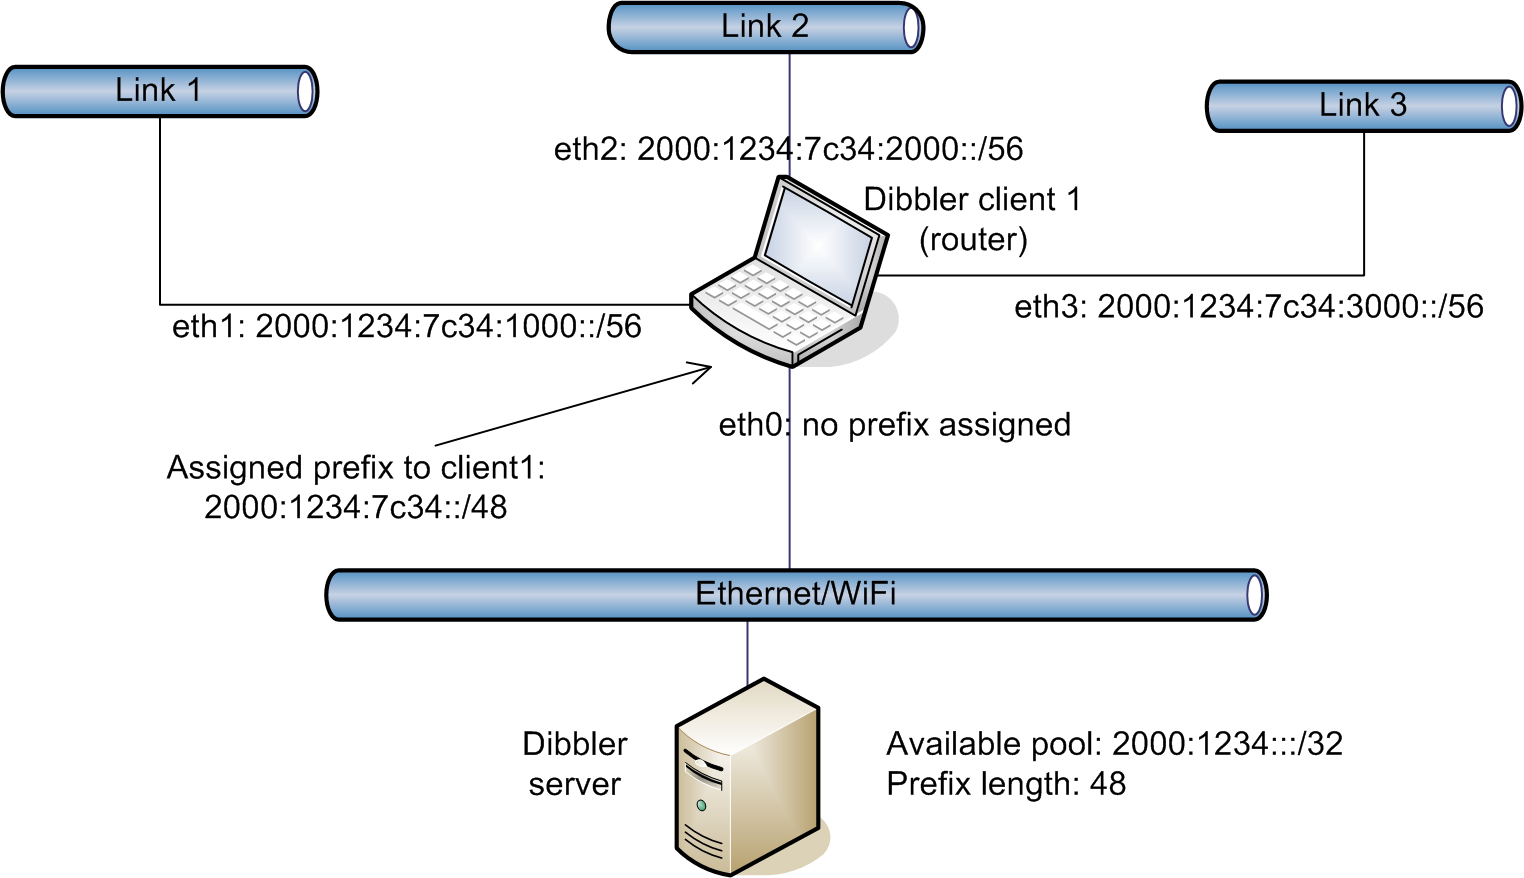
\includegraphics[width=0.65\textwidth]{dibbler-prefixes-router}
\caption{\emph{Prefix delegation (router behaviour)}}
\end{center}
\end{figure}

It is also possible to define multiple prefix pools. See section
\ref{example-server-prefix} for simple prefix delegation configuration
for server or section \ref{example-server-prefixes} for multiple
prefixes configuration. Also section \ref{example-client-prefix}
provides information related to client configuration.

\subsection{Relays}
\label{feature-relays}
In small networks, all nodes (server, hosts and routers) are connected
to the same network segment -- usually Ethernet segment or a single
access point or hotspot. This is very convenient as all clients can
reach server directly. However, larger networks usually are connected
via routers, so direct communication is not always possible. On the
other hand it is useful to have one server, which supports multiple
links -- some connected directly and some remotely.

\begin{figure}[ht]
\begin{center}
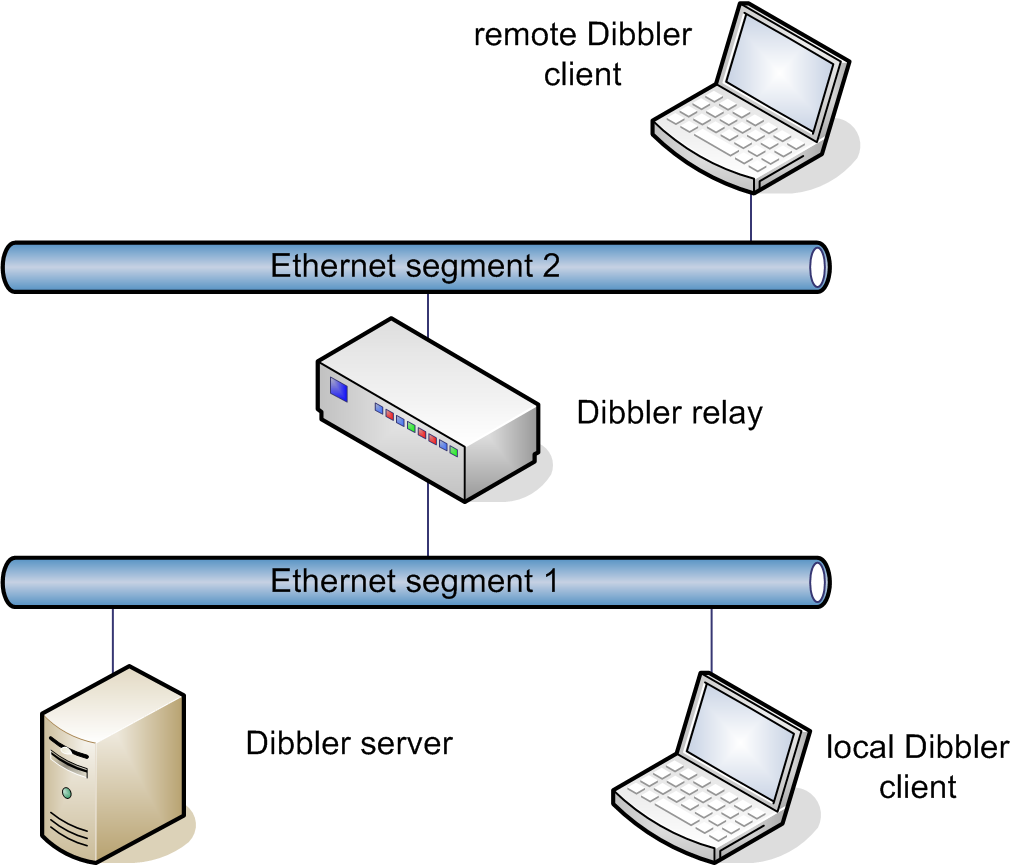
\includegraphics[width=0.65\textwidth]{dibbler-relay}
\caption{\emph{Relay deployment}}
\end{center}
\end{figure}

Very nice feature of the relays is that they appear as actual servers
from the client's point of view. Therefore no special arrangement or
configuration on the client side is required. On the other hand, from
the administrator point of view, it is much easier to manage one DHCPv6
server and deploy several relays than manage several servers on remote
links.

It is important to understand that relays not simply forward DHCPv6
messages. Each message forwarded from client to the server is
encapsulated. Also each message forwarded from server to a client is
decapsulated. Therefore additional server configuration is required to
deal with encapsulated (i.e. relayed) traffic.

To avoid confusion during reference to a specific link (i.e. eth0 on
the relay may be different link than eth0 on the server), each link
must be referred to using its unique interface-id. It is essential to 
use the same indentifier in the relay
configuration as well as in the server, so both will refer to the same
link using the same number. See section \ref{example-server-relay1} for
example how to configure server and section \ref{example-relay-1} for
corresponding relay configuration.

\begin{figure}[ht]
\begin{center}
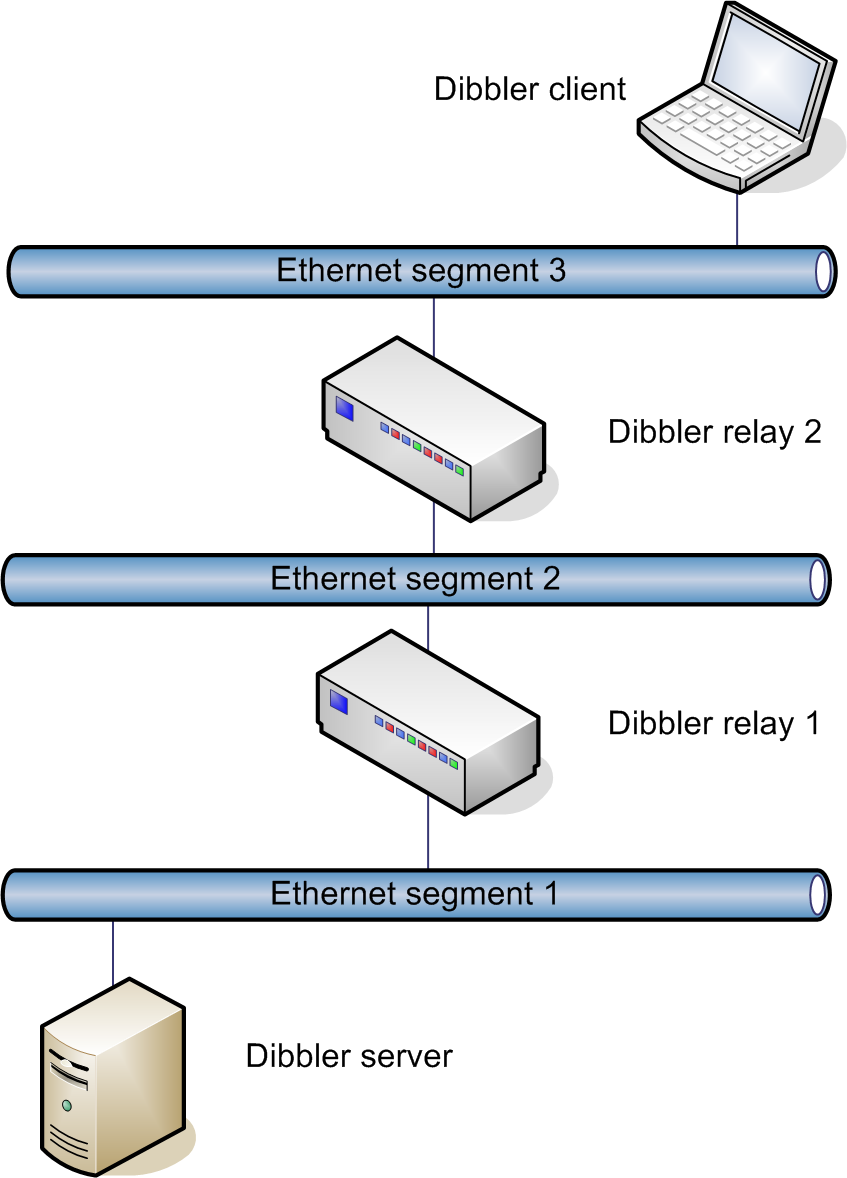
\includegraphics[width=0.4\textwidth]{dibbler-cascade-relays}
\caption{\emph{Cascade relays}}
\label{fig-cascade-relays}
\end{center}
\end{figure}

In larger networks it is sometimes useful to connect multiple
relays. Assuming there are 2 relays connecting server and client. Such
scenario is depicted on figure \ref{fig-cascade-relays}. Requests from
client are received by relay2, which encapsulates and sends them to
relay1. Relay1 further encapsulates those messages and sends them to
the server. Since server receives double encapsulated messages, it
must be properly configured to support such traffic. See section
\ref{example-server-relay2} for details about server configuration and
section \ref{example-relay-cascade} for example relays configuration.

\subsection{Address and prefix assignment policy}

Address and prefix assignment routines has been rewritten after 0.8.1
was released. It currently follows this algorithm:

\begin{enumerate}
\item Client classification is performed (a class is assigned to a client)
\item Client access control is performed (hosts listed on black-list are rejected,
  if any; if there is white-list defined, host must be on that list,
  otherwise it is rejected)
\item If existing lease this client/ia exists, it is assigned again
  (e.g. after host reboot)
\item Fixed lease is searched (using per-client configuration or so
  called exception mechanism). If found, this fixed lease is assigned.
\item max-client-leases is checked. If client already has maximum
  number of leases, further leases are declined.
\item Server checks if there is cached (i.e. previously assinged, but
  later released or expired) lease for this client. It is assigned, if
  possible.
\item Server checks if client sent any hints in SOLICIT or REQUEST
  message. Server tries to assign requested address or prefix. If this lease cannot be
  assinged for any reason, server tries to assign similar lease
  (i.e. from the same pool if client's hint was within supporte
  pool).
\item Otherwise, if all of above steps fails, server assigns a random
  address or prefix from supported pools.
\end{enumerate}

This algorithm is supported for non-temporary addresses and
prefixes. It is not supported for temporary addresses.

\subsection{Routing configuration}
\label{feature-routing}
Until recently, DHCPv6 protocol did not define a way to provision
routing configuration information to clients. The only way to deliver
this information to hosts was to use Router Advertisment mechanism in
Neighbor Discovery protocol \cite{rfc4862}. While that approach works,
it brings a number of drawbacks. In particular:
\begin{enumerate}
\item RA sent by router affects all hosts in a network. There is no
way to differentiate this information on a per host basis. There is no
way to define additional routing information for specified class of
hosts (e.g. one department in a corporate network).
\item RA and DHCPv6 configuration has to be consistent. That is very
doable, but somewhat problematic, because network configuration has to
be specified in several places. Moreover, it does not scale too
well. There are routers located in every segment of a network, while
there may be just a single DHCPv6 server deployed that serves many links.
\item Administrators experienced with IPv4 that are migrating their
networks to IPv6 ask this question very frequently: ``How do I
configure routing?''. Until recently the proper answer to that
question was ``you don't''.
\item In mobile environment, mobile nodes had to wait for RA and then
start DHCPv6 exchange. Although hosts can request RA by sending Router
Solicitation (RS), that may sometimes not work, as routers have upper
limits of how many RA they are allowed to sent.
\end{enumerate}

To solve aforementioned problems, a DHCPv6-based solution was
proposed \cite{draft-route-option}. It allows provisioning of IPv6
routing information. In particular, it allows configuration of a
default route, any reasonable number of specific routes and routes
available on link. This feature was introduced in Dibbler
0.8.1RC1. Both server and client support it. Dibbler sources come with
examples config files. See \verb+doc/example/server-route.conf+
and \verb+doc/example/client-route.conf+ for details. 

\Note This specification is not approved yet. It will change in the
future. In particular, IANA have not assigned specific option values
yet. Dibbler currently uses 242 for NEXT\_HOP and 243 for RTPREFIX
options. Those values will change.

\Note Current implementation is a prototype. It does support only one
route per router, only one router and only a single route
on-link. Although server is able to parse config that defines more
than one, it will provision only the first route or router information
to a client. That is implementation limitation that will be removed in
future releases. That is not a spec limitation.

To configure routing on a server side, following config may be used
\begin{lstlisting}
# Example server configuration file: server-route.conf

iface "eth0" {
# assign addresses from this pool
 class {
   pool 2000::/64
 }


# router with a single route with infinite lifetime
 next-hop 2001:db8:1::face:b00c {
     # replace this with ::/0 to configure default route
     route 2001:db8:1::/64
 }

# a single next-hop without any routes defined (i.e. default router)
# This simplified mode is recommended only in bandwidth restricted
# networks. Please use full mode instead
# next-hop 2001:db8:1::cafe

# router with 3 routes defined in different ways
 next-hop 2001:db8:1::dead:beef {
     # route may have defined a lifetime
     route 2001:db8:2::/64 lifetime 7200
     # lifetime may be infinite
     # route 2001:db8:3::/64 lifetime infinite
 }

# prefixes available on link directly, not via router
 route 2001:db8:5::/64 lifetime 3600
}
\end{lstlisting}

Support on client's side is enabled in a very simple way:
\begin{lstlisting}
# Example client configuration file: client-route.conf

# Uncomment following line to skip confirm sending (after crash or power outage)
skip-confirm

# 7 = omit debug messages
log-level 8

# Uncomment this line to run script every time response is received
script "/var/lib/dibbler/client-notify.sh"

iface "eth0" {
  ia

  option dns-server
  option domain
  routing 1
}
\end{lstlisting}

Two features should be enabled to reasonably use this
feature. \verb+routing 1+ instructs client that is should request routing
information (NEXT\_HOP and RTPREFIX options). Once such information is
sent by the server, client will execute a notify script. Client will
run defined script and pass necessary information to it. In
particular, it will set OPTION\_NEXT\_HOP, OPTION\_NEXT\_HOP\_RTPREFIX
and OPTION\_RTPREFIX variables with contents of received
option. Please see scripts/notify-scripts/client-notify.sh for example
on how to use that information to configure routing. User is also
recommended to read Section \ref{feature-script} about details of
running a script and passed variables.

\subsection{Custom options}
\label{feature-custom-options}
Dibbler is the DHCPv6 with support for a very large number of
options. However, there are always some new options that are not yet
supported. Another case is that vendors sometimes want to develop
and validate their private options before formal standarisation
process takes place. Starting with 0.8.0RC1, both client and server
are able to handle custom options. Even though author tries to
implement support for as many options as possible, there are always
cases, when that is not
enough. Some users may also test out new ideas, before thet get
standardized. Currently only several option layouts are supported, but
that list is going to be expanded. Server is able to support
following extra formats: generic (defined by hex string), IPv6
address, IPv6 address list and string (domain). To define those
options, use the following format:

\begin{lstlisting}
#server.conf
iface "eth0" {

 class {
   pool 2001:db8:1::/64
 }

 option 145 duid 01:02:a3:b4:c5:dd:ea
 option 146 address 2001:db8:1::dead:beef
 option 147 address-list 2001:db8:1::aaaa,2001:db8:1::bbbb
 option 148 string "secretlair.example.org"
}
\end{lstlisting}

Similar list can be configured for client. However, client can ask
for such custom options for testing purposes only, as mechanism for
handling those options once received is not yet implemented, as of
0.8.0RC1. Consider it experimental for the time being. Client can
request for an option using \opt{ORO} option or even send the option
in its messages.

Note that in 0.8.2 formatting of DUID-style options has
changed. ``DUID'' keyword is now required.

\begin{lstlisting}
#client.conf
iface "eth0" {
  unicast 1
  ia

  option 145 duid 01:02:a3:b4:c5:dd:ea
  option 146 address 2001:db8:1::dead:beef
  option 147 address-list 2001:db8:1::aaaa,2001:db8:1::bbbb
  option 148 string "secretlair.example.org"

  option 149 string request
  option 150 address request
  option 151 address-list request
\end{lstlisting}

A word of warning: There are no safety checks regarding option codes,
so it is possible to transmit already defined options using this
feature. Use with caution!

\subsection{DNS Update}
\label{feature-dns-update}
During normal operation, DHCPv6 client receives one or more IPv6
address(es) from DHCPv6 server. If configured to do so, it can also
receive information about DNS server addresses. As an additional
service, DNS Update can be performed. This feature, sometimes known as
Dynamic DNS, keeps DNS entries up to date. When client boots, it gets
its fully qualified domain name and this name can be used to reach
this particular client by other nodes. Details of this mechanism is
described in \cite{rfc4704}.

\Note In this section, we will assume that hostnames will be used from
the example.com domain and that addresses will be provided from the
2000::/64 pool.

\begin{figure}[ht]
\begin{center}
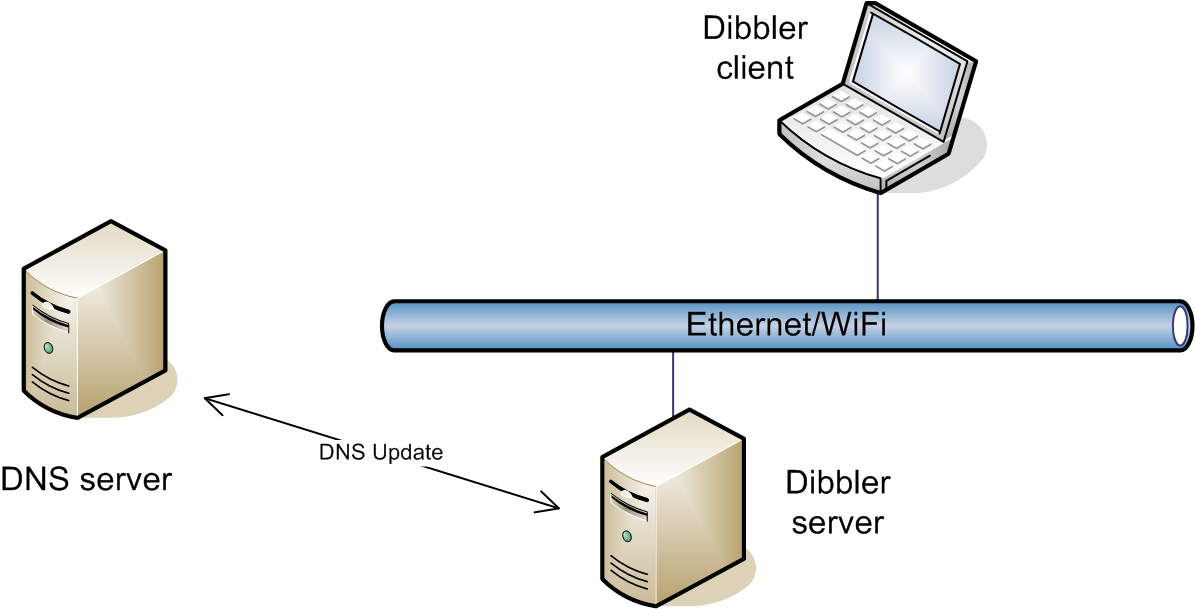
\includegraphics[width=0.65\textwidth]{dibbler-fqdn-srv-update}
\caption{\emph{DNS Update (performed by server)}}
\end{center}
\end{figure}

There are two types of the DNS Updates. First is a so called forward
resolving. It allows to change a node's name into its address,
e.g. malcolm.example.com can be translated into 2000::123. Other kind
of record, which can be updated is a so called reverse resolving. It
allows to obtain full name of a node with know address, e.g. 2000::124
can be translated into zoe.example.com.

To configure this feature, following steps must be performed:

\begin{enumerate}
\item Configure DNS server. DNS server supporting IPv6 and dynamic
  updates must be configured. One example of such server is an
  excellent \href{http://www.isc.org/software/bind}{ISC BIND}
  software. Version used during writing of this documentation was BIND
  9.7.2. It is necessary to allow listening on the IPv6 sockets and
  define that specific domain can be updated. See example below.
\item Configure Dibbler server to provide DNS server informations for
  clients. DNS Updates will be sent to the first DNS server on the
  list of available servers.
\item Configure Dibbler server to work in stateful mode, i.e. that it
  can provide addresses for the clients. This is a default mode, so
  unless configuration was altered, this step is already done. Make
  sure that there is no ,,stateless'' keyword in the
  \verb+server.conf+ file.
\item Define list of the available names in the server configuration
  file. Make sure to use fully qualified domain names
  (e.g. malcolm.example.com), not the hostnames only.
\item Configure dibbler client to request for DNS Update. Use ,,option
  fqdn'' to achieve this.
\item Server can be configured to execute
      \begin{itemize}
       \item both (AAAA and PTR) updates by itself
       \item execute PTR only by itself and let client execute AAAA
             update
       \item don't perform any updates and let client perform AAAA
             update.
      \end{itemize}
\end{enumerate}

Note that only server is allowed to perform PTR updates. After
configuration, client and/or server should log following line, which
informs that Dynamic DNS Update was completed successfully.

As of 0.8.0, both Dibbler server and client are using TCP connection
for DNS Updates. Connections are established over IPv6. There is no
support for IPv4 connections. Server uses first DNS server address
specified in \verb+dns-server+ option. It is possible to use
differentiate between DNS addresses provided to clients and the one
used for DDNS. To override DNS updates to be performed to different
address, use the following command:

\begin{lstlisting}
fqdn-ddns-address 2001:db8:1::1
\end{lstlisting}

\begin{figure}[ht]
\begin{center}
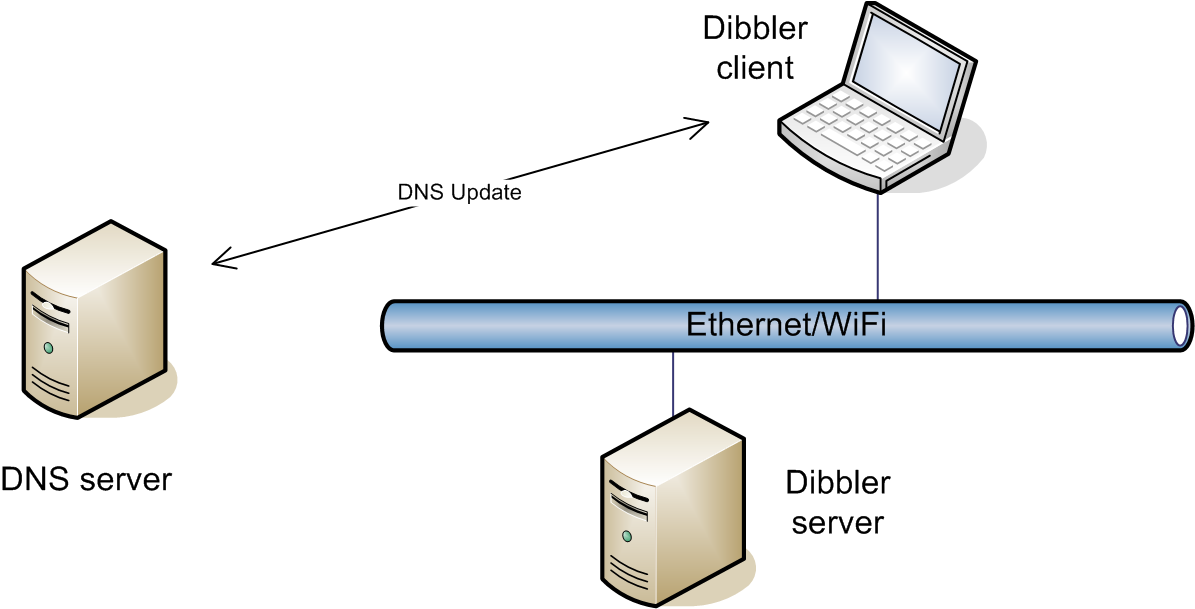
\includegraphics[width=0.65\textwidth]{dibbler-fqdn-cli-update}
\caption{\emph{DNS Update (performed by client)}}
\end{center}
\end{figure}

\subsubsection{Example BIND configuration}
Below are example configuration files for
the \href{http://www.isc.org/software/bind}{ISC BIND 9.7.2}, developed
by \href{http://www.isc.org}{Internet Systems Consortium, Inc.}.
First is a
relevant part of the /etc/bind/named.conf configuration file. Generally,
support for IPv6 in BIND is enabled (listen-on-v6) and there are two
zones added: example.com (normal domain) and
0.0.0.0.0.0.0.0.0.0.0.0.0.0.0.2.ip6.arpa (reverse
mapping). Corresponding files are stored in \verb+example.com+ and
\verb+rev-2000+ files. For details about meaning of those directives,
please consult \emph{BIND 9 Administrator Reference Manual}.

\Note Provided configuration is not safe from the security point of
view. See next subsection for details.

\begin{lstlisting}
// part of the /etc/bind/named.conf configuration file
options {
    listen-on-v6 { any; };
    listen-on    { any; };

    // other global options here
    // ...
};

zone "example.com" {
    type master;
    file "example.com";
    allow-update   { any; };
    allow-transfer { any; };
    allow-query    { any; };

    // other example.com domain-specific
    // options follow
    // ...
};

zone "0.0.0.0.0.0.0.0.0.0.0.0.0.0.0.2.ip6.arpa" {
    type master;
    file "rev-2000";
    allow-update   { any; };
    allow-transfer { any; };
    allow-query    { any; };

   // other 2000::/64 reverse domain related
   // options follow
   // ...
};
\end{lstlisting}

% \vspace{-0.3cm}
% \begin{center}
% BIND's named.conf example
% \end{center}

Below are examples of two files: forward and reverse zone. First example
presents how to configure normal domain. As an example there is entry
provided for zoe.example.com host, which has 2000::123 address. Note
that you do not have to manually configure such entries -- dibbler will
do this automatically. It was merely provided as an example, what kind
of mapping will be done in this zone.

\begin{lstlisting}
;
$ORIGIN .
$TTL 86400      ; 1 day
example.com             IN SOA  v13.klub.com.pl. root.v13.klub.com.pl. (
                                129        ; serial
                                7200       ; refresh (2 hours)
                                3600       ; retry (1 hour)
                                604800     ; expire (1 week)
                                86400      ; minimum (1 day)
                                )
                        NS      v13.klub.com.pl.
                        A       1.2.3.4
                        TXT     "Fake domain used for Dibbler tests."
$ORIGIN example.com.
$TTL 7200       ; 2 hours
zoe                     AAAA    2000::123
\end{lstlisting}

Second example presents zone file for reverse mapping. It contains
entries for a special zone called
0.0.0.0.0.0.0.0.0.0.0.0.0.0.0.2.ip6.arpa. This zone represents 2000::/64
address space. As an example there is a static entry, which maps address
2000::999 to a canonical name kaylee.example.com. Note that you do not
have to manually configure such entries -- dibbler will do this
automatically. It was merely provided as an example, what kind
of mapping will be done in this zone.

\begin{lstlisting}
; rev-2000 example file
$ORIGIN .
$TTL 259200     ; 3 days

; this line below is split in two due to page with limitation
0.0.0.0.0.0.0.0.0.0.0.0.0.0.0.2.ip6.arpa IN
      SOA 0.0.0.0.0.0.0.0.0.0.0.0.0.0.0.2.ip6.arpa. hostmaster.ep.net. (
; this line above is split in two due to page with limitation
                                200608268  ; serial
                                86400      ; refresh (1 day)
                                1800       ; retry (30 minutes)
                                172800     ; expire (2 days)
                                259200     ; minimum (3 days)
                                )
                        NS      klub.com.pl.
$ORIGIN 0.0.0.0.0.0.0.0.0.0.0.0.0.0.0.0.0.0.0.0.0.0.0.0.0.0.0.0.2.ip6.arpa.
$TTL 86200      ; 23 hours 56 minutes 40 seconds
3.2.1                   PTR     picard.example.com.

; this line below is split in two due to page with limitation
9.9.9                   PTR     kaylee.example.com.
$ORIGIN 0.0.0.0.0.0.0.0.0.0.0.0.0.0.0.2.ip6.arpa.

; example entry: 2000::999 -> troi.example.com.
; this line below is split in two due to page with limitation
9.9.9.0.0.0.0.0.0.0.0.0.0.0.0.0.0.0.0.0.0.0.0.0.0.0.0.0.0.0.0.2.ip6.arpa
      PTR troi.example.com.
; this line above is split in two due to page with limitation
\end{lstlisting}
\Note Due to page width limitation, if the example above, two lines were
split.
%% $

\subsubsection{Dynamic DNS Testing and tips}
Proper configuration of the DNS Update mechanism is not an easy
task. Therefore this section provides description of several methods of
testing and tuning BIND configuration. Please review following steps
before reporting issues to the author or on the mailing list.

\begin{itemize}
\item See example server and client configuration files described in a
  sections \ref{example-client-fqdn} and \ref{example-server-fqdn}.
  Also note that Dibbler distribution should be accompanied with
  several example configuration files. Some of them include FQDN usage
  examples.
\item Make sure that unix user, which runs BIND, is able to create and
  write file example.com.jnl. When BIND is unable to create this
  journal file, it will fail to accept updates from dibbler and will
  report failure. Check BIND log files, which are usually stored in
  the \verb+/var/log/+ directory.
\item Make sure that you have routing configured properly on a host,
  which will attempt to perform DNS Update. Use ping6 command to
  verify that DNS server is reachable from this host.
\item Make sure that your DNS server is configured properly. To do so,
  you might want to use \verb+nsupdate+ tool. It is part of the BIND
  distribution, but it is sometimes distributed separated as part of
  the dnsutils package. After executing nsupdate tool, specify address
  of the DNS server (\verb+server+ command), specify update parameters
  (\verb+update+ command) and then type \verb+send+. If nsupdate
  return a command prompt, then the update was successful. Otherwise
  nsupdate will print DNS server's response, e.g. NOTAUTH of
  SRVFAIL. See below for examples of successful forward (AAAA record)
  and reverse (PTR record) updates.
\item After DNS Update is performed, DNS records can be verified using
  dig command line tool (a part of the dnsutils package). Command
  syntax is: \verb+dig @(dns-server-address) name record-type+.  In
  the following example, this query checks for name jayne.example.com
  at a server located at 2000::1 address. Record type AAAA (standard
  record for resolving name into IPv6 address) is requested. dig tool
  provides server's response in the \verb+ANSWER SECTION:+. See
  example log below.
\item In example BIND configuration above, zone transfers, queries and
  updates are allowed from anywhere. To make this configuration more
  secure, it might be a good idea to allow updates only from a certain
  range of addresses or even one (DHCPv6 server's) address only.
\end{itemize}


%%%%%%%%%%%%%%%%%%%%%%%%%%%%%%%%%%%%%%%%%%%%%%%%%%%%%%%%%%%%%%%%%%%%%%%%%%%%%%%%

To manually make AAAA record update, type:
\begin{lstlisting}
nsupdate
>server 2000::1
>update add worf.example.com 7200 IN AAAA 2000::567
>send
\end{lstlisting}

To manually make PTR record update, type:
\begin{lstlisting}
nsupdate
>server 2000::1
>update add
3.2.1.0.0.0.0.0.0.0.0.0.0.0.0.0.0.0.0.0.0.0.0.0.0.0.0.0.0.0.0.2.ip6.arpa.
86200 IN PTR picard.example.com.
>send
\end{lstlisting}

\Note Everything between "update" and "picard.example.com" must be typed in one line.

And here is an example dig session:

\begin{lstlisting}
v13:/var# dig @2000::1 jayne.example.com AAAA
; <<>> DiG 9.3.2 <<>> @2000::1 jayne.example.com AAAA
; (1 server found)
;; global options:  printcmd
;; Got answer:
;; ->>HEADER<<- opcode: QUERY, status: NOERROR, id: 33416
;; flags: qr aa rd ra; QUERY: 1, ANSWER: 1, AUTHORITY: 1, ADDITIONAL: 2

;; QUESTION SECTION:
;jayne.example.com.             IN      AAAA

;; ANSWER SECTION:
jayne.example.com.      7200    IN      AAAA    2001::e4

;; AUTHORITY SECTION:
example.com.            86400   IN      NS      v13.klub.com.pl.

;; Query time: 6 msec
;; SERVER: 2000::1#53(2000::1)
;; WHEN: Mon Jul 24 01:38:13 2006
;; MSG SIZE  rcvd: 136
\end{lstlisting}
%% >>

\subsubsection{Accepting Unknown FQDNs}
By default, server configured to support FQDN has a list of names that
are to be provided to clients. But there are use cases, when client
uses its own name and sends it to the server. So it makes sense to
sometimes allow client's own domain names. Server does not know
anything about such names, thus its nickname "Unknown FQDN".

There are several actions that server can do, when unknown FQDN is
received. To configure such support for unknown FQDNs,
\verb+accept-unknonwn-fqdn+ option can be defined on an
interface. Depending on its, value, it may bave domain name as a parameter.
For example:

\begin{lstlisting}
iface "eth0" {

# assign addresses from this class
 class {
   pool 2000::/64
 }

# provide DNS server location to the clients
# also server will use this address to perform DNS Update,
# so it must be valid and DNS server must accept DNS Updates.
 option dns-server 2000::1

# provide their domain name
 option domain example.com

# provide fully qualified domain names for clients
# note that first, second and third entry is reserved
# for a specific address or a DUID

 option fqdn 1 64
             zebuline.example.com - 2000::1,
             kael.example.com - 2000::2,
             wash.example.com - 0x0001000043ce25b40013d4024bf5,
             zoe.example.com,
             malcolm.example.com,
             kaylee.example.com,
             jayne.example.com,
             inara.example.com

# specify what to do with client's names that are not on the list
# 0 - reject
# 1 - send other name from allowed list
# 2 - accept any name client sends
# 3 - accept any name client sends, but append specified domain suffix
# 4 - ignore client's hint, generate name based on his address, append domain name

 accept-unknown-fqdn 4 foo.bar.pl

}
\end{lstlisting}

\subsection{Introduction to client classification}
\label{feature-client-class}
It is possible to define more than one address class for a single
interface. Normally, when a client asks for an address, one of the
classes is being chosen on a random basis. If not specified otherwise,
all classes have equal probability of being chosen. However there are
cases where an Administrator wants to restrict access to a given pool
or to have distinct "client classes" associated to different address
pools. For example, Computer and IP-Telephone terminals can coexist in
the same LAN ; but the Computer must belong to given class pool
meanwhile the IP-Telephone must belong to another pool.

In order to implement the Client Class Classification, you must first
create the client class and then in the class declaration, indicate
which class to be allowed or denied. This point will be discussed in
detail in next sections.

\subsubsection{Client class  declaration}
Each client class used for class / ta / pd addressing must be defined
in the server configuration file at global scope. A client-class
declaration looks like this:

\begin{lstlisting}
Client-class TelephoneClass{
        match-if ( client.vendor-spec.en == 1234567)
}
\end{lstlisting}

Where TelephoneClass denotes the name of the client class and the
(client.vendor-spec.en == 1234567) denotes the condition an incoming
message shall match to belong to the Client-Class. The supported
operator and data will be discussed in next section.


\subsubsection{Access control}
Access control is based on a per pool basis. In the client-class
declaration; you can deny or allow the client class by using the
keyword "allow" or "deny". For example, following class accepts all
clients except those belonging to the client class "TelephoneClass":

\begin{lstlisting}
class {
     2000::/64
     deny TelephoneClass
}
\end{lstlisting}

Another example. This class accepts only client belonging to the
client class "TelephoneClass".

\begin{lstlisting}
class {
     2000::/64
     allow TelephoneClass
}
\end{lstlisting}

The rule can also be applied to TA/PD declaration. Several "allow"
directives can be associated to a given pool.

\begin{lstlisting}
ta-class {
     pool 2000::/64
     deny TelephoneClass
}

pd-class {
     pd-pool 2000::/80
     pd-length 96
     deny TelephoneClass
}
\end{lstlisting}

\subsubsection{Assigning clients to defined classes}
Classifying operators are used for assigning client to a specific class.
Currently, Dibbler supports the following Operators for classifying clients:

\begin{lstlisting}
Equal operator
    Syntax : ( Expr1 == Expr2 )
    Scope : global
    Purpose : returns "true" if Expr1 equals Expr2

And Operator
    Syntax : ( Condition1 and Condition2 )
    Scope : global
    Purpose : returns "true" if both Condition1 and Condition2 are "true"

Or operator
    Syntax : ( Condition1  or  Condition2 )
    Scope : global
    Purpose : returns "true" if either Condition1 or Condition2 is "true"

Contain Operator
    Syntax : ( String1 contain String2 )
    Scope : global
    Purpose :  returns "true" if String2 is a substring of String1

Substring Operator
    Syntax substring ( Expr1, index, length )
    Scope : global
    Purpose : returns the substring of the result of that evaluation
    that starts index characters from the beginning, continuing for
    length characters.
\end{lstlisting}

Dibbler accepts different data expressions -- or variables -- which
reflect value of options found in the packet to which the server is
responding.

\begin{description}
\item[client.vendor-spec.en] the enterprise number value of
  OptionVendorSpecific (OPTION\_VENDOR\_OPTS, option value equals to 17
  as per RFC3315)
\item[client.vendor-spec.data] the data of OptionVendorSpecific
  (OPTION\_VENDOR\_OPTS, option value equals to 17 as per RFC3315)
\item[client.vendor-class.en] the enterprise number value of
  OptionVendorClass (OPTION\_VENDOR\_CLASS, option value equal to 16 as
  per RFC3315)
\item[client.vendor-class.data] the data of OptionVendorClass
  (OPTION\_VENDOR\_CLASS, option value equals to 16 as per RFC3315)
\end{description}

\subsubsection{Examples of Client-Class Classifying}

Example 1 :
\begin{lstlisting}
Client-class CPEClass {
        match-if ( client.vendor-spec.data contain CPE )
}
\end{lstlisting}
Client belongs to CPEClass if its request message contains the Vendor
Specific option with the data field including the substring "CPE".


Example 2 : Combination with AND operator
\begin{lstlisting}
Client-class TelephoneClass {
  match-if (( client.vendor-spec.en == 1234) and ( client.vendor-spec.data contain CPE ) )
}
\end{lstlisting}

Example 3 : Combination with OR operator
\begin{lstlisting}
Client-class TelephoneClass {
  match-if (( client.vendor-spec.en == 1234) or ( client.vendor-spec.data contain CPE ) )
}
\end{lstlisting}

\subsection{External script}
\label{feature-script}

\Note Support for external scripts (often called \emph{notify script}
  was rewritten in 0.8.1RC1 release. Note that mapping prefix and
notify scripts were removed. Support for server-side script was
introduced in 0.8.1RC1.

Dibbler-client is able to receive addresses, prefixes and numerous
additional options. It will do its best to set up those parameters in
the system. However, the need for some extra processing may arise. The
most elegant solution is to call external script every time the
configuration changes. Dibbler client may be configured to call
external script every time REPLY is received for REQUEST (new
parameters added), RENEW (parameters were updated) or RELEASE
(parameters were deleted).

Name of this script is specified using \verb+script+ keyword followed
by absolute path to script. Script will be called with a single
parameter, denoting current operation. Its value will be one of
``add'', ``update'', ``delete'' or ``expire''. Currently ``expire''
event is triggered on server-side only. \footnote{Please send your
feedback to mailing list if you need it also on client-side.} Actual
values of received parameters are passed as environment variables. In
particular, IFNAME and IFINDEX variables denote interface name and
interface index that was used to communicate with server,
respectively. Another essential variable set is REMOTE\_ADDR. It
defines address from which packet originated. That is client's address
(when run on server) and server's address (when run on
client). Client's message type is passed in CLNT\_MESSAGE
variable. Server's response is passed in SRV\_MESSAGE. Note that
server's reply is most often REPLY as script execution is skipped after
sending ADVERTISE.

Addresses are passed in variables ADDR1, ADDR2 and following. Note
that each ADDR variable is accompanied with two additional variables:
ADDR1PREF (address preferred lifetime) and ADDR1VALID (address valid
lifetime). Prefixes are passed in variables PREFIX1, PREFIX2 and
following. Note that each PREFIX variable is accompanied with three
additional variales: PREFIX1LEN (prefix length), PREFIX1PREF (prefix
preferred lifetime), and PREFIX1VALID (prefix valid lifetime). Support
for additional options is in progress. Options are passed as
environment variables. For example client DUID (conveyed in option
code 1), will be passed as OPTION1.

To enable script execution, \verb+script+ global option must
be added to \verb+client.conf+ file. For example:

\begin{lstlisting}
# client.conf
script /var/lib/dibbler/script.sh

iface eth0 {
   ia
}
\end{lstlisting}

\subsection{Confirm}
\label{feature-confirm}
Client detects if previous client instance was not shutdown properly
(due to power outage, client crash, forceful shutdown or similar
event). In such case, it reads existing address database and checks if
assigned addresses may still be valid. If that is so, it tries to
confirm those addresses by using \msg{CONFIRM} message.

If you want to provoke this kind of scenario on purpose, you can run
dibbler-client normally, then forcefully kill the procss (by sending
kill -9 signal, or pressing ctrl-\\ under Linux). Make sure that you
rerun client before address valid lifetime expires.

Currently, client does support only IAs in the \msg{CONFIRM}.

\subsection{Mobility}
Client can also be compiled with support for link change detection.
The intended use for this feature is mobility. Client is able to
detect when it moves to new link and react accordingly. Client sends
\msg{CONFIRM} message to verify that its currently held address is
still usable on this new link.

\subsection{Leasequery}
\label{feature-leasequery}
Servers provide addresses, prefixes and other configuration options to
the clients. Sometime administrators may want to obtain information
regarding certain leases, e.g. who has been given a specific address
or what addresses have been assigned to a specific client. This
mechanism is called Leasequery \cite{rfc5007}. New DHCPv6 participant
called requestor has been defined. Its sole purpose is to send queries
and receive responses. Dibbler provides example implementation. To
define a query, command line parameters are used.

There are two types of queries: by address ("who leases this address?")
and by client identifier ("what addresses has this client?"). To specify
one of such types, \verb+-addr+ or \verb+duid+ command-line switches
can be used. It is also mandatory to specify (using \verb+-i IFACE+),
which interface should be used to transmit the query.

Here is a complete list of all command-line switches:

\begin{description}
\item[-i IFACE] -- defines thru which interface should the query be sent
\item[-addr ADDR] -- sets query type to query by address. Also defines
  address, which the query will be about.
\item[-duid DUID] -- sets query type to query by client
  indentifier. Also defines client intentifier.
\item[-timeout SECS] -- specifies time, which requestor should wait
  for response.
\item[-dstaddr ADDR] -- destination address of the lease query
  message. By default messages are sent to the multicast address
  (ff02::1:2). To transmit query to an unicast addres, use this option.
\end{description}

Example query 1: Who has 2000::1 address?

\begin{lstlisting}
dibbler-requestor -i eth0 -addr 2000::1
\end{lstlisting}

Example query 2: Which addresses are assigned to client with specific
client identifier?

\begin{lstlisting}
dibbler-requestor -i eth0 -duid 00:01:00:01:0e:8d:a2:d7:00:08:54:04:a3:24
\end{lstlisting}

\subsection{Stateless vs stateful and IA, TA options}
\label{feature-stateless-stateful}
This section explains the difference between stateless and stateful
configurations. IA and TA options usage is also described.

Usually, normal stateful configuration based on non-temporary
addresses should be used. If you don't know, what temporary addresses
are, you don't need them.

Note that DHCPv6 stateless autoconfiguration is part of stateless autoconfiguration
defined in \cite{rfc4862}.

There are two kinds of configurations in DHCPv6 (\cite{rfc3315},
\cite{rfc3736}):
\begin{description}
  \item[stateful] -- it assumes that addresses (and possibly other
    parameters) are assigned to a client. To perform this kind of
    configuration, four messages are exchanged: \msg{SOLICIT},
    \msg{ADVERTISE}, \msg{REQUEST} and \msg{REPLY}.
  \item[stateless] -- when only parameters are configured (without
    assigning addresses to a client). During execution of this type of
    configuration, only two messages are exchanged: \msg{INF-REQUEST}
    and \msg{REPLY}.
\end{description}

During normal operation, client works in a stateful mode. If not
instructed otherwise, it will request one or more normal
(i.e. non-temporary) address. It will use \opt{IA} option (Identity
Association for Non-temporary Addresses, see \cite{rfc3315} for
details) to request and retrieve addresses. Since this is a default
behavior, it does not have to be mentioned in the client configuration
file. Nevertheless, it can be provided:

\begin{lstlisting}
# client.conf
iface eth0 {
  ia
  option dns-server
}
\end{lstlisting}

In a specific circustances, client might be interested in obtaining
only temporary addresses. Although this is still a stateful mode, its
configuration is sligtly different. There is a special option called
\opt{TA} (Identity Association for Temporary Addresses, see
\cite{rfc3315} for details). This option will be used to request and
receive temporary addresses from the client. To force client to
request temporary addresses instead of permanent ones, \verb+ta+
keyword must be used in client.conf file. If this option is defined,
only temporary address will be requested. Keep in mind that temporary
addresses are not renewed.

\begin{lstlisting}
# client.conf
iface eth0 {
  ta
  option dns-server
}
\end{lstlisting}

It is also possible to instruct client to work in a stateless mode. It
will not ask for any type of addresses, but will ask for specific
non-adress related configuration parameters, e.g. DNS Servers
information. This can be achieved by using \verb+stateless+
keyword. Since this is a global parameter, it is not defined on any
interface, but as a global option.

\begin{lstlisting}
# client.conf
stateless
iface eth0
{
  option dns-server
}
\end{lstlisting}

Some of the cases mentioned above can be used together. However,
several combinations are illegal. Here is a complete list:

\begin{description}
\item[none] -- When no option is specified, client will assume one IA
  with one address should be requested. Client will send \verb+ia+
  option (stateful autoconfiguration).
\item[ia] -- Client will send \verb+ia+ option (stateful
  autoconfiguration).
\item[ia,ta] -- When both options are specified, client will request
  for both - Non-temporary as well as Temporary addresses (stateful
  autoconfiguration).
\item[stateless] -- Client will request additional configration
  parameters only and will not ask for addresses (stateless
  autoconfiguration).
\item[stateless,ia] -- This combination is not allowed.
\item[stateless,ta] -- This combination is not allowed.
\item[stateless,ia,ta] -- This combination is not allowed.
\end{description}

\subsection{Server address caching}
Previous Dibbler versions assigned a random address from the available
address pool, so the same client received different address each time it
asked for one. In the 0.5.0 release, new mechanism was introduced
to make sure that the same client gets the same address each time. It is
called \emph{Server caching}.

Below is the algorithm used by the server to assign an address to the client.

\begin{itemize}
 \item if the client provided hint, it is valid (i.e. is part of the
       supported address pool) and not used, then assign requested address.
 \item if the client provided hint, it is valid (i.e. is part of the
       supported address pool) but used, then assign free address from
       the same pool.
 \item if the client provided hint, but it is not valid (i.e. is not
       part of the supported address pool, is link-local or a multicast
       address), then ignore the hint completety.
 \item if the did not provide valid hint (or provided invalid one), try
       to assign address previously assigned to this client (address caching)
 \item if this is the first time the client is seen, assign any address
       available.
\end{itemize}
%% see SrvOptions/SrvOptIA_NA.cpp, TSrvOptIA_NA::getFreeAddr() method


\subsection{XML files}
\label{feature-xml}
During its execution, all dibbler components (client, server and
relay) store its internal information in the XML files. In Linux
systems, they are stored in the \verb+/var/lib/dibbler+ directory. In
Windows, current directory (i.e. directory where exe files are
located) is used instead. There are several xml files generated. Since
they are similar for each component, following list provides
description for server only:

\begin{itemize}
\item server-CfgMgr.xml -- Represents information read from a
  configuration file, e.g. available address pool or DNS server
      configuration.
\item server-IfaceMgr.xml -- Represens detected interfaces in the
  operating system, as well as bound sockets and similar information.
\item server-AddrMgr.xml -- This is database, which contains identity
  associations with associated addresses.
 \item server-cache.xml -- Since caching is implemented by the server
      only, this file is only created by the server. It contains
      information about previously assigned addresses.
\end{itemize}


\subsection{Authentication and Authorization}
\label{feature-auth}

Implementation of authentication and authorization in Dibbler is
loosely based on \cite{draft-aaa}. Mainly option formats have been
used, for interoperability purposes. This means that there should be
no reasonable expectation of interoperability with other
implementations.

Draft does not specify how to communicate with home and foreign AAA
servers (AAAH and AAAF) using Diameter or Radius protocol, so Dibbler
uses a different, simpler approach. Keys are stored locally in
files. (see Fig. \ref{fig-aaa}).

\begin{figure}[ht]
\begin{center}
\label{fig-aaa}
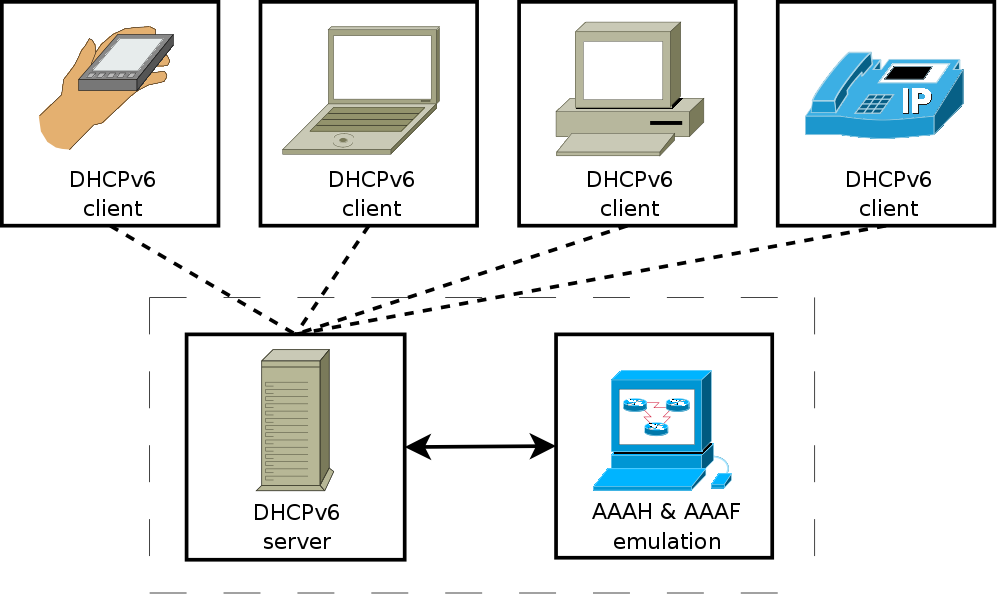
\includegraphics[width=0.65\textwidth]{dibbler-aaa}
\caption{\emph{Simplified model of AAA}}
\end{center}
\end{figure}

For each pair of client and server three files are needed. Client uses
a file \texttt{AAA-SPI}, which contains 32-bit AAA-SPI (AAA Security
Parameter Index) --- eight hexadecimal digits, to properly introduce
himself (authorize) to server. Also it needs file named
\texttt{AAA-key-\textit{AAASPI}}, which contains a key that is used to
generate authentication information in AAAAUTH and AUTH options. The
AAA-key is any number of arbitrary chosen bytes and is generated by
administrator of DHCPv6 server. The server needs only one file per
client to properly communicate using authentication. The file is named
\texttt{AAA-key-\textit{AAASPI}}, where \textit{AAASPI} is the same
value, that client has in \texttt{AAA-SPI} file. This file contains
the same AAA-key, that client has in \texttt{AAA-key} file. Dibbler
searches for those files in \textit{AAA directory}, which is
\texttt{/var/lib/dibbler/AAA} when running under Linux and current
directory, when running under Windows.

Typical scenario of preparing a client and server to use authentication:
\begin{enumerate}
 \item Administrator generates \texttt{AAA-key-\textit{AAASPI}}
   file. \textit{AAASPI} is an arbitrary chosen 32-bit number (as
   described above). The file contains any AAA-key and can be
   administrator's favorite poem or can be simply generated using
   \texttt{dd} and \texttt{/dev/urandom}:
\begin{lstlisting}
$ dd if=/dev/urandom of=AAA-key-b9a6452c bs=1 count=32
\end{lstlisting}
%%$

\item Administrator creates file \texttt{AAA-SPI} which contains
  previously chosen \textit{AAASPI}. This file will be used by the
  client only.

\item Administrator transfers \texttt{AAA-SPI} and
  \texttt{AAA-key-\textit{AAASPI}} to the client, using some secure
  method (e.g. mail+PGP, scp, https) to avoid sniffing the key by a
  potential attacker.

\item Client: User stores \texttt{AAA-SPI} and
  \texttt{AAA-key-\textit{AAASPI}} in \textit{AAA directory}.

\item Server: Administrator stores \texttt{AAA-key-\textit{AAASPI}} in
  \textit{AAA directory}.

\end{enumerate}

For example, configuration files can look like this:

\begin{itemize}
\item Server's \texttt{AAA-key-b9a6452c} and client's \texttt{AAA-key}
  (32 bytes):
\begin{lstlisting}
ma8s9849pujhaw09y4h[80pashydp80f
\end{lstlisting}

\item Client's \texttt{AAA-SPI} (8 bytes):
\begin{lstlisting}
b9a6452c
\end{lstlisting}
\end{itemize}

When configuration files are prepared and stored in client's and
server's \textit{AAA directory} you are ready to use
authentication. For detailed description of possible options see
\ref{client-conf-reference}. For quick start:
\begin{itemize}
 \item set ``\texttt{auth-enabled true}'' in \texttt{client.conf}

 \item set ``\texttt{auth-method digest-hmac-sha256}'' in
   \texttt{server.conf}

\end{itemize}

See section \ref{example-client-auth} for example client configuration
and \ref{example-server-auth} for server configuration.

\subsection{Exceptions: per client configuration}
\label{feature-exceptions}
All configuration parameters (except FQDN) are the same for all
clients, e.g. all clients will receive the same domain name and the
same DNS servers information.

However, it is sometimes useful to provide some clients with different
configuration parameters. For example computers from the accouting
department in a corporate network may be configured to be in a
different subdomain. Is is possible to specify that for particular
client different configuration options should be provided. Each client
is identified by its DUID. This mechanism is called \emph{per client
  configuration}, but it is sometimes referred to as
\emph{exceptions}. Support for per client prefix configuration has
been added in 0.8.2RC1.

See section \ref{example-server-exceptions} for server configuration
examples.

\subsection{Vendor specific information}
\label{feature-vendor-spec}
Dibbler supports vendor specific information options. As the name
suggests, that option is specific to a particular vendor. To be able
to support any vendor in a flexible manner, values are specified in a
hex format in \verb+server.conf+. For example:

\begin{lstlisting}
 option vendor-spec 1234-0x00002fedc
\end{lstlisting}

When client asks for a vendor-specific info, server will send
vendor-specific info option with enterprise number set to 1234 and
value option-data will be 00002fedc.

Although uncommon, it is also possible to specify multiple vendor
options. Another \verb+server.conf+ example:

\begin{lstlisting}
 option vendor-spec 1234-0x00002fedc,5678-0x0002aaaa
\end{lstlisting}

Server algorithm for choosing, which vendor option should be sent,
works as follows:

\begin{itemize}
\item When client requests for a speficic vendor (i.e. sends
  \opt{vendor-spec info} option with vendor field set), it will
  receive option for that specific vendor (i.e. requested 1234, got
  1234).
 \item When client requests any vendor (i.e. sends only \opt{option
   request} option with vendor-spec mentioned), it will receive first
   \opt{vendor-spec info} option from the list (i.e. 5678/0002aaaa).
 \item When client requests for not supported vendor (i.e. 11111), it
   will receive first vendor-spec option from the list
   (i.e. 5678/0002aaaa).
\end{itemize}

It is possible to configure Dibbler client to ask for vendor-specific
info. Granted value will not be used, so from the client's point of
view this feature may be used as testing tool for the server. Client
can request \opt{vendor-specific information} option in one of the
following ways:

\begin{description}
\item[option vendor-spec] -- Only \opt{option request} option will be
  sent with \opt{vendor-spec info} option mentioned.
\item[option vendor-spec 1234] -- \opt{option request} option will be
  sent with \opt{vendor-spec info} option mentioned, but also
  \opt{vendor-spec info} option with enterprise number set to 1234
  will be sent.
\item[option vendor-spec 1234 0x0a0b0c0d] -- \opt{option request}
  option will be sent with \opt{vendor-spec info} option mentioned,
  but also \opt{vendor-spec info} option with enterprise number set to
  1234 and option-data will be sent.
\end{description}

Although that is almost never needed, it is possible to configure
client to request multiple vendor-specific options at the same
time. That is also supported by the server. See
\ref{example-client-vendor-spec} for examples.


However, if client sends requests for multiple vendor-specific
options, which are not supported by the server, for each sent option,
server will assign one default vendor-spec option.

See \ref{example-client-vendor-spec} for client example and
\ref{example-server-vendor-spec} for server examples.

\subsection{Not connected interfaces (inactive-mode)}
\label{feature-inactive-mode}
During normal startup, client tries to bind all interfaces defined in
a configuration file. If such attempt fails, client reports an error
and gives up. Usually that is best action. However, in some cases it
is possible that interface is not ready yet, e.g. WLAN interface did
not complete association. Dibbler attempt to detect link-local
addresses, bind any sockets or initiate any kind of communication will
fail. To work around this disadvantage, a new mode has been
introduced in the 0.6.0RC4 version. It is possible to modify client
behavior, so it will accept downed and not running interfaces. To do
so, \emph{inactive-mode} keyword must be added to client.conf file. In
this mode, client will accept inactive interfaces, will add them to
inactive list and will periodically monitor its state. When the
interface finally goes on-line, client will try to configure it.

To test this mode, you can simulate deassociation using normal
Ethernet interface. Issue following commands:

\begin{itemize}
\item Bring down your interface (e.g. ifconfig eth0 down)
\item edit \verb+client.conf+ to enable inactive-mode
\item execute client: \verb+dibbler-client run+
\item client will print information related to not ready interface,
  and will periodically (once in 3 seconds) check interface state.
\item in a separate console, issue \verb+ifconfig eth0 up+ to bring
  the interface up.
\item dibbler-client will detect this and will initiate normal
  configuration process.
\end{itemize}

In the 0.6.1 version, similar feature has been introduced on the
server side. See sections \ref{example-client-inactivemode} and
\ref{example-server-inactivemode} for configuration examples.

\subsection{Parameters not supported by server (insist-mode)}
\label{feature-insist-mode}

Client can be instructed to obtain several configuration options, for
example DNS server configuration or domain name. It is possible that
server will not provide all requested options. Older versions of the
dibbler client had been very aggressive in such case. It tried very
hard to obtain such options. To do so, it did send \msg{INF-REQUEST}
to obtain such option. It is possible that some other DHCPv6 servers
will receive this message and will reply with valid configuration
parameters. This behavior has changed in the 0.6.0RC4 release. Right
now when client does not receive all requested options, it will
complain, but will take no action. To enable old behavior, so called
insist-mode has been added. To enable this mode, add
\verb+insist-mode+ at the global section of the \verb+client.conf+
file. Example configuration file is provided in the
\ref{example-client-insistmode}.

\subsection{Different DUID types}
\label{feature-duid-types}
There are 3 different types of the DUID (DHCP Unique Identifier):
\begin{itemize}
\item type 1 (link-layer + time) -- this DUID is based on Link-layer
  address and a current timestamp. According to spec \cite{rfc3315},
  that is a default type.
\item type 2 (enterprise number) -- this DUID is based on the Private
  Enterprise Number assigned to larger companies. Each vendor should
  maintain its own space of unique identifiers.
\item type 3 (link-layer) -- this DUID is based on link-layer address
  only.
\end{itemize}

According to spec \cite{rfc3315}, it is recommended to use link-layer
+ time, if possible. That DUID type provides most uniqueness. It has
one major drawback -- it is impossible to know DUID before it is
actually generated. That poses significant disadvantage to sysadmins,
who want to specify different configuration for each client. In such
cases, it is recommended to switch to link-layer only (type 3) DUIDs.

During first executing dibbler-client will generate its DUID and store
it in \verb+client-duid+ file on disk. During next startup DUID will
be read from the file, not generated.

It is possible to specify, what DUID format should be used. It is
worth noting that such definition is taken into consideration during
DUID generation only, i.e. during first client execution. To specify
DUID type, put only one of the following lines in the
\verb+client.conf+ file:

\begin{lstlisting}

# uncommend only ONE of the lines below
duid-type duid-llt
#duid-type duid-en 1234 0x56789abcde
#duid-type duid-ll

iface eth0 {
   ia
   option dns-server
}
\end{lstlisting}

When using link-layer+time or link-layer DUID types, dibbler will
autodetect addresses. To generate enterprise number-based DUID,
specific data must be provided: enterprise-number (a 32-bit integer,
1234 in the example above) and a enterprise-specific indentifier of
arbitrary length (56:78:9a:bc:de in the example above).

\subsection{Debugging/compatibility features}
During interoperability test session, it has been discovered that
sometimes various different implementations of the DHCPv6 protocol has
problem to interact with each other. As the protocol itself does not
specify all aspects and details, some things can ba done differently
and there is no only one ,,proper way''. It also happens that some
implementations may have problems with different than its authors
expected behaviors. To allow better interoperation between such
implementation, dibbler has some features, which cause different
behaviors. This could result in a successful operation with other
servers, clients and relays.

Normal users don't have to worry about those options, unless they are
using different servers, clients and relays. Those options also may be
useful for other vendors, who want to test their
implementations. Therefore those options can be perceived as a
debugging or testing features.

\subsubsection{Interface-id option}
During message relaying (done by relays), options can be placed in the
\msg{RELAY-FORW} message is arbitrary order. In general, there are two
options used: \opt{interface-id} option and \opt{relay-message}
option. The former defines interface identifier, which the original
data has been received from, while the later contains the whole
original message. When several relays are used, such message-in-option
encapsulation can occur multiple times.

It is possible to instruct relay to store \opt{interface-id} before
\opt{relay-message} option or after. There is also possibility to
instruct server to omit the \opt{interface-id} option altogether, but
since this violates \cite{rfc3315}, it should not be used. In general,
this configuration parameter is only useful when dealing with buggy
relays, which can't handle all option orders properly. Consider this
parameter a debugging feature.

Similar parameter is defined for the server. Server uses it during
\msg{RELAY-REPL} generation.

See description of the \emph{interface-id-order} parameters in Server
configuation (section \ref{server-conf}) and Relay configuration
(section \ref{relay-conf}).

\subsubsection{Non-empty IA\_NA option}
When client is interested in receiving an address, it sends
\opt{IA\_NA} option. In this option it may (but don't have to) include
addresses (using \opt{IAADDR} suboption) as hints for the server.

It has been detected that some servers does not support properly
(perfectly valid) empty \opt{IA\_NA} options. To work around this
problem, dibbler-client can be instructed to include two \opt{IAADDR}
in the \opt{IA\_NA} option. Here is minimal example config, which
achieves that:

\begin{lstlisting}
iface eth0 {
  ia {
     address
     address
  }
}
\end{lstlisting}

\subsubsection{Providing address/prefix hints}
Dibbler client can be instructed to send specific addresses or
prefixes in its \msg{SOLICIT} messages. This can be achieved by using
following syntax:
\begin{lstlisting}
# client.conf - request specific address/prefix
iface eth0 {
    ia {
        address { 2001:db8:dead:beef:: }
    }
    pd {
       prefix 2001:db8:aaaa::/64
    }
}
\end{lstlisting}

Be default, client will use those addresses in \msg{SOLICIT} message
only. When transmitting \msg{REQUEST} message, it will copy proposals
from \msg{ADVERTISE} message, received from a server. To force client
to use those specified addresses and/or prefixes also in
\msg{REQUEST}, please use \verb+insist-mode+ directive.

\subsection{Experimental features}

This section contains experimental features. Besides serving as a
general purpose DHCPv6 solution, dibbler is also used as a research
tool for new ideas. \footnote{This was particularly true during my
  Ph. D. research.} Normal users are recommended NOT to use any
of those features. Advanced users should take extra caution. Also be
aware that those options may not work as expected, may be incomplete
and not documented properly. You have been warned.

Since those mechanisms are non-standard, they are disabled by
default. To enable them, ,,experimental'' keyword must be placed in
the \verb+client.conf+ or \verb+server.conf+ files.

\subsubsection{Address Parameters}
\label{feature-addr-params}
\textbf{Note: This feature is experimental, i.e. it is not described
by any RFC or even internet draft. Don't use it, unless you exactly
know what you are doing.}

There is ongoing process to register and publish internet draft,
which describes this operation. Latest versions of this draft will be
availabe at \url{http://klub.com.pl/dhcpv6/doc/}.

RFC3315 (\cite{rfc3315}) defines means of allocating IPv6 addresses to
all interested clients. Clients are able to obtains IPv6 addresses and
other configuration parameters from the servers. Unfortunately, client
after obtaining an address, are not able to communicate each other due
to missing prefix information. That property of the DHCPv6 procotol is
sometimes perceived as a major disadvantage. To overcome this
deficiency, an extension to the protocol has been proposed.

It is possible to attach additional option conveyed in normal IAADDR
option. That additional option, called ADDRPARAMS option, contains
additional information related to that address. To maintain backward
compatibility, server does not send such option by default, even when
configured to support it. To make server send this option, client must
explicitly ask for it.

Below are example configuration files for server and client. Note that
since that is an non-standard feature, user must explicitly allow
experimental options before configuring it (thus ,,experimental''
keyword is required).

Example \verb+client.conf+ configuration file:

\begin{lstlisting}
#client.conf
log-mode short
log-level 8


iface "eth0" {
  ia {
     addr-params
  }
}
\end{lstlisting}

Example \verb+server.conf+ configuration file:

\begin{lstlisting}
#server.conf
log-level 8

experimental
log-mode short

iface eth0 {

 t1 60
 t2 96
 prefered-lifetime 120
 valid-lifetime 180

 class {
   addr-params 80
   pool 2001:458:ff01:ff03::/80
 }
}
\end{lstlisting}

\subsubsection{Remote Autoconfiguration}
\label{feature-remote-autoconf}
Every time a node attaches to a new link, it must renew or
obtain new address and parameters, using DHCPv6 protocol (namely
\msg{CONFIRM} or \msg{SOLICIT} messages.  In case of mobile nodes,
it is beneficial to obtain address and other  configuration parameters
remotely, before actually attaching to destination link.  This
extension provides experimental support for such operation.
Details of this mechanism are thoroughly discussed in \cite{phd,
  draft-remote-autoconf, networks2010, atnac2010}.

The idea is that once client attaches to its current location, normal
configuration procedure is initiated (\msg{SOLICIT}, \msg{ADVERTISE},
\msg{REQUEST} and \msg{REPLY}). However, besides requesting the usual
options, client also asks for \opt{NEIGHBORS} option. Server provides
that option that contains list of available DHCPv6 servers at
neighboring networks.

Once client gains that information, it then initiates remote
autoconfiguration process, i.e. it sends \msg{SOLICIT} message to each
of the newly discovered neighbors, requesting single IPv6
address. Servers respond remotely, using \msg{REPLY} message. Once
this exchange is completed, client knows its new IPv6 address for each
of the potential handover targets. What is especially important is
that client obtains that knowledge, while still being connected to old
location. It may leverage that knowledge, e.g. to update his
correspondent nodes in advance.

As Dibbler client is not a mobility software itself, it has to
communicate with Mobile IPv6 stack somehow. Therefore it triggers
./remote-autoconf script every time remote autoconfiguration is
concluded.

Note that to support this scenario, both client and all participating
servers must have unicast and rapid-commit support enabled.

Following series of server.conf files demonstrate, how 3 servers can
be configured to incorm client about their 2 neighbors.

\begin{lstlisting}
#server.conf for server1.
log-level 8
log-mode short
preference 2

experimental

iface "eth0" {

 t1 1800
 class {
   pool 2001:db8:1111::/64
 }

 rapid-commit 1
 unicast 2001:db8:1111::f

 option neighbors 2001:db8:2222::f,2001:db8:3333::f
}
\end{lstlisting}

\begin{lstlisting}
#server.conf for server2
log-level 8
log-mode short
preference 1

experimental

iface "eth1" {
 unicast 2001:db8:2222::f
 rapid-commit 1

 class {
   pool 2001:db8:2222::/64
 }


 option neighbors 2001:db8:1111::f,2001:db8:3333::f
}
\end{lstlisting}

\begin{lstlisting}
log-level 8
preference 0
experimental

iface "eth1" {

 unicast 2001:db8:3333::f
 rapid-commit 1
 class {
   pool 2001:db8:3333::/64
 }

 option dns-server 2001:db8:3333::f
 option neighbors 2001:db8:1111::f,2001:db8:2222::f
}
\end{lstlisting}

Client also needs to have enabled number of features. Following config
file may serve as an example:

\begin{lstlisting}
log-mode short
log-level 8

experimental
remote-autoconf

iface "eth0" {
  ia
  unicast 1
}
\end{lstlisting}

\subsection{Obsoleted experimental features}
This subsection describes experimental features that are not supported
anymore. This list is provided for historical reasons. It may be
useful for someone to ease tracking of features removal, e.g. to
get the latest version that still has support for something.

\subsubsection{Mapping prefix}
Mapping prefix was an extension that altered client's behavior when
delegated prefix is received. Instead of considering it as a prefix
that should be distributed on other interfaces, it is used as a mapping
prefix. Normal prefix processing is supressed and external script is
executed: \verb+mappingprefixadd+ or \verb+mappingprefixdel+. That
script must be present in the working directory (that would be
\verb+/var/lib/dibbler+ under Linux or current directory (Windows).
This feature was removed in 0.8.0RC1.

\subsubsection{Tunnel mode}
As support for DS-Lite \cite{rfc6334} support was added in
0.8.0RC1, the old support for configuring tunnels was removed.


%% CONFIG FILES
%%
%% Dibbler - a portable DHCPv6
%%
%% authors: Tomasz Mrugalski <thomson@klub.com.pl>
%%          Michal Kowalczuk <michal@kowalczuk.eu>
%%
%% released under GNU GPL v2 licence
%%

\newpage
\section{Server configuration}
\label{server-conf}
Server configuration is stored in \verb+server.conf+ file in the
\verb+/etc/dibbler+ (Linux systems) or in current (Windows systems)
directory.

\subsubsection{Global scope}
\label{server-global-scope}
Every option can be declared in a global scope. Global options can be
defined here. Also options of a smaller scopes can be defined here --
they will be used as a default values. Configuration file has following syntax:

\begin{lstlisting}
 global-options
 interface-options
 class-options
 interface-declaration
\end{lstlisting}

\subsubsection{Interface declaration}
\label{server-iface-scope}
Each network interface, which should be serviced by the server, must be
mentioned in the configuration file. Network interface is defined like this:
\begin{lstlisting}
iface interface-name
{
  interface-options
  class-options
}
\end{lstlisting}

or

\begin{lstlisting}
iface number
{
  interface-options
  class-options
}
\end{lstlisting}

where \verb+interface-name+ denotes name of the interface and
\verb+interface-number+ denotes its number. Name no longer needs to be
enclosed in single or double quotes (except Windows systems, when
interface name contains spaces). Note that virtual interfaces, used
to setup relay support are also declared in this way.

\subsubsection{Address class scope}
\label{server-class-scope}
Class is a smallest scope used in the server configuration file. It
contains definition of the addresses, which will be provided to
clients. Only class scoped parameters can be defined here. Address class
is declared as follows:
\begin{lstlisting}
class
{
  class-options
  address-pool
}
\end{lstlisting}

Address pool defines range of the addresses, which can be assigned to the
clients. It can be defined in one of the following formats:
\begin{lstlisting}
pool minaddress-maxaddress
pool address/prefix
\end{lstlisting}

\subsubsection{Prefix class scope}
\label{server-pd-class-scope}
That is an equivalent of address class for a prefix delegation. It
contains definition of prefixes that are going to be delegation to
clients. Only pd-class scoped parameters can be defined here. Prefix
class is declared as follows:
\begin{lstlisting}
pd-class
{
    pd-pool prefix/length
    pd-length prefix-length
}
\end{lstlisting}

\subsubsection{Temporary address class scope}
\label{server-ta-class-scope}
That is an equivalent of address class for temporary addresses. It
contains definition of temporary addresses that are going to be
assigned to clients that request temporary addresses. Only ta-class
scoped parameters can be defined here. Prefix class is declared as
follows: 
\begin{lstlisting}
ta-class {
    pool 2001:db8:1::1-2001:db81:1::ffff
}
\end{lstlisting}

\subsubsection{Routing scope}
\label{server-route-scope}
Support for routing configuration was added in 0.8.0RC1. It is
possible to define routing scope. Each scope represents a single
router available on-link. In this scope, routes available via
specified link my be defined.

\begin{lstlisting}
next-hop address-of-a-router
{
  route1-parameters
  route2-parameters
  ...
}
\end{lstlisting}

\subsubsection{Client scope}
\label{server-scope-client}
Server allows defining custom parameters on a per-host basis. See
Sections \ref{feature-exceptions} and \ref{example-server-exceptions} 
for details. There are two types of reservations: DUID-based and 
remote-id based. Following syntax can be used:

\begin{lstlisting}
client duid 00:00:00:00:00
{
    [address 2001:db8:1::]
    [prefix 2001:db8:1::/64]
    option1
    option2
    ...
}
\end{lstlisting}

\begin{lstlisting}
client remote-id 5-0x01020304
{
    [address 2001:db8:1::]
    [prefix 2001:db8:1::/64]
    option1
    option2
    ...
}
\end{lstlisting}

\subsubsection{Server options}

So called standard options are defined by the base DHCPv6 specification,
a so called RFC 3315 document \cite{rfc3315}. Those options are
called standard, because all DHCPv6 implementations, should properly
handle them. Each option has a specific scope it belongs to.

Standard options are declared in the following way:

\begin{lstlisting}
OptionName option-value
\end{lstlisting}

\begin{description}
\item[work-dir] -- (scope: global). Takes one parameter of string
  type. Defines working directory.

\item[log-level] -- (scope: global). Takes one integer
  parameter. Defines verbose level of the log messages. The valid range
  is from 1 (very quiet) to 8 (very verbose). Those values are modelled
  after levels used in syslog. These are: 1(Emergency), 2(Alert),
  3(Critical), 4(Error), 5 (Warning), 6(Notice), 7(Info) and
  8(Debug). Currently Dibbler is using levels 3 to 8, as 1 and 2 are
  reserved for system wide emergency events.

\item[log-name] -- (scope: global). Takes one string
  parameter. Defines than name, which will be used during logging.

\item[log-mode] -- (scope: global). Takes one parameter that can be
  short, full, precise or syslog. Defines logging mode. In the
  default, full mode, name, date and time in the h:m:s format will be
  printed. In short mode, only minutes and seconds will be printed
  (this mode is useful on terminals with limited width). Precise mode
  logs information with seconds and microsecond precision. It is a
  useful as a performance diagnostic tool for finding bottlenecks in
  the DHCPv6 autoconfiguration process. Syslog works under POSIX
  systems (Linux, Mac OS X, BSD family) and allows default POSIX
  logging functions.
  
\item[log-colors] -- (scope: global). Takes one boolean parameter.
  Defines if logs printed to console should use colors. That feature
  is used to enhance logs readability.  As it makes the log files
  messy on systems that do not support colors, it is disabled by
  default. The default is off.

 \item[cache-size] -- (scope: global). Takes one parameter that
  specifies cache size in bytes. The default value is 1048576
  (1MB). It defines a size of the memory (specified in bytes) which
  can se used to store cached entries.

\item[stateless] -- (scope: global). It may be present or missing. The
  default is missing. Defines that server should run in stateless
  mode. In this mode only configuration parameters are defined, not
  addresses or prefixes. It is mutually exclusive
  with \emph{class}, \emph{ta-class} and \emph{pd-class}. See
  Section \ref{feature-stateless-stateful}.


\item[interface-id-order] -- (scope: global). Take one parameter that
  can be one of \verb+before+, \verb+after+ or \verb+omit+. The
        default is \verb+before+. This parameter defines placement of
        the interface-id option. During message relaying options can
        be placed in the \msg{RELAY-REPL} message is arbitrary
        order. This option has been specified to control that
        order. \opt{interface-id} option can be placed before or
        after \opt{relay-message} option. There is also possibility to
        instruct server to omit the \opt{interface-id} option
        altogether, but since this violates \cite{rfc3315}, it should
        not be used. In general, this configuration parameter is only
        useful when dealing with buggy relays, which can't handle all
        option orders properly. Consider this parameter a debugging
        feature. Note: similar parameter is available in the
        dibbler-relay.

\item[experimental] -- (scope: global). Allows enabling experimental
features. There are some highly-experimental features present in
Dibbler. To make a clear statement about their experimental nature,
user is required to acknowledge that fact by putting this statement in
its config file. This statement may be present or absent. The default
is absent.

\item[inactive-mode] -- (scope: global, type: present or missing,
  default: missing). This enables so called inactive mode. When server
  begins operation and it detects that required interfaces are not
  ready, error message is printed and server exits. However, if
  inactive mode is enabled, server sleeps instead and wait for
  required interfaces to become operational. That is a useful feature,
  when using wireless interfaces, which take some time to initialize
  as associate.

\item[accept-leasequery] -- (scope: interface). Takes one boolean
  parameter that specifies if server should support leasequery
  \cite{rfc5007} protocol on a given interface. The default value is
  0 (leasequery is not supported by default). See Section
  \ref{feature-leasequery}.

%%% TODO bulk-leasequery-accept
%%% TODO bulk-leasequery-tcp-port
%%% TODO bulk-leasequery-max-conns
%%% TODO bulk-leasequery-timeout

\item[guess-mode] -- (scope: global, type: present or missing,
  default: missing). When this option is enabled, server will not pay
  close attention to the interface-id option in relayed messages. If
  interface-id has a value other than specified in server.conf or even
  when there is no interface-id option at all, it will use first relay
  defined.

\item[script] -- (scope: global). Takes one string parameter that
  specifies name of a script that will be called every time something
  important happens in a system, e.g. when address or prefix is
  assigned, updated or released. See Section \ref{feature-script}.

\item[fqdn-ddns-address] -- (scope: global). Takes one parameter that
  specifies address of DNS server that will be used for DNS
  Updates. See Section \ref{feature-dns-update}.

\item[ddns-protocol] -- (scope: global). Takes one string
parameter. Defines protocol that should be used during DNS Update
mechanism. Allowed values are \verb+tcp+, \verb+udp+ and \verb+any+.
Any means that UDP will be tried first and if it fails, update will be
retried over TCP. See Section \ref{feature-dns-update}.

\item[ddns-timeout] -- (scope: global). Takes one integer parameter
that specifies timeout in milliseconds. Defines how long client should
wait for DNS server response during DNS Update before declaring
update a failure. See Section \ref{feature-dns-update}.

\item[class] -- (scope: interface). This definition must be followed by
curly braces and creates a new address class scope. See
Section \ref{server-class-scope}.

\item[pd-class] -- (scope: interface). This definition must be
followed by curly braces and creates a new prefix-delegation class
scope. See Section \ref{server-pd-class-scope}.

\item[ta-class] -- (scope: interface). This definition must be
followed by curly braces and creates a new temporary address class
scope. See Section \ref{server-ta-class-scope}.

\item[next-hop] -- (scope: interface). This definition takes one
parameter that defines IPv6 address of a router. Without any further
parameters, it conveys an information about default route for
bandwidth limited networks. That mode is discouraged, unless there are
significant bandwith limitations. It is usually followed by curly
braces that create a new route scope. See Section \ref{server-route-scope}.

 \item[preference] -- (scope: interface, type: 0-255, default:
            none). Eech server can be configured to a specific
            preference level. When client receives several
            \msg{ADVERTISE} messages, it should choose that server,
            which has the highest preference level. It is also worth
            noting that client, upon reception of the \msg{ADVERTISE}
            message with preference set to 255 should skip wait phase
            for possible other \msg{ADVERTISE} messages.


 \item[unicast] -- (scope: interface, type: address,
            default:none). Normally clients sends data to a well known
            multicast address. This is easy to achieve, but it wastes
            network resources as all nodes in the network must process
            such messages and also network load is increased. To prevent
            this, server might be configured to inform clients about its
            unicast address, so clients, which accept it, will switch to
            a unicast communication.

 \item[rapid-commit] -- (scope: interface, type: boolean, default:
            0). This option allows rapid commit procedure to be
            performed. Note that enabling rapid commit on the server
            side is not enough. Client must be configured to allow
            rapid commit, too.

\item[iface-max-lease] -- (scope: interface, type: integer, default:
            $2^{32}-1$). This parameter defines, how many normal
            addresses can be granted on this interface.

\item[client-max-lease] -- (scope: interface, type: interger,
            default:$2^{32}-1$). This parameter defines, how many
            addresses one client can get. Main purpose of this
            parameter is to limit number of used addresses by
            misbehaving (malicious or restarting) clients.

\item[relay] -- (scope: interface). Takes one string or integer
  parameter that designated interface name or interface index. It is
  used in relay definition.  It specifies name of the physical (or
  name of another relay, if cascade relaying is used) interface, which
  is used to receive and transmit relayed data. See
  \ref{feature-relays} for details of relay deployment and sections
  \ref{example-server-relay1} and \ref{example-server-relay2} for
  configuration examples.

\item[interface-id] -- (scope: interface, type: integer, default: not
  defined). Used in relay definition. Each relay interface should have
  defined its unique identified. It will be sent in the
  \opt{interface-id} option. Note that this value must be the same as
  configured in the dibbler-relay. It may be possible to specify this
  parameter by using a number (option will be 4 bytes long), a string
  or a hex of arbitrary length (please use the same format as for
  DUID). See \ref{feature-relays}, \ref{example-server-relay1} and
  \ref{example-relay} for details.

 \item[vendor-spec] -- (scope: interface, type: integer-hexstring,
   default: not defined). This parameter can be used to configure some
   vendor-specific information option. Since there are no
   dibbler-specific options, this implementation is flexible. User can
   specify in the configuration file, how should this option look
   like. See \ref{example-server-vendor-spec} section for details. It
   is uncommon, but possible to define several vendor specific options
   for different vendors. In such case, administrator must specify
   coma separated list. Each list entry is a vendor (enterprise
   number), ,,--'' sign and a hex dump (similar to DUID).

 \item[pool] -- (scope: class). Takes coma separated IPv6 address
   ranges. Each range is defined as first-address, a dash and a second
   address. Defines a range of available addresses that will be
   assigned in specific class. An example pool definition looks like
   this:
   \begin{lstlisting}
     pool 2001:db8:abcd:: - 2001:db8:abcd::ffff
   \end{lstlisting}
   It is also possible to use prefix/length notation.

 \item[pd-pool] -- (scope: pd-class). Takes coma separated IPv6
   address ranges. Each range is defined as fist-address, a dash and a
   second address. Defines a range of available prefixes (only
   prefixes themselves, not their lengths) that will be assigned in
   specific class. An example pd-pool definition looks like this:
   \begin{lstlisting}
     pd-pool 2001:db8:abcd:: - 2001:db8:abcd::ffff
   \end{lstlisting}
   It is also possible to use prefix/length notation.

\item[share] -- (scope: class). Defines percentage of clients that a
  class should handle. This parameter is only useful if there are more
  then one class defined. See Section
  \ref{example-server-multiple-classes}.

 \item[T1] -- (scope: class, type: integer or integer range: default:
   $2^{32}-1$). This value defines after what time client should start
   renew process. Exact value or accepted range can be specified. When
   exact value is defined, client's hints are ignored completely.

 \item[T2] -- (scope: class, type: integer or integer range,
   default:$2^{32}-1$). This value defines after what time client will
   start emergency rebind procedure if renew process fails. Exact
   value or accepted range can be specified. When exact value is
   defined, client's hints are ignored completely.

\item[valid-lifetime] (scope: class, type: integer or integer range,
            default:$2^{32}-1$). This parameter defines valid lifetime of
            the granted addresses. If range is specified, client's
            hints from that range are accepted.

\item[preferred-lifetime] (scope: class, type: integer or integer range,
            default:$2^{32}-1$). This parameter defines prefered
            lifetime of the granted addresses. If range is specified,
            client's hits from that range will be accepted.

\item[class-max-lease]  -- (scope: interface, type: interger,
            default:$2^{32}-1$). This parameter defines, how many
            addresses can be assigned from that class.

\item[reject-clients] -- (scope: class, type: address or DUID list,
            default: none). This parameter is sometimes called
            black-list. It is a list of a clients, which should not be
            supported. Clients can be identified by theirs link-local
            addresses or DUIDs.

\item[accept-only] -- (scope: class, type: address or DUID list,
            default: none). This parameter is sometimes called
            white-list. It is a list of supported clients. When this
            list is not defined, by default all clients (except
            mentioned in reject-clients) are supported. When
            accept-only list is defined, only client from that list
            will be supported.

\item[addr-params] -- (scope: class). Experimental feature that takes 
  one boolean parameter. It defines prefix length that is configured
  in addr-params option. See Section \ref{feature-addr-params}.

\item[allow] -- (scope: class). Specifies that clients that belong to
  a specific client class are allowed to use that address class. Takes
  one string parameter that defines client class name. See Section
  \ref{feature-client-class}.

\item[deny] -- (scope: class). Specifies that clients that belong to
  a specific client class are denied use of that address class. Takes
  one string parameter that defines client class name. See Section
  \ref{feature-client-class}.

 \item[option dns-server] -- (scope: interface, type: address list, default:
   none). This option conveys information about DNS servers
   available. After retriving this information, clients will be able
   to resolve domain names into IP (both IPv4 and IPv6)
   addresses. Defined in \cite{rfc3596}.

 \item[option domain] -- (scope: interface, type: domain list, default:
   none). This option is used for configuring one or more domain
   names, which clients are connected in. For example, if client's
   hostname is \verb+alice.mylab.example.com+ and it wants to contact
   \verb+bob.mylab.example.com+, it can simply refer to it as
   \verb+bob+. Without domain name configured, it would have to use
   full domain name. Defined in \cite{rfc3596}.

 \item[option ntp-server] -- (scope: interface, type: address list, default:
   none). This option defines information about available NTP
   servers. Network Time Protocol \cite{rfc2030} is a protocol used
   for time synchronisation, so all hosts in the network has the same
   proper time set. Defined in \cite{rfc4075}.

 \item[option time-zone] -- (scope: interface, type: timezone, default:
   none). It is possible to configure timezone, which is provided by
   the server. Note that this option is considered obsolete as it is
   mentioned in draft version only \cite{draft-timezone}. Work on this
   draft seems to be abandoned as similar functionality is provided by
   now standard \cite{rfc4075}.

 \item[option sip-server] -- (scope: interface, type: address list, default:
   none). Session Initiation Protocol \cite{rfc3263} is an control
   protocol for creating, modifying, and terminating sessions with one
   or more participants. These sessions include Internet telephone
   calls, multimedia distribution, and multimedia conferences. Its
   most common usage is VoIP. Format of this option is defined in
   \cite{rfc3319}.

 \item[option sip-domain] -- (scope: interface, type: domain list, default:
   none). It is possible to define domain names for Session Initiation
   Protocol \cite{rfc3263}. Configuration of this parameter will ease
   usage of domain names in the SIP protocol. Format of this option is
   defined in \cite{rfc3319}.

 \item[option nis-server] -- (scope: interface, type: address list, default:
   none). Network Information Service (NIS) is a Unix-based system
   designed to use common login and user information on multiple
   systems, e.g. universities, where students can log on to ther
   accounts from any host. Its format is defined in \cite{rfc3898}.

 \item[option nis-domain] -- (scope: interface, type: domain list, default:
   none). Network Information Service (NIS) can albo specify domain
   names. It can be configured with this option. It is defined in
   \cite{rfc3898}.

 \item[option nis+-server] -- (scope: interface, type: address list, default:
   none). Network Information Service Plus (NIS+) is an improved
   version of the NIS protocol. This option is defined in
   \cite{rfc3898}.

 \item[option nis+-domain] -- (scope: interface, type: domain list, default:
   none). Similar to nis-domain, it defines domains for NIS+. This
   option is defined in \cite{rfc3898}.

 \item[option lifetime] -- (scope: interface, type: boolean, default:
   no). Base spec of the DHCPv6 protocol does offers way of refreshing
   addresses only, but not the options. Lifetime defines, how often
   client should renew all its options. When defined, lifetime option
   will be appended to all replies, which server sends to a client. If
   client does not support it, it should ignore this option. Format of
   this option is defined in \cite{rfc4242}.

 \item[option fqdn] -- (scope: interface). Takes 0, 1 or 2 integer
   parameters that are followed by FQDN list. Additional integer
   parameters designate fqdn-mode and reverse zone length in DNS
   Update. FQDN-mode can have 3 values: 2 (both AAAA and PTR record
   will be updated by server), 1 (server will update PTR only) or 
   0 (server will not update anything). Reverse zone length is an
   integer between 0 and 128 and designates reverse zone length. FQDN
   list is a coma separated list of fully qualified domain names, with
   possible reservations for DUIDs or addresses. FQDN mechanism is
   defined in \cite{rfc4704}. See Section \ref{feature-dns-update}.
   
\item[accept-unknown-fqdn] -- (scope: Interface). Takes one integer
  parameter, possibly followed by second string parameter that
  designated domain name. It specifies how server should react to
  incoming FQDN options that contain names that are unknown to the
  server. Allowed values are 0 (reject), 1 (send other name from
  allowed list), 2 (accept any name client sends), 3(accept any name
  client sends, but append specified domain suffix) and 4 (ignore
  client's hint, generate name based on his address, append domain
  name). Choices 3 and 4 require additional string parameter that
  defines domain suffix. See Sections \ref{feature-dns-update}
  and \label{example-server-fqdn}.
 
\item[option] -- (scope: interface). Takes one integer number followed
  by several possible parameter combinations. It defines custom
  option that server may send out to clients. Supported formats are:
  \begin{lstlisting}
    option number - DUID
    option number address-keyword address
    option number address-list
    option number string-keyword string
  \end{lstlisting}
Where number is an integer that defined option type, DUID is a
hex-formatted string that defines option content, address-keyword is a
word ``address'', address is an IPv6 address, address-list is coma
separated list of addresses, string-keyword is a word ``string'' and
string is any string enclosed in single or double quotes. See Section
\ref{feature-custom-options} and \ref{example-server-custom}.

 \item[option aftr] -- (scope: interface, type: FQDN). In Dual-Stack Lite
   networks, client may want to configure DS-Lite tunnel. Client may
   want to obtain information about AFTR (a remote tunnel
   endpoint). This option conveys a fully qualified domain name of the
   remote tunnel. This option is defined in \cite{rfc6334}.

 \item[option neighbors] -- (scope: interface). Experimental feature
   for Remote Autoconfiguration. Do not use it unless you know exactly
   what you are doing. Takes coma separated list of addresses. This
   option requires \emph{experimental} mode to be enabled. See Section
   \ref{feature-remote-autoconf}.

 \item[auth-method] -- (scope: global, type: string, default:
   empty). Set it to one of the following values to enable
   authentication on ther server side, using selected method of
   generating authentication information:
   \texttt{none}, \texttt{digest\_plain}, \texttt{digest\_hmac\_md5},
   \texttt{digest\_hmac\_sha1}, \texttt{digest\_hmac\_sha224},
   \texttt{digest\_hmac\_sha256}, \texttt{digest\_hmac\_sha384},
   and \texttt{digest\_hmac\_sha512}.

 \item[auth-lifetime] -- (scope: global, type: integer, default:
   0). Authentication lifetime. Currently not supported.

 \item[auth-key-len] -- (scope: global, type: integes, default:
   32). Key generation nonce length (see \cite{draft-aaa} for
   details).

\item[client-class] -- (scope: global). Takes one string parameter
  that defines name of a client class. Client class name is followed
  by curly brackets that create client-class scope. Clients can be
  grouped into classes depending on rules defined in
  client-class. This can be used together with \verb+allow+ and
  \verb+deny+ to assign segregate clients into different groups. See
  Section \ref{feature-client-class} for overview and Section
  \ref{class-expressions} for list of supported expressions.

\item[address] -- (scope: client). Takes one parameter that specifies
   address. It instructs server to reserve this particular address for
   defined client. See Sections \ref{feature-exceptions}
   and \ref{example-server-exceptions} for details.

\item[prefix] -- (scope: client). Takes one parameter that specifies
   prefix using prefix/length notation. It instructs server to reserve
   specified prefix for defined client. See Sections \ref{feature-exceptions}
   and \ref{example-server-exceptions} for details.

\end{description}

\subsubsection{Client class quantifiers}
\label{class-expressions}
Additional parameters are used during client class definition. See
Section \ref{feature-client-class} for details and examples.

\begin{description}
\item[match-if] -- (scope: client-class). 
\item[contain] -- (scope: client-class).
\item[substring] -- (scope: client-class).
\item[==] -- (scope: client-class).
\item[and] -- (scope: client-class).
\item[or] -- (scope: client-class).
\item[client.vendor-spec.en] -- (scope: client-class).
\item[client.vendor-spec.data] -- (scope: client-class).
\item[client.vendor-class.en] -- (scope: client-class).
\item[client.vendor-class.data] -- (scope: client-class).
\end{description}


\subsection{Server configuration examples}

This subsection contains various examples of the server
configuration. If you are interested in additional examples, download
source version and look at \verb+*.conf+ files.

\subsubsection{Example 1: Simple}

In opposite to client, server uses only interfaces described in config
file. Let's examine this common situation: server has interface named
\emph{eth0} (which is fourth interface in the system) and is supposed
to assign addresses from 2000::100/124 class. Simplest config file
looks like that:

\begin{lstlisting}
# server.conf
iface eth0
{
  class
  {
    pool 2000::100-2000::10f
  }
}
\end{lstlisting}

\subsubsection{Example 2: Timeouts}
Server should be configured to deliver specific timer values to the
clients. This example shows how to instruct client to renew (T1 timer)
addresses one in 10 minutes. In case of problems, ask other servers in
15 minutes (T2 timer), that allowe prefered lifetime range is from 30
minutes to 2 hours, and valid lifetime is from 1 hour to 1 day. DNS
server parameter is also provided. Lifetime option is used to make
clients renew all non-address related options renew once in 2 hours.

\begin{lstlisting}
# server.conf
iface eth0
{
  T1 600
  T2 900
  prefered-lifetime 1800-3600
  valid-lifetime 3600-86400
  class
  {
    pool 2000::100/80
  }

  option dns-server 2000::1234
  option lifetime 7200
}
\end{lstlisting}

\subsubsection{Example 3: Limiting amount of addresses}
Another example: Server should support 2000::0/120 class on eth0
interface. It should not allow any client to obtain more than 5
addresses and should not grant more then 50 addresses in total. From
this specific class only 20 addresses can be assigned. Server
preference should be set to 7. This means that this server is more
important than all server with preference set to 6 or less.
Config file is presented below:

\begin{lstlisting}
# server.conf
iface eth0
{
  iface-max-lease 50
  client-max-lease 5
  preference 7
  class
  {
    class-max-lease 20
    pool 2000::1-2000::100
  }
}
\end{lstlisting}

\subsubsection{Example 4: Unicast communication}
\label{example-server-unicast}

Here's modified previous example. Instead of specified limits, unicast
communication should be supported and server should listen on
2000::1234 address. Note that default multicast address is still
supported. You must have this unicast address already configured on
server's interface.

\begin{lstlisting}
# server.conf
log-level 7
iface eth0
{
  unicast 2000::1234
  class
  {
    pool 2000::1-2000::100
  }
}
\end{lstlisting}

\subsubsection{Example 5: Rapid-commit}
This configuration can be called quick. Rapid-commit is a way to shorten exchange to only two messages. It is
quite useful in networks with heavy load. In case if client does not
support rapid-commit, another trick is used. Preference is set to
maximum possible value. 255 has a special meaning: it makes client to
skip wait phase for possible advertise messages from other servers and
quickly request addresses.

\begin{lstlisting}
# server.conf
log-level 7
iface eth0
{
  rapid-commit yes
  preference 255
  class
  {
    pool 2000::1/112
  }
}
\end{lstlisting}

\subsubsection{Example 6: Access control}
Administrators can selectively allow certain client to use this
server (white-list). On the other hand, some clients could be
explicitly forbidden to use this server (black-list). Specific DUIDs,
DUID ranges, link-local addresses or the whole address ranges are
supported. Here is config file:

\begin{lstlisting}
# server.conf
iface eth0
{
  class
  {
    # duid of the rejected client
    reject-clients ``00001231200adeaaa''
    2000::2f-2000::20  // it's in reverse order, but it works.
                       // just a trick.
  }
}
iface eth1
{
  class
  {
    accept-only fe80::200:39ff:fe4b:1abc
    pool 2000::fe00-2000::feff
  }
}
\end{lstlisting}

\subsubsection{Example 7: Multiple classes}
\label{example-server-multiple-classes}
Although this is not common, a few users have requested support for multiple classes on one interface.
Dibbler server can be configured to use several classes. When client asks for an address, one of the classes
is being choosen on a random basis. If not specified otherwise, all classes have equal probability of being chosen.
However, this behavior can be modified using \verb+share+ parameter. In the following example, server supports
3 classes with different preference level: class 1 has 100, class 2 has 200 and class 3 has 300. This means that class 1
gets $\frac{100}{100+200+300} \approx 16\% $ of all requests, class 2
gets $\frac{200}{100+200+300} \approx 33\% $ and class 3 gets the rest
($\frac{300}{100+200+300}=50\% $).

\begin{lstlisting}
# server.conf
log-level 7
log-mode short

iface eth0 {
 T1 1000
 T2 2000

 class {
   share 100
   pool 4000::1/80
 }
 class {
   share 200
   pool 2000::1-2000::ff
 }

 class {
   share 300
   pool 3000::1234:5678/112
 }
}
\end{lstlisting}

\subsubsection{Example 8: Relay support}
\label{example-server-relay1}
To get more informations about relay configuration, see section \ref{feature-relays}.
Following server configuration example explains how to use
relays. There is some remote relay with will send encapsulated data over
eth1 interface. It is configured to append interface-id option set to
5020 value. Let's allow all clients using this relay some addresses
and information about DNS servers. Also see section
\ref{example-relay-1} for corresponding relay configuration.

Note that although eth1 interface is mentioned in the configuration file,
direct traffic from clients located on the eth1 interface will not be
supported. In this example, eth1 is used only to support requests
relayed from remote link identified with interface-id value 5020.
Of course it is possible to support both local and remote traffic. In
such case, normal eth1 definition should be present in the server
configuration file. Also note that real (physical) interfaces should
be specified before logical ones.

\begin{lstlisting}
# server.conf
iface relay1 {
  relay eth1
  // interface-id 5020
  // interface-id "some interface name"
  interface-id 0x427531264361332f3000001018680f980000

  class {
    pool 2000::1-2000::ff
  }
  option dns-server 2000::100,2000::101
}
\end{lstlisting}

\subsubsection{Example 9: Cascade 2 relays}
\label{example-server-relay2}
This is an advanced configuration. It assumes that client sends data to
relay1, which encapsulates it and forwards it to relay2, which
eventually sends it to the server (after additional encapsulation). It
assumes that first relay adds interface-id option set to 6011 and
second one adds similar option set to 6021. For details about relays
in general and cascade setup in particular, see section
\ref{feature-relays}. Also see section \ref{example-relay-cascade}
for corresponding relays configuration.

\begin{lstlisting}
# server.conf
iface relay1
{
  relay eth0
  interface-id 6011
}

iface relay2
{
  relay relay1
  interface-id 6021
  T1 1000
  T2 2000
  class {
    pool 6020::20-6020::ff
  }
}
\end{lstlisting}

\subsubsection{Example 10: Dynamic DNS (FQDN)}
\label{example-server-fqdn}

Support for Dynamic DNS Updates was added in version 0.5.0RC1. To
configure it on the server side, list of available names usually
should be defined. Each name can be reserved for a certain address or
DUID. When no reservation is specified, it will available to everyone,
i.e. the first client asks for FQDN will get this name. In following
example, name 'zebuline.example.com' is reserved for address 2001::db8:1::1,
kael.example.com is reserved for 2001:db8:1::2 and test.example.com is
reserved for client using DUID
00:01:00:00:43:ce:25:b4:00:13:d4:02:4b:f5.

Also note that is required to define, which side can perform updates.
This is done using single number after ,,option fqdn'' phrase. Server
can perform two kinds of DNS Updates: AAAA (forward resolving,
i.e. name to address) and PTR (reverse resolving, i.e. address to
name). To configure server to execute both updates, specify 2. This is
a default behavior. If this value will be skipped, server will attempt
to perform both updates. When 1 will be specified, server will update
PTR record only and will leave updating AAAA record to the
client. When this value is set to 0, server will not perform any
updates.

The last parameter (64 in the following example) is a prefix length of
the reverse domain supported by the DNS server, i.e. if this is set to
64, and 2000::/64 addresses are used, DNS server must support
0.0.0.0.0.0.0.0.0.0.0.0.0.0.2.ip6.arpa. zone.

There are several additional parameters that affect DNS Update
mechanism. \verb+ddns-protocol+ specifies protocol that should be used
for communication with DNS server.  Allowed values
are \verb+udp+, \verb+tcp+ or \verb+any+. ``Any'' will try to use UDP
and if that fails, it will revert to TCP. Second parameter
is \verb+ddns-timeout+ that specifies maximum time allowed for DNS
server to respond before assuming communication failure. It is
specified in milliseconds.

The next useful parameter is \verb+fqdn-ddns-address+ that specifies
address of DNS server that updates should be performed to. If it is
not specified, first DNS address from \verb+option dns-server+ will be
used.

The last important parameter is +\verb+accept-unknown-fqdn+. In a
simplest scenario, server is configured with a list of allowed
names. Connecting clients may get only those names. That is convenient
case, but it is often not feasible to deploy it in a real network.  In
real networks, clients usually send out their own names, rather than
wait for server to assign them one. In such cases, it is somewhat
expected that server will not have complete list of all possible names
that clients may send. Thus sooner or later server will likely receive
a fqdn name that is unknown to him. This parameter specifies server
behavior in such case.

There are 5 possible policied currently supported. Each one is
identified with an integer between 0 and 4. 0 means that uknown names
should be rejected. That policy is useful for strictly controlled
networks. 1 means that other available name from list of possible
names should be sent instead. This is a compromise between strict
control over names and liberal acceptance of clients' names. Policy 2
accept any name that client will send. Names will be sanity
checked. Note that mobile and nomadic clients may send names from
their home networks. That may be a problem if server attempts to
update AAAA records as its DNS server will probably only accept AAAA
updates for locally administered domains. As a solution to this
problem, policy 3 was implemented. It takes client's hostname (without
its domain name), appends local domain name and uses such constructed
fully qualified domain name. For example, if client
sends \verb+nomad.faraway.org+ while visiting \verb+example.org+, with
this policy in place, \verb+nomad.example.org+ will be assigned.

The last policy is useful for larger networks. Instead of accepting
clients' ideas about their hostnames, dedicated name is generated
based on assigned address. For example, client that received
\verb+2001:db8:1:0:c7a8:e81:c500:46ce+ address in domain
\verb+example.org+ will be assigned
a \verb+2001-db8-1-0-c7a8-e81-c500-46ce.example.org+ name.

Following config file is a good starting point for tweaking DNS
Update enabled server configuration.

\begin{lstlisting}
# server.conf

# Logging level range: 1(Emergency)-8(Debug)
#
log-level 8

# Don't log full date
log-mode short

# Set protocol to one of the following values: udp, tcp, any
ddns-protocol udp

# Sets DDNS Update timeout (in ms)
ddns-timeout 1000

# specify address of DNS server to be used for DDNS
fqdn-ddns-address 2001::1

iface "eth0" {

# assign addresses from this class
 class {
   pool 2001:db8:1::/64
 }

# provide DNS server location to the clients
# also server will use this address to perform DNS Update,
# so it must be valid and DNS server must accept DNS Updates.
 option dns-server 2000::1

# provide their domain name
 option domain example.com

# provide fully qualified domain names for clients
# note that first, second and third entry is reserved
# for a specific address or a DUID
 option fqdn 1 64
             zebuline.example.com - 2000::1,
             kael.example.com - 2000::2,
             wash.example.com - 0x0001000043ce25b40013d4024bf5,
             zoe.example.com,
             malcolm.example.com,
             kaylee.example.com,
             jayne.example.com,
             inara.example.com

# specify what to do with client's names that are not on the list
# 0 - reject
# 1 - send other name from allowed list
# 2 - accept any name client sends
# 3 - accept any name client sends, but append specified domain suffix
# 4 - ignore client's hint, generate name based on his address, append domain name

 accept-unknown-fqdn 4 example.org

}
\end{lstlisting}

\subsubsection{Example 11: Vendor-specific Information option}
\label{example-server-vendor-spec}
It is possible to configure dibbler-server to provide vendor-specific
information options. Since there are no dibbler-specific parameters,
this implementation is quite flexible. Enterprise number as well as
content of the option itself can be configured.

\begin{lstlisting}
# server.conf
log-level 8
log-mode precise
iface "eth1" {
 class {
   pool 2000::1-2000::ff
 }

 option vendor-spec 1234-0x00002fedc
}
\end{lstlisting}

In some rare cases, several different options for different vendors
may be specifed. In the folloging example 2 different values are
defined, depending on which vendor client will specify in \msg{SOLICIT} or
\msg{REQUEST} message. If client will only mention that it is interested in
any vendor specific into (i.e. did not sent \opt{vendor-spec info} option, but
only mentioned in in \opt{option request} option, it will receive
first vendor option defined (in the following example, that would be a
1234 and 0002fedc).

\begin{lstlisting}
# server.conf
log-level 8
log-mode precise
iface "eth1" {
 class {
   pool 2000::1-2000::ff
 }

 option vendor-spec 1234-0x00002fedc,5678-0x0002aaaa
}
\end{lstlisting}

\subsubsection{Example 12: Per client configuration}
\label{example-server-exceptions}
Usually all clients receive the same configuration options, e.g. all
clients will use the same DNS server. However, it is possible to
specify that particular clients should receive different options than
others. Following example set DNS server to 2000::1, domain
to example.com and vendor specific information for vendor 5678.
However, if requesting client has DUID 00:01:02:03:04:05:06:07:08, it
will receive different parameters (second.client.biz domain,
1234::5678:abcd as a DNS server and finally different vendor-specific
information). Also client with DUID 0x0001000044e8ef3400085404a324
will receives normal domain and DNS server, but different (vendor=2)
vendor specific information. See section \ref{feature-exceptions} for
background information. Since 0.8.0RC1, also addresses can be reserverd
in this way.

Addresses reserved for special clients may be inside or outside of
specified pools. If leases are outside of specified pools, timers (t1,
t2, prefered and valid lifetimes are set to the default values). It is
currently not possible to specify separate timers (t1, t2, preferred
or valid lifetimes) on a per-client basis. If reservations are out of
pool, timers applicated to the interface will be used. See second
example in this section.

Note that per client reservation was significantly refactored after
0.8.2, so its stability is not yet confirmed.

\begin{lstlisting}
# server.conf
# Example server configuration file: per-client configuaration
#
# In this example, some clients receive different parameters than others.

# Logging level range: 1(Emergency)-8(Debug)
# 
log-level 8

# Don't log full date
log-mode short

iface "eth0" {

    class {
        pool 2001:db8:1::/64
    }

    pd-class {
        pd-pool 2001:db8:2::/48
	pd-length 64
    }

  # common configuration options, provided for all clients
  option dns-server 2001:db8:1::1
  option domain example.com
  option vendor-spec 5678-2-0xaaaa,1234-3-0x0102

  # special parameters for client with DUID 00:01:02:03:04:06      
  client duid 00:01:02:03:04:06
  {
        address 2001:db8:1::123
	prefix 2001:db8:abcd::/64
	option domain second.client.biz
	option dns-server 2001:db8::5678:abcd
	option vendor-spec 5678-2-0xbbbb, 1234-5-0x222222
  }

  # this client should receive default domain and dns-server, 
  # but different vendor-spec info
  client duid 0x0001000044e8ef3400085404a324
  {
	option vendor-spec 1111-57-0x01020304
  }
  
  client remote-id 5-0x01020304
  {
	address 2001:db8:1::0102:0304
	option domain our.special.remoteid.client.org
  }

  #  client link-local fe80::1:2:3:4
  #  {
  #      option domain link.local.detected.interop.test.com
  #  } 

}

\end{lstlisting}

The following example shows out of pool reservation. Regular clients
will get addresses from the 2001:db8:123::/64 pool. However, the
client with DUID 00:01:00:0a:0b:0c:0d:0e:0f will get an 2002::babe
address that does not belong to any configured pool. That particular
client with get parameters from the interface on which this 
exception was defined. In this discussed example, what will be
t1=1000, t2=2000, preferred-lifetime=3000 and valid-lifetime=4000.

\begin{lstlisting}
iface eth0 {
    t1 1000
    t2 2000
    preferred-lifetime 3000
    valid-lifetime 4000
    class { pool 2001:db8:123::/64 }
    client duid 00:01:00:0a:0b:0c:0d:0e:0f {
        address 2002::babe
    }
}
\end{lstlisting}

\subsubsection{Example 13: Prefix delegation}
\label{example-server-prefix}

Prefix delegation works quite similar to normal address granting.
Administrator defines pool and server provides prefixes from that
pool. Before using prefix delegation, please read section
\ref{feature-prefix}. Client configuration example is described in section
\ref{example-client-prefix}.

\begin{lstlisting}
# server.conf
log-mode precise

iface "eth0" {

 # the following lines instruct server to grant each client
 # prefix for this pool. For example, client might get
 # 2222:2222:2222:2222:2222:993f::/96
 pd-class {
        pd-pool 2222:2222:2222:2222:2222::/80
        pd-length 96
        T1 11111
        T2 22222
    }

}
\end{lstlisting}

\subsubsection{Example 14: Multiple prefixes}
\label{example-server-prefixes}
It is possible to define more than one pool, so each client will
receive several prefixes. It is necessary to define each pool with the
same length, i.e. it is not possible to mix different pool lengths.
See section \ref{feature-prefix} for prefix delegation background
information. Client configuration example is described in section
\ref{example-client-prefix}.

\begin{lstlisting}
# server.conf
log-mode precise

iface "eth0" {

 T1 1800
 T2 2700
 prefered-lifetime 3600
 valid-lifetime 7200

 # provide addresses from this pool
 class {
   pool 5000::/48
 }

 # the following lines instruct server to grant each client
 # 2 prefixes. For example, client might get
 # 2222:2222:2222:2222:2222:993f:6485::/96 and
 # 1111:1111:1111:1111:1111:993f:6485::/96
 pd-class {
        pd-pool 2222:2222:2222:2222:2222::/80
        pd-pool 1111:1111:1111:1111:1111::/80
        pd-length 96
        T1 11111
        T2 22222
    }

}
\end{lstlisting}

\subsubsection{Example 15: Inactive mode}
\label{example-server-inactivemode}
See sections \ref{example-client-inactivemode} and
\ref{feature-inactive-mode} for inactive mode explanation.
The same behavior has been added for server.

\begin{lstlisting}
#server.conf

log-level 8

inactive-mode

iface "eth0" {

 class {
   pool 2000::/64
 }
}
\end{lstlisting}

\subsubsection{Example 16: Leasequery}
A separate entity
called requestor can send queries regarding assigned addresses and
prefixes. Server can be configured to support such lease queries.
See section \ref{feature-leasequery} for detailed explanation.

\begin{lstlisting}
#server.conf

log-level 8

iface "eth0" {
 accept-leasequery

 class {
   pool 2000::/64
 }
}
\end{lstlisting}


\subsubsection{Example 17: Authentication}
\label{example-server-auth}
It is possible to configure server to require authentication. In this
example, HMAC-SHA-512 will be used as an authentication method.
Key Generation Nonce will have 64 bytes.

\begin{lstlisting}
# server.conf

auth-method digest-hmac-sha512
auth-key-len 64

iface eth0
{
  class
  {
    pool 2000::100-2000::10f
  }
}
\end{lstlisting}

\subsubsection{Example 18: Relay support with unknown interface-id}
\label{example-server-relay3}
To get more informations about relay configuration, see section \ref{feature-relays}.
In pervious examples (\ref{example-server-relay1},
\ref{example-server-relay2}) it was assumed that interface-id set by
relay is known. However, in some cases that is not true. If sysadmin
wants to accept relayed messages from any relay, there is a feature
called guess mode. It tries to match any relay defined in server.conf
instead of exactly checking interface-id value.

Since there is only one relay defined, it will be used, regardless of
the interface-id value (or even lack of thereof).

\begin{lstlisting}
# server.conf
guess-mode

iface relay1 {
  relay eth1
  interface-id 5020
  class {
    pool 2000::1-2000::ff
  }
  option dns-server 2000::100,2000::101
}
\end{lstlisting}


\subsubsection{Example 19: DS-Lite tunnel (AFTR)}
Server is able to provide Dual-Stack lite configuration for clients.
Both address and name based configurations are supported:

\begin{lstlisting}
iface "eth0" {
 class {
   pool 2001:db8::/64
 }

 option ds-lite 2001:db8:1::ffff
 option ds-lite sc.example.org
}
\end{lstlisting}

\subsubsection{Example 20: Custom options}
\label{example-server-custom}
Server may be configured to also provide custom options to the
clients. See Section \ref{feature-custom-options} for details.

\begin{lstlisting}
iface "eth0" {
 class {
   pool 2001:db8::/64
 }
 option 145 duid 01:02:a3:b4:c5:dd:ea
 option 146 address 2001:db8:1::dead:beef
 option 147 address-list 2001:db8:1::aaaa,2001:db8:1::bbbb
 option 148 string "secretlair.example.org"
}
\end{lstlisting}


\subsubsection{Example 21: Remote Autoconfiguration}
Server does support experimental extension called remote
autoconfiguration, as defined in \cite{draft-remote-autoconf}. See
Section \ref{feature-remote-autoconf} for details and configuration
examples.



%% CONFIG FILES
\newpage
\section{Client configuration}

This section describes Dibbler server, relay  and client
configuration. Square brackets denotes optional values: mandatory
[optional]. Alternative is marked as $\mid$. A $\mid$ B means A or
B. Parsers are case-insensitive, so Iface, IfAcE, iface and IFACE mean
the same. This does not apply to interface names. eth0 and
ETH0 are dwo diffrent interfaces.

\subsection{Data types}
Config file parsing is token-based. Token can be considered a keyword
or a specific phrase. Here are more commonly used types:
\begin{description}
\item[IPv6 address] -- IPv6 address, e.g. 2000:db8:1::dead:beef
\item[32-bit decimal integer] -- string containing only numbers, e.g. 12345
\item[string] -- string of arbitrary characters enclosed in single or double
  quotes, e.g. 'this is a string'. If string contains only a-z, A-Z and
  0-9 characters, quotes can be omited, e.g. beeblebrox
\item[DUID identifier] -- hex number starting with 0x,
  e.g. 0x12abcd. In Dibbler version 0.8.0RC1, another format was
  introduced: 2 hex digits separated by colon, e.g. 12:aa:bb:cc:d5. As
  this format may in some cases be confused with IPv6 address, the old
  format (starting with 0x) remains to be supported.
\item[IPv6 address list] -- IPv6 addresses separated with commas,
           e.g. 2001:db8:1::face:b00c, fe80::abcd:1234,::1
\item[DUID list] -- DUIDs separated with commas, e.g. 0x0123456,0x0789abcd
\item[string list] -- strings separated with comas, e.g. tealc,jackson,carter,oneill
\item[boolean] -- YES, NO, TRUE, FALSE, 0 or 1. Each of them can be
  used, when user is expected to enable or disable specific option.
\end{description}

\subsection{Scopes}
\label{scope}
There are four scopes, in which options can be specified: global,
inteface, IA and address. Every option is specific for one scope.
Each option is only applied to a scope and all subscopes in which it is
defined. For example, T1 is defined for
IA scope. If there are several interfaces and each has several address
classes, repeating the same T1 value many time may be a bit awkward.
Therefore parameters can be also used in more common scopes. In this
case -- in interface or global. Defining T1 in interface scope means:
,,for this interface the default T1 value is ...''. The same applies
to global scope. Options can be used multiple times. In that case
value defined later is used.

Global scope is the largest. It covers the whole config file and
applies to all intefaces, IAs, and addresses, unless some lower scope
options override it. Next scope is inteface. Options defined there
are inteface-specific and apply to a given interface, all IAs in this
interface and addresses in those IAs. Next is IA scope. Options
defined there are IA-specific and apply to this IA and to addresses it
contains. The narrowest scope is address or prefix.

\subsubsection{Interface declaration}
\label{client-scope-iface}
Each system interface, which should be configured, must be mentioned in
the configureation file. Interfaces can be declared with this syntax:
\begin{lstlisting}
iface interface-name
{
  interface-options
  IA-options
  address-options
}
\end{lstlisting}

or

\begin{lstlisting}
iface interface-number
{
  interface-options
  IA-options
  address-options
}
\end{lstlisting}

In the latter case, interface-number denotes interface index (or
ifindex). It can be obtained from \verb+ip~l+ (Linux), \verb+ipv6~if+
(Windows) or sometime \verb+ifconfig+ on other systems.
\verb+interface-name+ is an interface name.  Name of the
interface does not have to be enclosed in single or double quotes. It
is necessary only in Windows systems, where interface names sometimes
contain spaces, e.g. ''local network connection''.  Interface scoped
options can be used here. IA-scoped as well as address scoped options
can also be used. They will be treated as a default values for future
definitions of the IA and address instantations.

\subsubsection{IA declaration}
\label{client-scope-ia}
IA is an acronym for Identity Association. It is a logical entity
representing address or addresses used to perform some functions. It
is not suitable for prefixes (see Section \ref{pd-declaration}).
IA-options can be defined, e.g. T1. IPv6 addresses can be defined
here. All those values will be used as hints for a server.  Almost
always, each DHCPv6 client will have exactly one IA on each
interface. IA is declared using following syntax:

\begin{lstlisting}
ia [iaid]
{
  IA-options
  address-options
  address-declaration
}
\end{lstlisting}

IAID is an optional number, which describes identifier of given IA. If
not specified, it will be automatically assigned integer numbers
starting with 1. There may be more than one IA defined on an
interface. IA and PD (see Section \ref{pd-declaration}) may be used
together.

\subsubsection{TA declaration}
\label{client-scope-ta}
TA (Temporary Address) is a mechanism very similar to IA that allows
configuration of temporary addresses. See Section \ref{client-scope-ia}.

\subsubsection{PD declaration}
\label{pd-declaration}
\label{client-scope-pd}
PD (Prefix Delegation) is a mechanism that allows leasing prefixes in
similar way as addresses. For details, see \cite{rfc3633}. PD in
client config file causes client to send IA\_PD option. This option
informs server that client is requesting prefix delegation.

\begin{lstlisting}
pd [iaid]
{
  pd-options
  prefix-declaration
}
\end{lstlisting}
IAID is an optional number, which identifies this particular PD. If
not specified, it will be automatically assigned integer numbers
starting with 1. There may be more than one PD defined on an
interface. IA (see Section \ref{client-scope-ia}) may be used together.

\subsubsection{Address declaration}
\label{client-scope-addr}
When IA is defined, it is sometimes useful to define its address. Its
value will be used as a hint for the server. Address is declared in the
following way:

\begin{lstlisting}
address [number]
{
  address-options
  address-declaration
}
\end{lstlisting}
where number is optional and denotes how many addresses with those values should be
requested. If it is diffrent than 1, then IPv6 address options are not
allowed. Only address scoped options can be used here. Address can be
defined only within IA scope.

\subsubsection{Prefix declaration}
\label{client-scope-prefix}
When PD is defined, it is sometimes useful to define its prefix. Its
value will be used as a hint for the server. Prefix is declared in the
following way:

\begin{lstlisting}
prefix [number]
{
  prefix-options
  prefix
}
\end{lstlisting}

\subsection{Stateless configuration}

If interface does not contain \verb+IA+ or \verb+TA+ keywords, client
will ask for one address (one IA with one address request will be sent).
If client should not request any addresses on this interface,
\opt{stateless}\footnote{In the version 0.2.1-RC1 and earlier, this
  directive was called no-ia. This depreciated name is valid for now,
  but might be removed in future releases.} keyword must be used. In
such circumstances, only specified options will be requested.

\subsection{Relay support}
Usage of the relays is not visible from the client's point of view:
Client can't detect if it communicates via relay(s) or directly
with the server. Therefore no special directives on the client side
are required to use relays. See section \ref{feature-relays} for
details related to relay deployment.

\subsection{Comments}

Comments are allowed in configuration files. All common comment styles are supported:
\begin{itemize}
\item C++ style one-line comments: \verb+// this is comment+
\item C style multi-line comments: \verb+ /* this is multi-line comment */+
\item script style one-line comments: \verb+# this is one-line comment+
\end{itemize}

\subsection{File location}
\label{client-cfg-file}
Client configuration file should be named \verb+client.conf+. It
should be placed in the \verb+/etc/dibbler/+ directory (Linux system)
or in the current directory (Windows systems). One of design
requirements for client was ,,out of the box'' usage. To achieve this,
simply use empty \verb+client.conf+ file. Client will try to get one
address for each up and running interface. More preciselt client tries
to configure each up, multicast-capable and running interface, which
has link address at least 6 bytes long. This usually means that client
running in auto-detection mode will not configure tunnels, which
usually have IPv4 address (4 bytes long) as their link address. It
should configure all wired (Ethernet) and wireless (802.11)
interfaces, though.

\subsection{Client Reference}
\label{client-conf-reference}
This section contains complete list of parameters that are allowed in
client configuration file.

Dibbler client supports multiple parameters. Some ore defined by the
base DHCPv6 specification (a RFC 3315 document \cite{rfc3315}),
e.g. IA address option. Other parameters are for definition of one of
multitude of extensions that were defined for DHCPv6 protocol
(e.g. prefix delegation option). Finally, there are many configuration
parameters that are not options in DHCPv6 sense, but rather affect the
way the software operates (e.g. log level). All those parameters may
be defined in client config file. Every statement has defined
scope. See Section~\ref{scope} for details. In many cases, parameters
may also be defined in scopes larger than its default scope. For
example, instead of configuring DNS server option on 3 interfaces, it
can be defined once in global scope.

\begin{description}
\item[iface] -- (scope: global). Takes one parameter that can be
either string (interface name) or integer (interface index). Defines
that client should perform some actions on specified interface. Exact
operations are defined within interface scope. Can optionally take
second string parameter with the only allowed value of
``no-config''. If it is present, it instructs client to not perform
any operation on said interface. See Section \ref{client-scope-iface}.

\item[ia] -- (scope: interface). Defines IA\_NA (Identity Association for
Non-temporary Addresses), often abbreviated as IA. That is a
container for ``regular'' (non-temporary in DHCPv6 nomenclature)
addresses. Simply saying, this is a client's request for a single normal
address. There may be more than one ia defined on one interface. In
such case, client will request several addresses. It may have one
optional integer parameter that defines unique indentifier (IAID). If
followed by curly brackets, it will create new IA scope. See
Section \ref{client-scope-ia}.

\item[ta] -- (scope: interface). Defines IA\_TA (Indentity Association
for Temporary Addresses), often abbreviated as TA. This is a
container for temporary addresses. Simply saying, this is a client's
request for a temporary address. If followed by curly brackets, it
will create new IA scope, similar to IA. See
Section \ref{client-scope-ia}. Note that TA scope accepts only limited set of
parameters (e.g. iaid).

\item[pd] -- (scope: interface). Defines IA\_PD (Identity Association
for Prefix Delegation), often abbreviated as PD. This is a container
for prefixes. Simply saying, this is client's request for prefix
delegation. It may have one optional integer parameter that defines
unique indentifier (IAID). If followed by curly brackets, it will
create new PD scope. See Sections \ref{client-scope-pd}
and \ref{feature-prefix}.

\item[address] -- (scope: ia or ta). Defines an IPv6 address. It is
usually defined in IA or TA to specify that an address should be sent. It
takes one optional parameter that defines multiplier. For example, to
define 3 addresses, following syntax may be used:
\begin{lstlisting}
address 3 { }
\end{lstlisting}
If followed by curly brackets, creates new address scope. See
Section \ref{client-scope-addr}.

\item[prefix] -- (scope: pd). Defined an IPv6 prefix. It is defined in
PD to specify that a prefix should be sent. May be empty
(\verb+prefix+) or accompanied with prefix definition that consists of
IPv6 address followed by slash and prefix length (e.g.
\verb+prefix 2001:db8:1::/56+. If followed by curly brackets, creates
new prefix scope. See Section \ref{client-scope-prefix}.

\item[work-dir] -- (scope: global). Takes one string
 parameter. Defines working directory.

\item[downlink-prefix-ifaces] -- (scope: global). Takes coma separated
list of network interfaces. When client receives prefix from upstream
router, it attempts to split it into remaining interfaces. It works in
most cases, but if there are strange interfaces or specific
requirements, this auto-selection mechanism can be disabled and list
of downlink interfaces can be explicitly specified. This command is
used for that purpose. See \ref{feature-prefix} and
\ref{example-client-prefix}.

\item[log-level] -- (scope: global). Takes one integer
parameter. Defines verbose level of the log messages. The valid range
is from 1 (very quiet) to 8 (very verbose). Those values are modelled
after levels used in syslog. These are: 1(Emergency), 2(Alert),
3(Critical), 4(Error), 5 (Warning), 6(Notice), 7(Info) and
8(Debug). Currently Dibbler is using levels 3 to 8, as 1 and 2 are
reserved for system wide emergency events.

\item[log-name] -- (scope: global). Takes one string
parameter. Defines than name, which will be used during logging.

\item[log-mode] -- (scope: global). Takes one parameter that can be
   short, full, precise or syslog. Defines logging mode. In the
   default, full mode, name, date and time in the h:m:s format will be
   printed. In short mode, only minutes and seconds will be printed
   (this mode is useful on terminals with limited width). Precise mode
   logs information with seconds and microsecond precision. It is a
   useful as a performance diagnostic tool for finding bottlenecks in
   the DHCPv6 autoconfiguration process. Syslog works under POSIX
   systems (Linux, Mac OS X, BSD family) and allows default POSIX
   logging functions.

\item[log-colors] -- (scope: global). Takes one boolean parameter.
  Defines if logs printed to console should use colors. That feature
  is used to enhance logs readability.  As it makes the log files
  messy on systems that do not support colors, it is disabled by
  default. The default is off.

 \item[strict-rfc-no-routing] -- (scope: global) Takes one boolean
  parameter. The default value is 0. During normal operation, DHCPv6
  client should add IPv6 address only (i.e. configure it with /128
  prefix), without configuring routing. Routing is expected to be
  configured with Router Advertisements \cite{rfc4861}. Please see
  \href{http://klub.com.pl/bugzilla3/show_bug.cgi?id=222}{discussion
  in bug 222} for detailed discussion about that behavior. Note that
  Dibbler versions between 0.5.0RC1 and 1.0.0RC1 used to configure
  addressed with arbitrarily chosen (guessed) prefix length of /64.
  Although it was convenient for users, as in most cases the guess
  was correct and clients connected to the same link could ping each
  other immediately, its correct operation was based on the assumption
  that the guess is correct. If it isn't, tricky to debug problems
  will appear. Hosts will incorrectly assume that some off-the link
  hosts are on link (or vice versa) and will attempt to reach them
  directly. If you really understand the repercussions and still
  willing to use that old behavior, you can
  use \emph{strict-rfc-no-routing 0}. Author recommends against
  that, though.

\item[obey-ra-bits] -- (scope: global). Rounter Advertisements contain
  two bits that inform what kind of DHCPv6 services are available on
  link. \b M (Managed) that tells that addresses and prefixes can be
  obtained using stateful DHCPv6. \b O (OtherConf) tells that other
  configuration options may be configured. Both bits are defined
  in \cite{rfc4861}, section 4.2. It should be noted that those bits
  are informational only. In the default mode
  (when \emph{obey-ra-bits} is absent), the client will ask for
  configuration options that it has specified in the configuration
  file. With \emph{obey-ra-bits}, the client will wait till it
  receives the RA message and will act according to the received
  bits. The default is off (\emph{obey-ra-bits}
  missing). Enabling \emph{obey-ra-bits} implies \emph{inactive-mode}.

\item[experimental] -- (scope: global). Allows enabling experimental
features. There are some highly-experimental features present in
Dibbler. To make a clear statement about their experimental nature,
user is required to acknowledge that fact by putting this statement in
its config file. This statement may be present or absent. The default
is absent.

\item[addr-params] -- (scope: IA). Allows configuration of additional
sub-option conveyed in IAADDR. It supplements the usual information
about an address received from a server with prefix length. For
example, if client received address 2001:db8:1::abcd and addr-params
option contains 64, Dibbler client will configure prefix
2001:db8:1::/64 on the interface that was used to communicate with
server. This is experimental feature, not defined in any standard or
draft. Requires \emph{experimental} statement. See
Section \ref{feature-addr-params}.

\item[remote-autoconf] -- (scope: interface). Defines that remote
autoconfiguration should be performed on a given interface. This is
experimental feature, so it requires \emph{experimental}
statement. See Section \ref{feature-remote-autoconf}.

\item[ddns-protocol] -- (scope: global). Takes one string
parameter. Defines protocol that should be used during DNS Update
mechanism. Allowed values are \verb+tcp+, \verb+udp+ and \verb+any+.
Any means that UDP will be tried first and if it fails, update will be
retried over TCP. See Section \ref{feature-dns-update}.

\item[ddns-timeout] -- (scope: global). Takes one integer parameter
that specifies timeout in milliseconds. Defines how long client should
wait for DNS server response during DNS Update before declaring
update a failure. See Section \ref{feature-dns-update}.

\item[script] -- (scope: global). Takes one string parameter that
  specifies script name. When dibbler client receives some options it normally
  sets them up in the system on its own. However, besides of setting up all
  parameters directly, dibbler client can execute external
  script. See Section \ref{feature-script} for details.

\item[stateless] -- (scope: global). It may be present or missing. The
  default is missing. Defines that client should run in stateless
  mode. In this mode only configuration parameters are defined, not
  addresses or prefixes. It is mutually exclusive
  with \emph{ia}, \emph{ta} and \emph{pd}. See
  Section \ref{feature-stateless-stateful}. \emph{No-ia}, an alias to that
  command used to be supported, but due to misleading name its support
  was dropped in 0.8.1RC1.


\item[anonymous-inf-request] -- (scope: global). When running in a
  stateless mode, client does not ask for addresses or prefixes, but
  rather requests some general options. By default, it sends its
  client identifier (DUID) to the server. However, it is possible to
  omit this identifier, so the \msg{INF-REQUEST} messages will be
  anonymous. This global option causes client to act in such anonymous
  way.

 \item[inactive-mode] -- (scope: global). This parameter may be
   present or absent. The default is absent. Normally (with
   inactive-mode disabled) client tries to bind all interfaces defined
   in configuration file. If such attempt fails, client reports an
   error and gives up. In some cases it is possible that interface is
   not ready yet, e.g. WLAN interface did not complete association. It
   is possible to modify client behavior, so it will accept downed and
   not running interfaces. To do so, inactive-mode must be enabled. In
   this mode, client will accept inactive interfaces, will add them to
   inactive list and will periodically monitor its state. When the
   interface finally becomes available, client will try to configure
   it. See section \ref{feature-inactive-mode} for details.

 \item[insist-mode] -- (scope: global). Client can be instructed to
   obtain several configuration options, like DNS server configuration
   or domain name. It is possible that server will not provide all
   requested options. Older versions of the dibbler client had been
   very aggressive in such case. It tried very hard to obtain options
   that user specified in config file. To do so, it did
   send \msg{INF-REQUEST} to obtain such option. This behavior has
   changed. Right now when client does not receive all requested
   options, it will complain, but will take no action. To enable old
   behavior, so called insist-mode has been added. Insist-mode will
   also affect the way addresses are requested. If address was
   specified in config file, client will request it in \msg{REQUEST}
   message, rather than sending address offered by server
   in \msg{ADVERTISE} as it is typically done. See
   Section \ref{feature-insist-mode} for details.

 \item[skip-confirm] -- (scope: global). Support for \msg{CONFIRM} messages
   was added in 0.8.0RC1. With it, client may send \msg{CONFIRM} when link
   state change is detected (e.g. switching to possibly new WiFi
   access-point or replugging Ethernet cable). Client also sends
   \msg{CONFIRM} after restart if there are still valid leases found
   in locally stored databased. \emph{skip-confirm} will disable any
   actions that would result in \msg{CONFIRM} transmissions. In
   particular, link state will not be detected and client will ignore
   its previous address during startup.

%%% TODO: Add reconfigure accept here



 \item[duid-type] -- (scope: global). Takes one parameter. Allowed
   values are DUID-LLT, DUID-LL or DUID-EN. The default is DUID-LLT.
   This parameter defines, what type of DUID should be generated if
   there is no DUID already present. If there is a file containing
   DUID, this directive has no effect. DUID-LLT means that DUID will
   be based on link layer address as well as time. DUID-LL means that
   only link layer address will be used. The last value -- DUID-EN --
   Enterprise Number-based generation has a slightly different syntax:
 \begin{lstlisting}
   duid-type duid-en enterprise-number enterprise-id.
\end{lstlisting}
   For example: \verb+duid-type duid-en 1234 0x6789abcd+ means that
   enterprise number is set to 1234 and unique number from that
   company's pool is 67:89:ab:cd (hexadecimal value of arbitrary
   length). See section \ref{feature-duid-types} for details.

\item[option fqdn-s] -- (scope: global). Takes one boolean parameter
  and has the default value of 1. The S bit is used in FQDN option. It
  is used to negotiate, which side (server or client) wants to perform
  DNS Update procedure. See \cite{rfc4704} for details. In general, if
  you don't know that this option does, you don't want to modify this.

\item[option fqdn] -- (scope: interface). Takes optional domain
   name as parameter. This option instructs client to send FQDN
   option. This option has 2 purposes. The first one is to negotiated
   or request Fully Qualified Domain Name for this client. The second
   one is to negotiate, who (client or server) should perform DNS
   Update. If optional parameter is specified, it will be sent in the
   FQDN option. Otherwise FQDN will be sent with empty name. This
   option is defined in \cite{rfc4704}. See
   Section \ref{feature-dns-update} for details.

 \item[rapid-commit] -- (scope: interface). Takes one boolean
   parameter. The default is 0. This option allows rapid commit
   procedure to be performed. Note that enabling rapid-commit on the
   client side is not enough. server must be configured to allow rapid
   commit, too.

 \item[unicast] -- (scope: interface). Takes one boolean
  parameter. The default value is 0. This option specifies if client
  should request unicast communication from the server. If server is
  configured to allow it, it will add unicast option to its
  replies. It will allow client to communicate with server via unicast
  addresses instead of usual multicast.

 \item[preferred-servers] -- (scope: interface). Takes list of
  addresses or list of DUIDs. The default value is empty.  This list
  defines, which servers are preferred. When client sends \msg{SOLICIT}
  message, all servers available in the local network will
  respond. When client receives multiple \msg{ADVERTISE} messages, it
  will choose those sent by servers mentioned on the preferred-server
  list. Otherwise the best server will be chosen. Note that this
  parameter used to be spelled differently (single R). Old spelling
  is still supported, but is deprecated and will be removed soon.

 \item[reject-servers] -- (scope: interface). Takes list of addresses
  or list of DUIDs. The default value is empty. This list defines
  which server must be ignored. It has opposite meaning to the
  prefered-servers list. Servers mentioned here will never be chosen.

 \item[vendor-spec] -- (scope: interface). This option allow
   requesting for a vendor specific configuration option or
   options. Although there are no vendor-specific (i.e. specific for
   Dibbler) parameters, it can be used to test some other DHCPv6
   server implementations. It takes coma separated list following
   tokens: type (integer), type(integer) -- enterprise(number). It
   allows definition of just vendor-specific option and/or
   vendor-specific option with specific enterprise. See feature
   description in Section \ref{feature-vendor-spec}.

 \item[T1] -- (scope: IA or PD) Takes one parameter that specifies T1
   hint sent to a server. The default value is $2^{32}-1$ and is
   expressed in seconds. T1 value assigned by server defines after
   what time client should start renew process. This is only a hint
   for the server. Actual value will be provided by the server.

\item[T2] -- (scope: IA or PD). Takes one parameter that specifies T2 hint
   sent to a server. The default value is default:$2^{32}-1$ and is
   expressed in seconds. This value defines hint for T2. T2 assigned
   by server defined after what time client will start emergency
   rebind procedure if renew process fails. This is only a hint for
   the server. Actual value will be provided by the server.

\item[valid-lifetime] -- (scope:address or prefix). Takes one integer
   parameter that defined requested valid lifetime for address or
   prefix. The default value is $2^{32}-1$. This parameter is
   expressed in seconds. This parameter defines valid lifetime of an
   address. It will be used as a hint for a server, when the client
   sends \msg{REQUEST} messages.

\item[preferred-lifetime] -- (scope:address or prefix).
   type: integer, default:$2^{32}-1$) This parameter defines prefered
   lifetime of an address. It will be used as a hint for a server,
   when there client sends \msg{REQUEST} messages. Note that this
  parameter used to be spelled differently (single R). Old spelling
  is still supported, but is deprecated and will be removed soon.

 \item[option dns-server] -- (scope: interface). Takes optional
   address list as parameter. This option conveys information about
   DNS servers available. After retriving this information, client
   will be able to resolve domain names into IP (both IPv4 and IPv6)
   addresses. If address list is not specified, client will just
   request dns-server option from a server. If it is specified, listed
   addresses will be sent to server as hints. Defined in \cite{rfc3596}.

 \item[option domain] -- (scope: interface). Takes optional domain
   list as parameter. This option is used for retriving domain or
   domains names, which the client is connected in. For example, if
   client's hostname is \verb+alice.mylab.example.com+ and it wants to
   contact \verb+bob.mylab.example.com+ it can simply refer to it
   as \verb+bob+. Without domain name configured, it would have to use
   full domain name. If optional domain list if defined, it will be
   sent to server as a hint. Defined in \cite{rfc3596}.

 \item[option ntp-server] -- (scope: interface). Takes optional address
   list as parameter. This option defines information about available NTP
   servers. Network Time Protocol \cite{rfc2030} is a protocol used
   for time synchronisation, so all hosts in the network has the same
   proper time set. If address list is specified, it will be sent to
   server as a hint. Defined in \cite{rfc4075}.

 \item[option time-zone] -- (scope: interface). Optionally takes one
   string parameter that specifies requested timezone. It is possible
   to retrieve timezone from the server. If client is interested in
   this information, it should ask for this option. Note that this
   option is considered obsolete as it is mentioned in draft version
   only \cite{draft-timezone}. Work on this draft seems to be
   abandoned as similar functionality is provided in now
   standard \cite{rfc4075}. Unfortunately, it is not supported in
   Dibbler yet.

 \item[option sip-server] -- (scope: interface). Takes optional
   address list as parameter. Session Initiation Protocol
   (SIP) \cite{rfc3263} is a control protocol for creating, modifying,
   and terminating sessions with one or more participants. These
   sessions include Internet telephone calls, multimedia distribution,
   and multimedia conferences, including VoIP phones. If address list
   is specified, it will be sent as a hint for a server. Format of
   this option is defined in \cite{rfc3319}.

 \item[option sip-domain] -- (scope: interface). Takes optional list
   of domains. It is possible to define domain names for Session
   Initiation Protocol \cite{rfc3263}. Configuration of this parameter
   will ease usage of domain names in the SIP protocol. If domain list
   is specified, it will be sent as a hint for a server. Format of
   this option is defined in \cite{rfc3319}.

 \item[option nis-server] -- (scope: interface). Takes optional
   address list as parameter. Network Information Service (NIS) is a
   Unix-based system designed to use common login and user information
   on multiple systems, e.g. universities, where students can log on
   to ther accounts from any host. To use this functionality, a host
   needs information about NIS server's address. This can be retrieved
   with this option. If address list is specified, it will be sent as
   a hint for a server. Its format is defined in \cite{rfc3898}.

 \item[option nis-domain] -- (scope: interface). Takes optional list
   of domains. Network Information Service (NIS) can albo specify
   domain names. It can be configured with this option. If domain list
   is specified, it will be sent as a hint for a server. It is defined
   in \cite{rfc3898}.

 \item[option nis+-server] -- (scope: interface). Takes optional
   address list as parameter. Network Information Service Plus (NIS+)
   is an improved version of the NIS protocol. If address list is
   specified, it will be sent as a hint for a server. This option is
   defined in \cite{rfc3898}.

 \item[option nis+-domain] -- (scope: interface). Takes optional list
   of domains. Similar to nis-domain, it defines domains for NIS+. If
   domain list is specified, it will be sent as a hint for a
   server. This option is defined in \cite{rfc3898}.

 \item[option lifetime] -- (scope: interface). This statement can be
   present or missing. The default is missing.
   Base spec of the DHCPv6 protocol does offers way of refreshing
   addresses only, but not the options. Lifetime defines, how often
   client would like to renew all its options. By default client will
   not send such option, but it will accept it and act accordingly if
   the server sends it on its own. Format of this option is defined
   in \cite{rfc4242}.

 \item[option aftr] -- (scope: interface). In networks that deploy
   Dual-Stack Lite architecture \cite{rfc6333}, client (B4) needs to
   configure DS-Lite tunnel. Client may obtain information about AFTR
   (a remote tunnel endpoint). This option conveys fully qualified
   domain name. This statement instructs client to request such
   option. It is defined in defined in \cite{rfc6334}.

\item[option] -- (scope: interface). There are number of options
   supported by Dibbler. There may be cases, however, when user wants
   to specify its own options. Several syntaxes are supported:
\begin{lstlisting}
option number - hexstring
option number address-keyword address
option number address-list
option number string-keyword string
option number address-keyword request-keyword
option number string request-keyword
option number address-list request-keyword
\end{lstlisting}
where number designates option number, address-keyword is word ``address'',
address is an IPv6 address, address-list is coma separated list of
IPv6 addresses, string-keyword is a word ``string'' and
request-keyword is a word ``request''. See Section \ref{feature-custom-options}.

\item[auth-protocol] -- (scope: global, type: string, default:
  none). This is a crucial parameter that specifies which
  authorization/authentication protocol is used. Allowed values are:
  \texttt{none}, \texttt{delayed}, \texttt{reconfigure-key} and
  \texttt{dibbler}. See section \ref{feature-auth} for details.

 \item[auth-methods] -- (scope: global). Takes coma separated
   list of accepted authentication methods methods that client will
   accept from server. If this list is empty, any method will be
   accepted. The first method on the list is the default one. Possible values
   are:  \texttt{none}, \texttt{digest-plain}, \texttt{digest-hmac-md5},
   \texttt{digest-hmac-sha1}, \texttt{digest-hmac-sha224},
   \texttt{digest-hmac-sha256}, \texttt{digest-hmac-sha384},
   and \texttt{digest-hmac-sha512}. 

\item[auth-replay] -- (scope: global, type: string, default:
  none). Specifies which replay detection methods are
  supported. Currently two values are implemented: \texttt{none} and
  \texttt{monotonic}.

\item[auth-required] -- (scope: global, type: boolean, default:
  0). This parameter specifies if the client is required to
  authenticate itself. When set to 0, any client authentication
  failures (invalid signature or lack of \opt{AUTH} option) will
  result in a warning only. When set to 1, such messages will be
  dropped.

 \item[route] -- (scope: interface). Takes one boolean parameter that
 defines if routing information should requested or not. The default
 value is false. See Section \ref{feature-routing}.

\end{description}

After receiving options values from a server, client stores values of
those options in separate files in the working directory
(\verb+/var/lib/dibbler+ in POSIX systems (Linux, Mac OS X and BSD)
and current directory in Windows). File names start with the option
word, e.g. \verb+option-dns-server+. Dibbler client can also call user
defined script after parameters are assigned or removed. Dibbler
client also sets DNS servers and domain names on its own on most
systems.

\subsection{Client Configuration Examples}
This subsection contains various examples of the most popular
configurations. Several additional examples are provided with the source
code. Please download it and look at \verb+*.conf+ files.

\subsubsection{Example 1: Default}
In the most simple case, client configuration file can be empty. Client will try to
assign one address for every interface present in the system, except
interfaces, which are:
\begin{itemize}
\item down (flag UP not set)
\item loopback (flag LOOPBACK set)
\item not running (flag RUNNING not set)
\item not multicast capable (flag MULTICAST not set)
\item have link-layer address less than 6 bytes long (this requirement
      should skip all tunnels and virtual interfaces)
\end{itemize}

If you must use DHCPv6 on one of such interfaces (which is not
recommended and such attempt probably will fail), you must explicitly
specify this interface in the configuration file.

\subsubsection{Example 2: DNS}
Configuration mentioned in previous subsection is a minimal one and in a
real life will be used rarely. The most common usage of the DHCPv6
protocol is to request for an address and DNS configuration. Client
configuration file achieving those goals is presented below:
\begin{lstlisting}
# client.conf
log-mode short
log-level 7
iface eth0 {
  ia
  option dns-server
}
\end{lstlisting}

\subsubsection{Example 3: Timeouts and specific address}
\label{example-specific-addrs}
Automatic configuration is being driven by several timers, which define,
what action should be performed at various intervals. Since all
values are provided by the server, client can only define values, which
will be sent to a server as hints. Server might take them into
consideration, but might also ignore them
completely. Following example shows how to ask for a specific address
and provide hints for a server. Client would like to get 2000::1:2:3
address, it would like to renew addresses once in 30 minutes (T1 timer
is set to 1800 seconds). Client also would like to have address, which
is prefered for an hour and is valid for 2 hours.

Note: The format has changed in 1.0.0RC2.

\begin{lstlisting}
# client.conf
log-mode short
log-level 7
iface eth0 {
  T1 1800
  T2 2000
  prefered-lifetime 3600
  valid-lifetime 7200
  ia {
    address 2000::1:2:3
  }
}
\end{lstlisting}

There are multiple ways in which addresses can be requested in
ia. This syntax was implemented more for completeness, rather than
having practical utility. It is mentioned here for reference.

\begin{lstlisting}
# client.conf

iface eth0 {
   T1 1800
   T2 2700

   ia // Send just an empty IA

   ia { // Send an IA with one (any, ::) address
       address
   }

   ia { // Send an IA with five (any, ::) addresses
       address 5
   }

   ia { // Send an IA with address 2001:db8::1
       address 2001:db8::1
   }

   ia { // Send an IA with one (any, ::) address with specific parameters
       address {
          preferred-lifetime 3600
       }
   }

   ia { // Send an IA with five (any, ::) addresses with specific parameters
       address 5 {
          preferred-lifetime 3600
       }
   }

   ia { // Send an IA with address 2001:db8::1
       address 2001:db8::1 {
          preferred-lifetime 3600
       }
   }
}
\end{lstlisting}

\subsubsection{Example 4: More than one address}

Another example: client would like to obtain 2 addresses on
wifi0 interface. They are necessary since this particular interface name
contains spaces. It is possible to do this in two ways. First is to
sent 2 Identity Associations (IA for short). Identity Association is a
nice name for a addresses container. This appears to be a most common
way of telling server that this client is interested in more than one
address.

\begin{lstlisting}
# client.conf
log-mode short
log-level 5
iface wifi0 {
  ia
  ia
}
\end{lstlisting}

Another way it to send one IA, but include two address hints in
it. Server may take them into consideration (dibbler server does), but
some other DHCPv6 implementations may ignore those hints.

\begin{lstlisting}
# client.conf
log-mode short
log-level 5
iface wifi0 {
  ia {
     address
     address
  }
}
\end{lstlisting}

\subsubsection{Example 5: Quick configuration using Rapid-commit}
Rapid-commit is a shortened exchange with server. It consists of only
two messages, instead of the usual four. It is worth to know that both sides (client
and server) must also support rapid-commit to use this fast
configuration.

\begin{lstlisting}
# client.conf
iface eth1 {
  rapid-commit yes
  ia
  option dns-server
}
\end{lstlisting}

\subsubsection{Example 6: Stateless mode}
Client can be configured to work in a stateless mode. It means that it
will obtain only some configuration parameters, but no
addresses. Let's assume we want all the details stored in a log file and
we want to obtain all possible configuration parameters. Here is a
configuration file:

\begin{lstlisting}
# client.conf
log-level 8
log-mode full
stateless
iface eth0
{
  option dns-server
  option domain
  option ntp-server
  option time-zone
  option sip-server
  option sip-domain
  option nis-server
  option nis-domain
  option nis+-server
  option nis+-domain
}
\end{lstlisting}

\subsubsection{Example 7: Dynamic DNS (FQDN)}
\label{example-client-fqdn}
Dibbler client is able to request fully qualified domain name,
i.e. name, which is fully resolvable using DNS. After receiving such
name, it can perform DNS Update procedure. Client can ask for any
name, without any preferrence. Here is an example how to configure
client to perform such task:
\begin{lstlisting}
# client.conf

# Set protocol to one of the following values: udp, tcp, any
ddns-protocol udp

# Sets DDNS Update timeout (in ms)
ddns-timeout 800

# uncomment following line to force S bit to 0
# option fqdn-s 0
log-level 7

iface eth0 {
# ask for one address
    ia

# ask for options
   option dns-server
   option domain
   option fqdn

# ask for fully qualified domain name (any name will do)
  option fqdn
# you can also provide hint for the server regarding preferred name
#  option fqdn dexter.example.org

}
\end{lstlisting}

In this case, client will mention that it is interested in FQDN by
using Option Request and empty FQDN option, as specified in
\cite{rfc4704}. Server upon receiving such request (if it is
configured to support it), will provide FQDN option containing domain
name. Depending on the server's configuration, all DNS Updates will be
performed by the server, forward will be performed by client and reverse
by the server, or only forward will be done by a client.

It is also possible for client to provide its name as a hint for
server. Server might take it into consideration when it will choose a
name for this client. To send specific hostname, additional parameter
(a string with a fully qualified domain name) should be specified.

Two additional parameters were introduced in Dibbler
0.8.1. \verb+ddns-protocol+ specifies protocol that should be used for
communication with DNS server.  Allowed values
are \verb+udp+, \verb+tcp+ or \verb+any+. ``Any'' will try to use UDP
and if that fails, it will revert to TCP. Second parameter
is \verb+ddns-timeout+ that specifies maximum time allowed for DNS
server to respond before assuming communication failure. It is
specified in milliseconds.

Note that to successfully perform DNS Update, address must be assigned
and dns server address must be known. Therefoe  ``ia'' and ``option
dns-server'' are required for ``option fqdn'' to work properly. Also if
DHCPv6 server provides more than one DNS server address, update will
be attempted only for the first address on the list.

It is also possible to force S bit in the FQDN option to 0 or 1. See
\cite{rfc4704} for details regarding its meaning.

\subsubsection{Example 8: Interface indexes}
Usually, interface names are referred to by names, e.g. eth0 or Local
Area Connection. Every system also provides unique number associated
with each infterface, usually called ifindex or interface index. It is
possible to read the number using \verb+ip l+ command (Linux) or
\verb+ipv6 ifx+. Below is an example, which demonstrate how to use
interface indexes:

\begin{lstlisting}
# client.conf
log-mode short
log-level 5
iface 5 {
  ia
}
\end{lstlisting}

\subsubsection{Example 9: Vendor-specific options}
\label{example-client-vendor-spec}
It is possible to configure dibbler-client to ask for a vendor specific
options. Although there are no dibbler-specific features to configure,
it is possible to use this option to test other server
implementations. This option will rather be used by network engineers
and power network admins, rather than normal end users.

There are 3 ways to define, how dibbler-client can request
vendor-specific options. First choice: It can just ask for this option (only
\opt{option request option} will be sent). Second choice: it can ask for
vendor-spec option by adding such option with enterprise number set, but
no actual data. Third choice: send this option and include both
enterprise number and actual data. In the following configuration file
example, uncomment appropriate line to obtain desired bahavior:

\begin{lstlisting}
# client.conf
log-level 8
iface eth0 {
# ask for address
    ia

# uncomment only one of the following lines:
   option vendor-spec
#   option vendor-spec 1234
#   option vendor-spec 1234 5678

# To ask for multiple vendor-spec options, uncomment:
#   option vendor-spec 123,456
}
\end{lstlisting}

Although that is almost never needed, it is possible to configure
client to request multiple vendor-specific options at the same
time. That feature is mainly used as a test tool for the server. To
use it, uncomment last line in the example above.

\subsubsection{Example 10: Unicast communication}

Client would like to obtain an address on ,,Local Area Connection''
interface. Note quotation marks around
interface name. They are necessary since this particular interface name
contains spaces. Client also would like to accept Unicast
communication if server supports it. User wants all information
to be logged via Linux syslog daemon. Take note that you won't be
able see to what Dibbler is doing with such low log-level. (Usually
log-level should be set to 7, which is also a default value).

\begin{lstlisting}
# client.conf
log-mode syslog
log-level 5
iface "Local Area Connection" {
  unicast yes
  ia
  ia
}
\end{lstlisting}

\subsubsection{Example 11: Prefix delegation}
\label{example-client-prefix}
From the client's point of view, configuration is quite simple. It is
required to specify that this client is interested in prefix
delegation. See section \ref{feature-prefix} for background
information related to prefix delegation and sections
\ref{example-server-prefix} and \ref{example-server-prefixes} for
details about server configuration. To ask for prefix delegation,
emph{prefix-delegation} (or \emph{pd}) should be used.

\begin{lstlisting}
# client.conf
iface "eth0" {
  ia  // ask for address
  pd  // ask for prefix
}
\end{lstlisting}

It is possible to define additional parameters for a prefix:

\begin{lstlisting}
# client.conf
iface eth0 {
  pd {
    t1 1000
    t2 2000
  }
}
\end{lstlisting}

Client (requesting router in PD nomenclature) receives prefix from
upstream router and tries to auto-select downstream interfaces. It
tries to use interfaces that are up, running, multicast-capable, with
MAC address at least 6 bytes long and were not used to obtain
prefix. If this algorithm does not work in your case (e.g. because you
want to use prefixes on other interfaces or you want some interfaces
to be skipped), it is possible to explicitly enumerate downstream
interfaces using \emph{downlink-prefix-ifaces}:

\begin{lstlisting}
# client.conf

# received prefix will be split among following interfaces
downlink-prefix-ifaces eth1, eth5

# Ask for prefix over eth0
iface eth0 {
    pd
}
\end{lstlisting}

If you do not want Dibbler to split the prefixes automatically, it is
possible to do so by specifying \emph{"none"} as the interface
name. Note that this will render PD mechanism useless, unless you also
use a script and do the delegated prefix processing on your own.

\begin{lstlisting}
# client.conf

# Dibbler client should not split received prefixes on its own
downlink-prefix-ifaces "none"

# You need to provide your own script to handle prefixes
script "/var/lib/dibbler/client-pd-split.sh"

# Ask for prefix over eth0
iface eth0 {
    pd
}
\end{lstlisting}

Prefix hints can be specified in the similar way as addresses (see
\ref{example-specific-addrs}, except that multiple prefixes syntax
is not supported.

\begin{lstlisting}
# client.conf
log-level 8

iface eth0 {
   T1 1800
   T2 2700

   pd // Send just an empty PD

   pd { // Send a PD with one (any, ::/0) prefix
       prefix
   }

   pd { // Send an PD with a specific prefix
       prefix 2001:db8::1 / 64
   }

   pd { // Send an PD with one (any, ::/0) prefix with specific parameters
       prefix {
          preferred-lifetime 3600
       }
   }

   pd { // Send an PD with a specific prefix and specific parameters
       prefix 2001:db8::1 /64 {
          preferred-lifetime 3600
       }
   }
}
\end{lstlisting}


\subsubsection{Example 12: Insist mode}
\label{example-client-insistmode}
During normal operation, when client asks for an option, but does not
receive it from the server, it complain, but takes no action. To force
client to insist (i.e. ask over and over again), so called insist mode
has been introduced. See section \ref{feature-insist-mode} for
extended explanation.

\begin{lstlisting}
insist-mode
iface "eth0" {
   ia
   option dns-server
   option domain
   option ntp-server
}
\end{lstlisting}

\subsubsection{Example 13: Inactive mode}
\label{example-client-inactivemode}
Usually client starts when network interfaces are
operational. Normally downed or nonexisting interfaces mentioned in
the configuration file are considered misconfiguration and client
refuses to start. However, sometimes that is not the case, e.g. still
waiting to be associated wireless interfaces. To allow operation in
such circumstances, inactive mode has been added. See
\ref{feature-inactive-mode} for detailed explanation.
interfaces are spec

\begin{lstlisting}
inactive-mode
iface "eth0" {
  ia
}
\end{lstlisting}

\subsubsection{Example 14: Dibbler Authentication}
\label{example-client-auth}
Authentication is enabled. Client will accept HMAC-SHA-512, HMAC-MD5
and HMAC-SHA-256 as an authentication method.

\begin{lstlisting}
# client.conf

log-mode short
log-level 7

auth-protocol dibbler
auth-replay monotonic
auth-required 1
auth-methods digest-hmac-sha512, digest-hmac-md5, digest-hmac-sha256

iface eth0 {
}
\end{lstlisting}

\subsubsection{Example 15: Skip Confirm}
\label{example-client-confirm}
Client detects if previous client instance was not shutdown properly
(due to power outage, client crash or similar event). In such case, it
reads existing address database and checks if assigned addresses may
still be valid. If that is so, it tries to confirm those addresses by
using \msg{CONFIRM} message.

If user don't want \msg{CONFIRM} message to be send and client should
start ''from scratch'' every time, it is possible to disable confirm
support.

\begin{lstlisting}
# client.conf

log-mode short
log-level 7
skip-confirm

iface eth0 {
  ia
}
\end{lstlisting}

\subsubsection{Example 15: User-defined IAID}
\label{example-client-iaid}
Sometimes it is useful to define specific IAID  identifiers. That is
rather uncommon, but possible. This technique can be used for both
addresses (IA\_NA options) and prefixes (IA\_PD options).

\begin{lstlisting}
# client.conf

iface "eth0" {
  ia 123
  option dns-server
  option domain
}
\end{lstlisting}

\subsubsection{Example 16: DS-Lite tunnel (AFTR)}
\label{example-server-ds-lite}
Server may provide information about AFTR (a Dual Stack Lite tunnel
endpoint) to the clients, as specified in \cite{rfc6334}.

\begin{lstlisting}
iface "eth0" {
  ia
  option aftr # request name of the remote DS-Lite tunnel endpoint
}
\end{lstlisting}

\subsubsection{Example 17: Custom options}
Client is able to ask for custom options, that are not supported by
default. Following config file allows client to ask for many
options. Also, see Section \ref{feature-custom-options} for
extended explanation. Note that the syntax changed slightly
after Dibbler 0.8.3 was released.

\begin{lstlisting}
#client.conf
iface "eth0" {
  ia

  # This will send specified option value  
  option 145 hex 01:02:a3:b4:c5:dd:ea
  option 146 address 2001:db8:1::dead:beef
  option 147 address-list 2001:db8:1::aaaa,2001:db8:1::bbbb
  option 148 string "secretlair.example.org"

  # This will request specific options and interpret responses
  option 149 hex
  option 150 address
  option 151 address-list
  option 152 string
\end{lstlisting}

\subsubsection{Example 18: Remote Autoconfiguration}
Client is able to use experimental extension to ask for configuration
remotely. See Section \ref{feature-remote-autoconf} for details.

\begin{lstlisting}
log-mode short
log-level 8
experimental
remote-autoconf

iface "eth0" {
  ia
  unicast 1
  option dns-server
  option domain
  option nis-server
  option nis-domain
  option nis+-server
  option nis+-domain
  option time-zone
  option lifetime
}
\end{lstlisting}


%% CONFIG FILES
\newpage
\section{Relay configuration}
\label{relay-conf}
Relay configuration is stored in \verb+relay.conf+ file in the
\verb+/etc/dibbler/+ directory (Linux systems) or in current directory
(Windows systems).

\subsection{Global scope}

Every option can be declared in global scope.
Config file consists of global options and one or more inteface
definitions. Note that reasonable minimum is 2 interfaces, as defining
only one would mean to resend messages on the same interface.

\subsection{Interface declaration}

Interface can be declared this way:
\begin{lstlisting}
iface interface-name
{
  interface options
}
\end{lstlisting}

or

\begin{lstlisting}
iface number
{
  interface options
}
\end{lstlisting}

where name\_of\_the\_interface denotes name of the interface and
number denotes it's number. It does not need to be enclosed in
single or double quotes (except windows cases, when interface name
contains spaces).

\subsection{Options}

Every option has a scope it can be used in, default value and
sometimes allowed range.

\begin{description}
 \item[log-level] -- (scope: global, type: integer, default: 7) Defines
            verbose level of the log messages. The valid range if
            from 1 (Emergency) to 8 (Debug). The higher the logging
            level is set, the more messages dibbler will print.
 \item[log-name] -- (scope: global, type: string, default: Client). Defines
            name, which should be used during logging.
 \item[log-mode] -- (scope: global, type: short, full or precise,
            default value: full) Defines logging mode. In the
            default, full mode, name, date and time in the h:m:s format
            will be printed. In short mode, only minutes and
            seconds will be printed (this mode is useful on
            terminals with limited width). Recently added precise
            mode logs information with seconds and microsecond
            precision. It is a useful for finding bottlenecks in
            the DHCPv6 autoconfiguration process.
\item[interface-id-order] -- (scope: global, type: before, after or omit,
        default: before) Defines placement of the
        interface-id option. Options can be placed in the \msg{RELAY-FORW}
        message is arbitrary order. This option has been specified to control
        that order. \opt{interface-id} option can be placed before or after
        \opt{relay-message} option. There is also possibility to instruct
        server to omit the \opt{interface-id} option altogether, but since
        this violates \cite{rfc3315}, it should not be used. In general, this
        configuration parameter is only useful when dealing with buggy relays,
        which can't handle all option orders properly. Consider this parameter
        a debugging feature. Note: similar parameter is available in the dibbler-server.

\item[client multicast] -- (scope: interface, type: boolean, default: false)
        This command instructs dibbler-relay to listen on this particular interface
        for client messages sent to multicast (ff02::1:2) address.
\item[client unicast] -- (scope: interface, type: address, default: not defined)
        This command instructs dibbler-relay to listen to messages sent to a specific
        unicast address. This feature is usually used to connect multiple relays
        together.
\item[server multicast] -- (scope: interface, type: boolean, default: false)
        This command instructs dibbler-relay to send messages (received on any interface)
        to the server multicast (ff05::1:3) address. Note that this is not the same
        multicast address as the server usually listens to (ff02::1:2). Server must be
        specifically configured to be able to receive relayed messages.
\item[server unicast] -- (scope: interface, type: address, default: none)
        This command instructs dibbler-relay to send message (received on any interface)
        to speficied unicast address. Server must be properly configured to to be able to
        receive unicast traffic. See \emph{unicast} command in the \ref{example-server-unicast}
        section.
\item[interface-id] -- (scope: interface, type: integer, default: none)
        This specifies identifier of a particular interface. It is used to generate
        \opt{interface-id} option, when relaying message to the server. This option
        is then used by the server to detect, which interface the message originates from.
        It is essential to have consistent interface-id defined on the relay side and
        server side. It is worth mentioning that interface-id should be specified on the
        interface, which is used to receive messages from the clients, not the
        one used to forward packets to server.
\item[guess-mode] -- (scope: global, type: boolean, default: no)
        Switches relay into so called guess-mode. Under normal operation, client sends
        messages, which are encapsulated and sent to the server. During this encapsulation
        relay appends \opt{interface-id} option and expects that server will use the same
        \opt{interface-id} option in its replies. Relay then uses those \opt{interface-id}
        values to detect, which the original request came from and sends reply to the same
        interface. Unfortunately, some servers does not sent \opt{interface-id} option.
        Normally in such case, dibbler-relay drops such server messages as there is no
        easy way to determine where such messages should be relayed to. However, when
        guess-mode is enabled, dibbler-relay tries to guess the destination interface.
        Luckily, it is often trivial to guess as there are usually 2 interfaces: one
        connected to server and second connected to the clients.
\item[option remote-id] -- (scope: global, type: option, default: none)
        Tells the relay agent to insert remote-id option. It is followed by a
        number (enterprise-id), a dash (``-'') and a hex string that specifies
        the actual content of the remote-id option being
        inserted. Remote-id is specified in \cite{rfc4649}.
\item[option relay-id] -- (scope: global, type: option, default: none)
        Tells the relay agent to insert relay-id option. It takes one parameter,
        which specifies the actual content of the relay-id. The parameter must
        be specified as a hex string.
\item[option link-layer] -- (scope: global, type: option, default: none)
        Tells the relay agent to insert client link-layer address option, as
        specified in \cite{rfc6939}. It should be noted that the source MAC
        address is extracted from incoming link-local (fe80:...) address or
        from client-id. Both methods are not reliable and susceptible for
        spoofing. This was implemented mostly as a testing feature for the
        server implementation.
\end{description}

\subsection{Relay configuration examples}
\label{example-relay}

Relay configuration file is fairly simple. Relay forwards DHCPv6
messages between interfaces. Messages from client are encapsulated and
forwarded as RELAY\_FORW messages. Replies from server are received as
RELAY\_REPL message. After decapsulation, they are being sent back to
clients.

It is vital to inform server, where this relayed message was
received. DHCPv6 does this using interface-id option. This identifier
must be unique. Otherwise relays will get confused when they will
receive reply from server. Note that this id does not need to be
alligned with system interface id (ifindex). Think about it as
"ethernet segment identifier" if you are using Ethernet network or as
"bss identifier" if you are using 802.11 network.

If you are interested in additional examples, download source version
and look at \verb+*.conf+ files.

\subsubsection{Example 1: Simple}
\label{example-relay-1}
Let's assume this case: relay has 2 interfaces: eth0 and
eth1. Clients are located on the eth1 network. Relay should receive
data on that interface using well-known ALL\_DHCP\_RELAYS\_AND\_SERVER
multicast address (ff02::1:2). Note that all clients use multicast
addresses by default. Packets received on the eth1 should be
forwarded on the eth0 interface, using multicast address. See section
\ref{example-server-relay1} for corresponding server configuration.

\begin{lstlisting}
# relay.conf
log-level 8
log-mode short
iface eth0 {
  server multicast yes
}
iface eth1 {
  client multicast yes
  interface-id 5020
}
\end{lstlisting}

\subsubsection{Example 2: Unicast/multicast}
It is possible to use unicast addresses instead/besides of default
multicast addresses. Following example allows message reception from
clients on the 2000::123 address. It is also possible to instruct
relay to send encapulated messages to the server using unicast
addresess. This feature is configured in the next section
(\ref{example-relay-multiple}).

\begin{lstlisting}
# relay.conf
log-level 8
log-mode short
iface eth0 {
  server multicast yes
}
iface eth1 {
  client multicast yes
  client unicast 2000::123
  interface-id 5020
}
\end{lstlisting}

\subsubsection{Example 3: Multiple interfaces}
\label{example-relay-multiple}
Here is another example. This time messages should be forwarded from
eth1 and eth3 to the eth0 interface (using multicast) and to the eth2
interface (using server's global address 2000::546). Also clients must
use multicasts (the default approach):

\begin{lstlisting}
# relay.conf
iface eth0 {
  server multicast yes
}
iface eth2 {
  server unicast 2000::456
}
iface eth1 {
  client multicast yes
  interface-id 1000
}
iface eth3 {
  client multicast yes
  interface-id 1001
}
\end{lstlisting}

\subsubsection{Example 4: 2 relays}
\label{example-relay-cascade}
Those two configuration files correspond to the ,,2 relays'' example
provided in section \ref{example-server-relay2}. See section
\ref{feature-relays} for detailed exmplanations.

\begin{lstlisting}
# relay.conf - relay 1
log-level 8
log-mode full

# messages will be forwarded on this interface using multicast
iface eth2 {
   server multicast yes    // relay messages on this interface to ff05::1:3
 # server unicast 6000::10 // relay messages on this interface to this global address
}

iface eth1 {
#  client multicast yes    // bind ff02::1:2
  client unicast 6011::1   // bind this address
  interface-id 6011
}
\end{lstlisting}

\begin{lstlisting}
# relay.conf - relay 2
iface eth0 {
#   server multicast yes  // relay messages on this interface to ff05::1:3
  server unicast 6011::1  // relay messages on this interface to this global address
}

# client can send messages to multicast
# (or specific link-local addr) on this link
iface eth1 {
  client multicast yes    // bind ff02::1:2
# client unicast 6021::1  // bind this address
  interface-id 6021
}
\end{lstlisting}

\subsubsection{Example 5: Guess-mode}
In the 0.6.0 release, a new feature called guess-mode has been
added. When client sends some data and relay forwards it to the
server, it always adds interface-id option to specify, which link
the data has been originally received on. Server, when responding to
such request, should include the same interface-id option in the
reply. However, in some poor implementations, server fails to do
that. When relay receives such poorly formed response from the server,
it can't decide which interface should be used to relay this
message.

Normally such packets are dropped. However, it is possible to switch
relay into a guess-mode. It tries to find any suitable interface,
which it can forward data on. It is not very reliable, but sometimes
it is better than dropping the message altogether.

\begin{lstlisting}
# relay.conf
log-level 8
log-mode short
guess-mode

iface eth0 {
  server multicast yes
}
iface eth1 {
  client multicast yes
  interface-id 5020
}
\end{lstlisting}

\subsubsection{Example 6: Relaying to multicast}
During normal operation, relay sends forwarded messages to a
\emph{All\_DHCP\_Servers} (FF05::1:3) multicast address.

Although author does not consider this an elegant solution, it is also
possible to instruct relay to forward message to a \emph{All\_DHCP\_Relay\_Agents\_and\_Servers}
(ff02::1:2) multicast address. That is quite convenient when there are several
relays connected in a cascade way (server -- relay1 -- relay2 -- clients).

For details regarding DHCPv6-related multicast addresses and relay operation, see \cite{rfc3315}.

To achieve this behavior, \emph{server unicast} can be used. Note that
name of such parameter is a bit misleading (``server unicast'' used to specify
multicast address). That parameter should be rather called ``destination address'',
but to maintain backward compatibility, it has its current name.

\begin{lstlisting}
# relay.conf
log-level 8
log-mode short

iface eth0 {
  server unicast ff02::1:2
}
iface eth1 {
  client multicast yes
  interface-id 5020
}
\end{lstlisting}

\subsubsection{Example 7: Options inserted by the relay}
Typically relay agent receives messages from clients, encapsulates
them and sends towards the server. The only option being added is
interface-id option (if specified). However, in some cases it makes
sense for the relay agent to insert additional options. Dibbler relay
supports several options that can be inserted:

\begin{description}
\item[remote-id] -- Remote-id option may identify the remote client.
Dibbler implementation is very simple, as it allows setting only
one specific value, not unique value, one for each client. That makes
this feature useful for testing purposes, but its deployment in a
production network is unlikely. Remote-id takes two parameters. The
first one is enterprise-id, a 32bit unique identifier that
characterises a vendor. The second parameter is arbitrary length hex
string. Remote-id is specified in \cite{rfc4649}.
\item[echo-request] -- In some cases, relay inserts options and would
like the server to send them back in its responses. Typically, those
options are then processed by the relay to correctly send back to the
client. Dibbler relay does not need such options to operate, but is
able to simulate them. It is possible to specify one or more options
that the relay requests the server to echo back. This option takes a
list of coma separated values that designate option codes. Dibbler
relay will insert options with specified option codes, but they will
not carry any useful value. Echo Request Option is specified
in \cite{rfc4994}.
\item[relay-id] -- Relay agent may be configured to insert
interface-id option. However, that option identifies an interface
within each relay, but not necessarily the relay itself. In some cases
it is useful for the relay agent to insert an option that identifies
itself. That is implemented as relay-id option. This is particularly
useful for bulk leasequery. This option is defined in \cite{rfc5460}.
\item[link-layer] -- The initial DHCPv6 spec lacked information about client
MAC addresses. In principle, the server is able to discover client's
MAC address when receiving direct traffic. Unfortunately, it can't do
that if the packet traverses a relay agent. That deficiency was
addressed in \cite{rfc6939}. It defines an option that relays can
insert when receiving incoming traffic from a client. Note that this
implementation is not perfect. Instead of getting that information
from layer 2 directly (there is no API to do that as of late 2014), it
tries to get the information from client-id (DUID-LLT or DUID-LL) or
from message source address (if it is link-local and uses
EUI-64). This is not a bullet-proof solution, but it should work in
most cases.
\end{description}

\begin{lstlisting}
log-level 8
log-mode short

# Uncomment the following line to force relay to start including remote-id
# option with entreprise-id 5 and content of 01:02:03:04
option remote-id 5-0x01020304

# Uncomment the following line to force relay to send Echo Request Option
# asking the server to echo back options 100, 101 and 102
option echo-request 100,101,102

# Uncommenting this option will make relay to insert relay-id option
# into forwarded RELAY-FORW messages.
option relay-id aa:bb:cc:dd:ee:ff

# Uncomment this line to tell relay to attempt to insert client link-layer
# address option. Relay will attempt to get that info from client's DUID
# or source IPv6 link-layer address. These are not 100% reliable methods!
option link-layer

# The relay should listen on eth1 interface for incoming client's traffic.
# Clients by default send their traffic to multicast.
iface eth1 {
  client multicast yes

  # When forwarding traffic from that interface, please add interface-id
  # with value 5555, so the server will know where the clients are connected.
  interface-id 5555
}

# This is a second interface. It is used to reach the server.
iface eth2 {

  # Send message on this interface to the server multicast (ff05::1:3)
  server multicast yes
}
\end{lstlisting}

\newpage

\section{Requestor configuration}
Requestor (entity used for leasequery) does not use configuration
files. All parameters are specified by command-line switches. See
section \ref{feature-leasequery} for details.


%% FAQ
%%
%% $Id: dibbler-user-faq.tex,v 1.11 2007-09-06 23:10:40 thomson Exp $
%%

\newpage
\section{Frequently Asked Questions}

Soon after initial Dibbler version was released, feedback from user
regarding various things started to appear. Some of the questions were
common enough to get into this section.

\subsection{Common Questions}

%% Q1
\Q Why client does not configure routing after assigning addresses, so
I cannot e.g. ping other hosts?

\A It's a common misunderstanding. DHCPv4 provides many configuration
parameters to host, with default router address being one of
them. Things are done differently in IPv6. Routing configuration is
supposed to be conveyed using Router Advertisements (RA) messages,
announced periodically by routers. Hosts are supposed to listen to
those messages and configure their routing appropriately. Note that
this mechanism is completely separate from DHCPv6. It may sound a bit
strange, but that's the way it was meant to work.

Properly implemented clients are supposed to configure leased address
with /128 prefix and learn the actual prefix from RA. As this is
incovenient, many clients (with dibbler included) bend the rules and
configure received addresses with /64 prefix. Please note that this
value is arbitrary chosen and may be improper in many scenarios.

\Note This behaviour has changed in the 0.5.0 release. Previous
releases configured received address with /128 prefix. To restore old,
more RFC conformant behavior, see \emph{strict-rfc-no-routing}
directive in the Section \ref{client-cfg-file}.

There was a proposed solution in a form of \cite{draft-route-option}
draft. See section \ref{feature-routing}. Unfortunately, MIF working
group in IETF decided to abandon this work.

%% Q2
\Q I would like to have the ability to reserve specific addresses for
clients with given MAC address. That's a basic and very common feature
in DHCPv4 server. Why it is not supported in Dibbler? Are there plans
to implement such feature?

\A No. It is not and will not be supported. For couple of reason. The
first and most important is that DHCPv6 identifies clients based on
DUIDs, rathar than MAC addresses. That is a protocol design choice. Of
course that does not prevent many users from saying ``I don't care, I
want MAC classification anyway!''. So here are more technical reasons
why MAC classification is a bad idea. The first technical reason is
that Dibbler couldn't be extended, because MAC address is often not
available. There are 3 possible ways a server could possibly
learn client's MAC address:
\begin{enumerate}
\item from Ethernet frame. That won't work if traffic goes through
relay
\item from DUID-LL or DUID-LLT. RFC3315 forbids looking into the DUID.
Besides of being a wrong thing to do, that also won't work, because
client with a given MAC address can use different DUID type, e.g.
DUID-EN or DUID-UUID (or others, I saw on the wire some device with DUID
type 14. Strange, uncommon, but valid).
\item using source address and extracting MAC from link-local address
thaty is based on EUI-64 that contains MAC address. That should be
available for direct traffic (simply src address of the UDP packet) or
relayed (peer addr field in RELAY-FORW message). This would usually
work, but there are cases when it won't. First, if client uses privacy
extensions (RFC4941). The other one if client and server support
unicast, some traffic will be sent from client global address, not
using link-local address at all.
\end{enumerate}

So instead of doing MAC based reservations, Dibbler supports
link-layer address based reservations. In most cases it will be
equivalent to MAC reservations. The only case where it won't work will
be with unicast, but that can be solved easily (don't use link-layer
reservations and unicast together). Despite this shortcoming,
link-layer was implemented after Dibbler 0.8.2 was
released. See \ref{feature-exceptions}
and \ref{example-server-exceptions} sections.

%% Q3
\Q Dibbler server receives SOLICIT message, prints information about
ADVERTISE/REPLY transmission, but nothing is actually transmitted. Is
this a bug?

\A Are you sure that your client is behaving properly and responds to
Neighbor Discovery (ND) requests? Before any IPv6 packet (that
includes DHCPv6 message) is transmitted, recipient reachabity is
checked (using Neighbor Discovery protocol \cite{rfc4861}). Server
sends Neighbor Solicititation message and waits for client's Neighbor
Advertisement. If that is not transmitted, even after 3 retries,
server gives up and doesn't transmit IPv6 packet (DHCPv6 reply, that
is) at all. Being not able to respond to the Neighbor Discovery
packets may indicate invalid client behavior.

%% Q4
\Q Dibbler sends some options which have values not recognized by the
Ethereal/Wireshark or by other implementations. What's wrong?

\A DHCPv6 is a relatively new protocol and additional options are in a
specification phase. It means that until standarisation process is
over, they do not have any officially assigned numbers. Once
standarization process is over (and RFC document is released), this
option gets an official number.

There's pretty good chance that different implementors may choose
diffrent values for those not-yet officialy accepted options. To
change those values in Dibbler, you have to modify file
misc/DHCPConst.h and recompile server or client. See Developer's
Guide, section \emph{Option Values} for details.

%% Q5
\Q I can't get (insert your trouble causing feature here) to
work. What's wrong?

\A Go to the project \href{http://klub.com.pl/dhcpv6/}{homepage} and
browse \href{http://klub.com.pl/lists/dibbler/}{list archives}. If
your problem was not reported before, please don't hesitate to write
to the
\href{http://klub.com.pl/cgi-bin/mailman/listinfo/dibbler}{mailing
  list}. Author prefers to not be contacted directly, but rather over
mailing list. The only exception are security reports and confidential
disucssions. In such case, please \href{mailto:thomson(at)klub.com.pl}{contact author} directly.

%% Q6
\Q Why is feature X not implemented? I need it!

\Q The short answer is : We do accept patches.

The longer one is more complicated. Dibbler is a hobby project with
the only developer having very limited time to dedicate. There are
many requests, bugs and missing features and I have to prioritize
them. My personal judgement about importance, difficulty, amount of
work required and and other factors of specific feature decides on
priority, compared to other features. Personal preference plays a role
here as well.

If you don't want to wait, get your hands dirty and implement it
yourself! It is not as difficult as it sounds. Dibbler code is
reasonably well documented, so understanding how it works is not that
difficult. See Dibbler Developer's Guide for introduction, code
overview, architecture etc. You can always as on dibbler-devel mailing
list.

Finally, if you are disappointed with the pace of progress (or even
lack of thereof), there are couple of things you can do. First and
foremost, consider alternatives. There is ISC DHCP implementation that
supports DHCPv6 \href{http://www.isc.org/software/dhcp}{http://www.isc.org}.
It is open source as well, but ISC provides paid support for it, if
you need one. ISC also does custom development contracts, should you
need it. ISC is a nice non-profit company, so your money will be used
for a good cause.

\subsection{Linux specific questions}

%% Q1
\Q I can't run client and server on the same host. What's wrong?

\A First of all, running client and server on the same host is just
plain meaningless, except testing purposes only. There is a problem
with sockets binding. To work around this problem, consult Developer's
Guide, Tip section how to compile Dibbler with certain options.

%% Q2
\Q After enabling unicast communication, my client fails to send
REQUEST messages. What's wrong?

\A This is a problem with certain kernels. My limited test capabilites
allowed me to conclude that there's problem with 2.4.20
kernel. Everything works fine with 2.6.0 with USAGI patches. Patched
kernels with enhanced IPv6 support can be downloaded from
\url{http://www.linux-ipv6.org/}. Please let me know if your kernel
works or not.

\subsection{Windows specific questions}

\Q Dibbler doesn't receive anything on Windows 7 or Windows 8. Is it
broken?

\A Make sure your firewall allows the traffic through. Dibbler server
must be able to receive traffic on UDP port 547. Dibbler client must
be able to receive traffic on UDP port 546. If DNS Update mechanism is
used, Dibbler must be able to send traffic to TCP and/or UDP port 53
(DNS). There are many ways in which Windows firewall can be configured
to allow such traffic. For example, in Windows 8, one can use the
following commands (assuming DNS server is located at 2001:db8:1::1"):
\begin{lstlisting}
netsh -c advfirewall
> firewall
> add rule name="dhcpv6in" dir=in action=allow localport=547 protocol=udp
> add rule name="dhcpv6out" dir=out action=allow localport=547 protocol=udp
> add rule name="ddnsout" dir=out action=allow remoteip="2001:db8:1::1"
\end{lstlisting}

%% Q1
\Q After installing \emph{Advanced Networking Pack} or \emph{Windows XP
  ServicePack2} my DHCPv6 (or other IPv6 application) stopped
working. Is Dibbler compatible with Windows XP SP2?

\A Both products (Advanced Networking Pack as well as Service Pack 2
for Windows XP) provide IPv6 firewall. It is configured by default to
reject all incoming IPv6 traffic. You have to disable this
firewall. To disable firewall on the ``Local Area Connection''
interface, issue following command in a console:

\begin{lstlisting}
netsh firewall set adapter "Local Area Connection" filter=disable
\end{lstlisting}

%% Q2
\Q Server or client refuses to create DUID. What's wrong?

\A Make sure that you have at least one up and running interface with
at least 6 bytes long MAC address. Simple ethernet or WIFI card
matches those requirements. Note that network cable must be plugged
(or in case of wifi card -- associated with access point), otherwise
interface is marked as down.

%% Q3
\Q Is Microsoft Windows 8 supported?

\A Unfortunately, Windows 8 is not supported yet. I do not have time
to run tests on Windows8, but if it provides the same API as previous
versions do, there's pretty good chance that Dibbler will work on
Windows 8.


%% HISTORY, CONTACT
%%
%% $Id: dibbler-user-epilogue.tex,v 1.12 2007-05-04 17:13:39 thomson Exp $
%%
%% $Log: not supported by cvs2svn $
%% Revision 1.11  2007-04-01 19:22:26  thomson
%% 0.6.0RC4 descriptions.
%%

\newpage
\section{Miscellaneous topics}

\subsection{History}
Dibbler project was started as master thesis by Tomasz Mrugalski and
Marek Senderski on Computer Science faculty on Gdansk University of
Technology. Both authors graduated in september 2003 and soon after
started their jobs.

During master thesis writing, it came to my attention that there are
other DHCPv6 implementations available, but none of them has been
named properly. Refering to them was a bit
silly: ,,DHCPv6 published on sourceforge.net has better support than
DHCPv6 developed in KAME project, but our DHCPv6
implementation...''. So I have decided that this implementation should
have a name. Soon it was named Dibbler after famous CMOT
Dibbler from Discworld series by Terry Pratchett.

Sadly, Marek does not have enough free time to develop Dibbler, so his
involvement is non-existent at this time. However, that does not mean,
that this project is abandoned. It is being actively developed by
me (Tomek). Keep in mind that I work at full time and do
Ph.D. studies, so my free time is also greatly limited.

\hypertarget{contact}{}
\subsection{Contact and reporting bugs}
\label{contact}
There is an website located at \url{http://klub.com.pl/dhcpv6}. If
you belive you have found a bug, please put it in Bugzilla -- it is a
bug tracking system located at \url{http://klub.com.pl/bugzilla}. If
you are not familiar with that kind of system, don't worry. After
simple registration, you will be asked for system and Dibbler version
you are using and so on. Without feedback from users, author will not
be aware of many bugs and so will not be able to fix them. That's why
users feedback is very important. You can also send bug report
directly using e-mail. Be sure to be as detailed as possible. Please
include both server and client log files, both config and xml
files. If you are familiar with tcpdump or ethereal, traffic dumps
from this programs are also great help.

If you are not sure if your issue is a bug or a configuration problem,
you may also want to browse archives and ask on a mailing list. See
following subsection for details.

If you have used Dibbler and it worked ok, this documentation answered
all you question and everything is in order (hmmm, wake up, it must be
a dream, it isn't reality:), also send a short note to author. He can
be contated at thomson(at)klub(dot)com(dot)pl (replace (at) with @ and
dot with .). Be sure to include information which country do you live
in. It's just author's curiosity to know where Dibbler is being used
or tested.

\subsection{Mailing lists}
\label{mailing-list}
There are two mailing lists related to the Dibbler project:
\begin{description}
\item[dibbler] -- Maling list for Dibbler users. It is used to ask for help,
report bugs, hay hello and things like that. If you are not sure, what to
do, people on this list will try to help you. Web-inteface link:
\href{http://klub.com.pl/cgi-bin/mailman/listinfo/dibbler}{http://klub.com.pl/cgi-bin/mailman/listinfo/dibbler}
\item[dibbler-devel] -- That list is intended as a way of communication
between people, who are technically involved in the dibbler development.
If you are going to improve dibbler in any way, make sure that you announce
it here. You may get help. Also if you are trying to fix a bug on your own
(hey, that's great!), this list is a good place to talk about it.
Web-interface link: \href{http://klub.com.pl/cgi-bin/mailman/listinfo/dibbler-devel}{http://klub.com.pl/cgi-bin/mailman/listinfo/dibbler-devel}
\end{description}

Both lists have archives available on-line. You can join or leave one or both lists
at any time using convenient web-interface or using traditional mail-based approach.

\subsection{Thanks and greetings}

I would like to send my thanks and greetings to various persons.
Without them, Dibbler would not be where it is today. For a full list
of contributors, see AUTHORS file.

\begin{description}
\item[Marek Senderski] -- He's author of almost half of the Dibbler
  code. Without his efforts, Dibbler would be simple, long forgotten
  by now master thesis.
\item[Jozef Wozniak] -- My master thesis' supervisor. He allowed me to
  see DHCP in a larger scope as part of network provisioning process.
\item[Jacek Swiatowiak] -- He's my master thesis consultant. He guided
  Marek and me to take first steps with DHCPv6 implementation.
\item[Ania Szulc] -- Discworld fan and a great girl, too. She's the one
  who helped me to decide how to name this yet-untitled DHCPv6 implementation.
\item[Christian Strauf] -- Without his queries and questions, Dibbler
  would be abandoned in late 2003.
\item[Bartek Gajda] -- His interest convinced me that Dibbler is worth
  the effort to develop it further.
\item[Artur Binczewski and Maciej Patelczyk] -- They both ensured that
  Dibbler is (and always will be) GNU GPL software. Open source
  community is grateful.
\item[Josep Sole] -- His mails (directly and indirectly) resulted in
  various fixes and speeded up of 0.2.0 release.
\item[Sob] -- He has ported 0.4.0 back to Win2000 and NT. As a direct
  result, 0.4.1 was released for those platforms, too.
\item[Guy ''GMSoft'' Martin] -- He has provided me with access to HPPA
  machine, so I was able to squish some little/big endian bugs. He
  also uploaded ebuild to the Gentoo portage.
\item[Bartosz ''fEnio'' Fenski] -- He taught me how much work needs to
  be done, before deb packages are considered ok. It took me some time
  to understand that more pain for the package developer means less
  problems for the end user.  Thanks to him, Dibbler is now part of
  the Debian GNU/Linux distribution.
\item[Adrien Clerc and his team] -- Their contribution of the DNS
  Updates code is most welcome.
\item[Krzysztof Wnuk] -- He has fixed, improved and extended DNS
  Updates support as well as provided initial support for prefix
  delegation.
\item[Alain Durand] -- Thanks for the invitation to interop test
  session and for allowing me to see DHCPv6 issues in a much broader
  scope.
\item[Petr Pisar] -- He has reported lots of bugs, and also often
  provides fixes.  Thanks.
\item[Paul Schauer] -- Thanks to his effors, Dibbler now works on Mac
  OS X. He did majority of the porting work and then did numerous
  rounds of testing and debugging.
\end{description}

\newpage
\section{Acknowledgements}
Author would like to acknowledge following projects and programmes
that supported or continue to support research and development of
the Dibbler software and related activities.

\vspace{1cm}

\noindent
This work has been partially supported by the Polish Ministry of
Science and Higher Education under the European Regional Development
Fund, Grant No. POIG.01.01.02-00-045/09-00 
\href{https://www.iip.net.pl/en/project}{Future Internet Engineering.}

\begin{figure}[ht]
\begin{minipage}[b]{0.27\textwidth}
\centering
\vspace*{\fill}

\includegraphics[scale=0.45]{logo-nss}
\vspace*{\fill}
\end{minipage}
\begin{minipage}[b]{0.28\textwidth}
\centering

\includegraphics[scale=0.7]{logo-iip}
\end{minipage}
\begin{minipage}[b]{0.16\textwidth}
\centering

\includegraphics[scale=0.6]{logo-pg}
\end{minipage}
\begin{minipage}[b]{0.26\textwidth}
\centering

\includegraphics[scale=0.75]{logo-eu}
\end{minipage}
\end{figure}

\vspace{1cm}

\noindent
The Dibbler project was created as master thesis at 
\href{http://www.eti.pg.gda.pl/lang?locale=en/}{Department
of Computer Communications}, at \href{http://www.eti.pg.gda.pl/lang?locale=en}{Faculty of Electronics,
Telecommunications and Informations}, at \href{http://www.pg.gda.pl/en/}{Gdansk University of Technology}.

\begin{figure}[ht]
\begin{minipage}[b]{0.33\linewidth}
\centering

\includegraphics[scale=1.0]{logo-eti}
\vspace{-0.8cm}
\end{minipage}
\begin{minipage}[b]{0.33\linewidth}
\centering

\includegraphics[scale=1.1]{logo-pg}
\end{minipage}
\hspace{0.5cm}
\begin{minipage}[b]{0.33\linewidth}
\centering

\includegraphics[scale=0.6]{logo-kti}
\end{minipage}
\end{figure}

\newpage


%% BIBLIOGRAPHY
\newpage

\newcommand{\rfc}[1]{\href{http://tools.ietf.org/html/rfc#1}{RFC#1}}
\begin{thebibliography}{1}

\bibitem{rfc2030} Mills, D., ``Simple Network Time Protocol (SNTP) Version 4 for
        IPv4, IPv6 and OSI'', \rfc{2030}, IETF, October 1996.

\bibitem{rfc3263} J.Rosenberg and H. Schulzrinne, ``Session Initiation Protocol
       (SIP): Locating SIP Servers'', \rfc{3263}, IETF, June 2002.

\bibitem{rfc3315} R. Droms, Ed. ``Dynamic Host Configuration Protocol
  for IPv6 (DHCPv6)'', \rfc{3315}, IETF, July 2003.

\bibitem{rfc3319} H. Schulzrinne, and B. Volz ``Dynamic Host
  Configuration Protocol (DHCPv6) Options for Session Initiation
  Protocol (SIP) Servers'', \rfc{3319}, IETF, July 2003.

\bibitem{rfc3596} S. Thomson, C. Huitema, V. Ksinant and M. Souissi
  ``DNS Extensions to Support IP Version 6'', \rfc{3596}, IETF, October
  2003.

\bibitem{rfc3633} O. Troan, and R. Droms ``IPv6 Prefix Options for
  Dynamic Host Configuration Protocol (DHCP) version 6'', \rfc{3633},
  IETF, December 2003.

\bibitem{rfc3646} R. Droms, Ed. ``DNS Configuration options for
  Dynamic Host Configuration Protocol for IPv6 (DHCPv6)'', \rfc{3646},
  IETF, December 2003.

\bibitem{rfc3736} R. Droms, ``Stateless Dynamic Host Configuration
  Protocol (DHCP) Service for IPv6'', \rfc{3736}, IETF, April 2004.

\bibitem{rfc3898} V. Kalusivalingam ``Network Information Service
  (NIS) Configuration Options for Dynamic Host Configuration Protocol
  for IPv6 (DHCPv6)'', \rfc{3898}, IETF, October 2004.

\bibitem{rfc4033} R. Arends,  R. Austein, M. Larson, D. Massey and S. Rose
  ``DNS Security Introduction and Requirements'',
  \rfc{4033}, IETF, March 2005

\bibitem{rfc4242} S. Venaas, T. Chown, and B. Volz
 ``Information Refresh Time Option for DHCPv6'', \rfc{4242},
 IETF, Nov. 2005.

\bibitem{rfc4075} V. Kalusivalingam ``Simple Network Time Protocol
        (SNTP) Configuration Option for DHCPv6'', \rfc{4075}, IETF, May 2005.

\bibitem{rfc4704} M. Stapp and  B.Volz ``The Dynamic Host
Configuration Protocol for IPv6 (DHCPv6) Client Fully Qualified Domain
Name (FQDN) Option'', \rfc{4704}, IETF, October 2006

\bibitem{rfc4861} T.Narten, E.Nordmark, W.Simpson and H.Soliman,
``Neighbor Discovery for IP version 6 (IPv6)'', \rfc{4861}, IETF,
September 2007

\bibitem{rfc4862} S.Thomson, T.Narten, T.Jinmei, ``IPv6 Stateless
Address Autoconfiguration'', \rfc{4862}, IETF, September 2007

\bibitem{rfc5007} J. Brzozowski, K. Kinnear, B. Volz and S. Zeng
  ``DHCPv6 Leasequery'', \rfc{5007}, IETF, September 2007

\bibitem{rfc6333}  A.Durand, R.Droms, J.Woodyatt, Y.Lee,
``Dual-Stack Lite Broadband Deployments Following IPv4 Exhaustion'',
\rfc{6333}, IETF, Aug. 2011

\bibitem{rfc6334} D.Hankins, T.Mrugalski, ``Dynamic Host
Configuration Protocol for IPv6 (DHCPv6) Options for Dual-Stack
Lite'', \rfc{6334}, IETF, Aug. 2011

\bibitem{draft-aaa} Vishnu Ram, Saumya Upadhyaya, Nitin Jain
        ``Authentication, Authorization and key management for
        DHCPv6'', work in progress (expired),
        draft-ram-dhc-dhcpv6-aakey-01, IETF, August 2006

\bibitem{phd} T. Mrugalski, ``Optimization of the autoconfiguration
mechanisms of the mobile stations supporting IPv6 protocol in the IEEE
802.16 environmentdfdf'', Ph.D dissertation, Gda�sk, Oct. 2009

\bibitem{networks2010} T. Mrugalski, J.Wozniak, K.Nowicki, ``Remote DHCPv6
Autoconfiguration for Mobile IPv6 nodes'', IEEE 14th International
Telecommunications Network Strategy and Planning Symposium, Warsaw,
Poland, Sept. 2010

\bibitem{atnac2010} T.Mrugalski, J.Wozniak, K.Nowicki, ``Remote
Stateful Autoconfiguration for Mobile IPv6 Nodes with Server Side
Duplicate Address Detection'', IEEE, Australasin Telecommunication
Networks and Applications Conference, Auckland, New Zealand, Nov. 2010

\bibitem{draft-route-option} W.Dec, T.Mrugalski, T.Sun, B. Sarikaya,
``DHCPv6 Route Options'', MIF WG, work in progress,
draft-ietf-mif-dhcpv6-route-option-03, IETF, Sep. 2011
.

\bibitem{draft-remote-autoconf} T.Mrugalski, ``Remote DHCPv6
Autoconfiguration'', work-in-progress (expired), IETF, July 2010

\bibitem{draft-timezone} A.K. Vijayabhaskar ``Time Configuration Options
        for DHCPv6'', work in progress (expired),
        draft-ietf-dhc-dhcpv6-opt-timeconfig-03, IETF, October 2003

\end{thebibliography}
\addcontentsline{toc}{section}{Bibliography}%\hfill \thepage\\}



\end{document}
